\documentclass[12pt,a4paper,oneside]{book}
\usepackage[utf8]{inputenc}
\usepackage[english]{babel}
\usepackage{lmodern}
\usepackage{amsmath}
\usepackage{amssymb}
\usepackage{amsthm}
\usepackage[nohyperlinks]{acronym}
\usepackage{bbm}
\usepackage{subcaption}  % add to preamble
\usepackage{graphicx}
\usepackage[top=1in, bottom=1in, left=1in, right=1in]{geometry}
\usepackage[autostyle]{csquotes}
\usepackage[font={small}]{caption}
\usepackage{setspace}
\usepackage{parskip}
\usepackage[sorting=none]{biblatex}
\addbibresource{ref.bib}
\usepackage{hyperref}
\hypersetup{
  colorlinks = true,
  citecolor = green,
  urlcolor = blue,
  pdfauthor = {Your name},
  pdftitle = {Title},
  linktocpage
}

\newcommand{\rcite}[1]{Ref. \cite{#1}}
\newcommand{\eqnref}[1]{Eq.~(\ref{#1})}
\newcommand{\figref}[1]{Fig.~\ref{#1}}
\newcommand{\sfigref}[2]{Fig.~\hyperref[#1]{\ref{#1}#2}}
\newcommand{\tabref}[1]{Table~\ref{#1}}
\newcommand{\secref}[1]{Sec.~\ref{#1}}
\newcommand{\appref}[1]{Appendix~\ref{#1}}

\newcommand{\term}[1]{\left( #1 \right)}
\newcommand{\abs}[1]{\left| #1 \right|}
\newcommand{\comm}[1]{\left[ #1 \right]}
\newcommand{\curly}[1]{\left\{ #1 \right\}}
\newcommand{\expect}[1]{\left\langle #1 \right\rangle}

\newcommand{\mytitlepage}{
\begin{titlepage}
\centering
\sc
\Huge{Latent-Space Informed Active Learning of MLIPs for Solid Electrolyte--Electrode Interfaces: Application to Li$|$LLZO Interfaces}\\[4pt]
\vspace{40pt}
\large{A Thesis submitted for the completion of}\\[5pt]
\large{requirements for the degree of}\\[15pt]
\Large{Bachelor of Science}\\[5pt]
\Large{(Research)}\\[5pt]
\normalsize{by}\\[5pt]
\large{Mehul Darak}\\[5pt]
\normalsize{Undergraduate Programme}\\[5pt]
\normalsize{Indian Institute of Science}\\[20pt]

\includegraphics[scale=0.04]{iisc_logo.jpg}\\[20pt]
\normalsize{Under the supervision of}\\[10pt]
\large{Prof. Phani Motamarri}\\
\normalsize{Assistant Professor \\ Department of Computational and Data Sciences \\ Indian Institute of Science} \\[5pt]
\normalsize{and co-supervision of}\\[10pt]
\large{Prof. Sai Gautam Gopalakrishnan}\\
\normalsize{Associate Professor \\ Department of Materials Engineering \\ Indian Institute of Science}
\end{titlepage}
}
\begin{document}
\singlespacing
\mytitlepage
\onehalfspacing
\frontmatter
\setlength{\parskip}{5pt}

\chapter*{\centering Declaration}
\addcontentsline{toc}{chapter}{Declaration}

\hspace{15pt}
I, Mehul Darak (SR Number: 22089), hereby declare that the work described in
this thesis is the result of investigations carried out by me in the Department
of Computational and Data Sciences at the Indian Institute of Science, Bengaluru,
India, under the supervision of Assistant Professor Dr.~Phani Motamarri.

I am aware of the norms and ethics of scientific reporting and documentation.
Due acknowledgments and citations have been made whenever and wherever necessary.

\vspace{40pt}
\noindent Date: \today {\hspace{3cm}} \hfill Mehul Darak

\vspace{60pt}
\noindent\rule{5cm}{0.4pt}

\noindent Prof.~Phani Motamarri\\
Assistant Professor\\
Department of Computational and Data Sciences\\
Indian Institute of Science, Bengaluru -- 560~012
\chapter*{\centering AI Use Disclosure}
\addcontentsline{toc}{chapter}{AI Use Disclosure}

\hspace{15pt}
AI-assisted tools were used in the following limited capacities during the
preparation of this thesis:

\begin{itemize}
    \item \textbf{Writing assistance:} Claude Sonnet~4.6 and GPT~5.2 were used
    for proofreading, grammar correction, and improving clarity of written text.

    \item \textbf{Code assistance:} Gemini~3 Pro, Gemini~3.1 Pro, Claude
    Opus~4.6, and GPT~5.2 were used to assist with debugging and structuring
    portions of the analysis pipeline.
\end{itemize}

All scientific content, analysis, and conclusions are entirely the author's own.
No AI tool was used to generate results, produce figures, or make intellectual
contributions to this work.
\hfill
\textit{Mehul Darak}

\chapter*{\centering Abstract}
\addcontentsline{toc}{chapter}{Abstract}

\hspace{15pt}
Solid--solid interfaces play a central role in the performance and failure of
all-solid-state batteries, but their atomic-scale dynamics are difficult to
describe using conventional density functional theory (DFT) because of the large
system sizes and long timescales involved. In this thesis, a latent-space active
learning framework is developed for constructing machine learning interatomic
potentials (MLIPs) for Li--Li$_7$La$_3$Zr$_2$O$_{12}$ (Li--LLZO) interfaces.

Starting from a pretrained MACE-OMAT universal model, diverse Li--LLZO interface
geometries are generated through slab construction, lattice matching, gap
optimization, and finite-temperature molecular dynamics. Structure-level latent
embeddings extracted from the MACE model are used to select informative
configurations for DFT labeling through farthest point sampling. A two-stage
Super-FPS strategy is introduced to efficiently select a compact and
non-redundant set of configurations from large MD pools. The selected structures
are labeled using DFT-FE and used to fine-tune the model through low-rank
adaptation (LoRA).

The fine-tuned models substantially improve over the universal baseline,
reducing energy errors from approximately 600 meV/atom to below 5 meV/atom and
force errors to around 50 meV/\AA\ on held-out Li--LLZO interface structures.
The models also show improved generalization to unseen interface geometries.
Interface energetics, including formation energy and work of adhesion, are
consistent with prior DFT studies, and molecular dynamics simulations show
stable Li--LLZO interfacial behavior without lithium insertion into the LLZO
lattice over 200 ps.

Overall, this work establishes a data-efficient active learning workflow for
developing MLIPs for heterogeneous solid--solid interfaces, combining latent-space
diversity sampling, DFT-FE labeling, and LoRA fine-tuning.
\chapter*{\centering Acknowledgements}
\addcontentsline{toc}{chapter}{Acknowledgements}

\hspace{5pt}
I would like to express my sincere gratitude to my supervisor, Prof.~Phani Motamarri, for his constant guidance, encouragement, and insightful discussions throughout the course of this work. His support, both technical and personal, has been invaluable in shaping not only this thesis but also my approach to research.

I would like to sincerely thank Kartick and Rajdeep for their constant insights, early morning and late-night discussions, and unwavering support, all of which greatly influenced this work. I also gratefully acknowledge Prof.~G.~P.~Das for his guidance and support.

I am deeply thankful to Prof.~Sai Gautam Gopalakrishnan for his excellent lectures and insights, which significantly strengthened my conceptual understanding and provided a strong foundation for this work.

I would also like to acknowledge all members of the MATRIX Lab, especially Naman, Gourab, Harshit, and Atharva, for fostering a collaborative and intellectually stimulating environment. Working with such a supportive and motivated group has been a truly enriching experience.

I am especially grateful to my family for their unwavering support. My parents, Rahul \& Anita, have been a constant source of encouragement and strength, and I owe them everything for enabling me to pursue my goals. I would also like to thank my brother, Siddham, for his continuous support, positive energy, and belief in me.

I would like to thank my close friends---Nipun, Agastasya, and Sahil---for always being there through both the demanding and lighter moments of this journey toward a Bachelor's degree. Their presence and support have meant a great deal to me.

Finally, I would like to express my heartfelt thanks to my partner, Leesha, whose presence has been a source of strength, stability, and quiet encouragement throughout this journey. Her support, patience, and belief in me have made even the most challenging phases of this work manageable, and I am deeply grateful for that.

\hfill
\textit{Mehul Darak}

\tableofcontents

\listoffigures
\addcontentsline{toc}{chapter}{List of Figures}

\listoftables
\addcontentsline{toc}{chapter}{List of Tables}
\chapter*{\centering List of Abbreviations}
\addcontentsline{toc}{chapter}{List of Abbreviations}

\begin{acronym}[DFT-FE]
\acro{ACE}{Atomic Cluster Expansion}
\acro{ADF}{Angular Distribution Function}
\acro{AIMD}{Ab Initio Molecular Dynamics}
\acro{ASR}{Area-Specific Resistance}
\acro{BCC}{Body-Centered Cubic}
\acro{CDF}{Cumulative Distribution Function}
\acro{DFT}{Density Functional Theory}
\acro{DFT-FE}{Density Functional Theory with Finite Elements}
\acro{EWC}{Elastic Weight Consolidation}
\acro{FIRE}{Fast Inertial Relaxation Engine}
\acro{FPS}{Farthest Point Sampling}
\acro{GAP}{Gaussian Approximation Potential}
\acro{GGA}{Generalized Gradient Approximation}
\acro{GNN}{Graph Neural Network}
\acro{GP}{Gaussian Process}
\acro{GPU}{Graphics Processing Unit}
\acro{GS}{Ground State}
\acro{HDNNP}{High-Dimensional Neural Network Potential}
\acro{LLM}{Large Language Model}
\acro{LLZO}{Li$_7$La$_3$Zr$_2$O$_{12}$}
\acro{LoRA}{Low-Rank Adaptation}
\acro{MAE}{Mean Absolute Error}
\acro{MACE}{Message Passing Atomic Cluster Expansion}
\acro{MD}{Molecular Dynamics}
\acro{MLIP}{Machine Learning Interatomic Potential}
\acro{MPI}{Message Passing Interface}
\acro{NPT}{Constant Number, Pressure, Temperature}
\acro{NVE}{Constant Number, Volume, Energy}
\acro{NVT}{Constant Number, Volume, Temperature}
\acro{OOD}{Out-of-Distribution}
\acro{PBE}{Perdew--Burke--Ernzerhof}
\acro{PCA}{Principal Component Analysis}
\acro{PES}{Potential Energy Surface}
\acro{QBC}{Query by Committee}
\acro{RDF}{Radial Distribution Function}
\acro{RMSE}{Root Mean Square Error}
\acro{SCF}{Self-Consistent Field}
\acro{SOAP}{Smooth Overlap of Atomic Positions}
\acro{SSB}{Solid-State Battery}
\acro{UQ}{Uncertainty Quantification}
\end{acronym}

\mainmatter

\chapter{Introduction}

The transition to all-solid-state batteries (SSBs) represents one of the most
consequential materials engineering challenges of the present decade. By replacing
flammable liquid electrolytes with solid ionic conductors, SSBs promise step-change
improvements in energy density, thermal stability, and safety --- attributes that are
critical for electric vehicles, grid storage, and aerospace applications. Yet despite
decades of research, the practical realization of SSBs remains limited by a single
persistent bottleneck: the solid--solid interface between the lithium metal anode and
the solid electrolyte. It is here, at a buried, chemically heterogeneous boundary a
few nanometers thick, that the most important and least understood phenomena in SSB
physics take place.

Among solid electrolytes, garnet-type Li$_7$La$_3$Zr$_2$O$_{12}$ (LLZO) is widely
regarded as one of the most promising candidates. It combines high ionic conductivity
($\sim$10$^{-3}$~S~cm$^{-1}$), a wide electrochemical stability window, and apparent
chemical compatibility with lithium metal. Yet increasing experimental and computational
evidence reveals that the Li$|$LLZO interface is far from well-behaved. Interfacial
resistance can vary by orders of magnitude depending on surface preparation. Lithium
dendrites nucleate and propagate through the electrolyte under conditions where
continuum models predict stability. Space-charge layers alter local ionic transport in
ways that bulk conductivity measurements cannot capture. Interphase layers form and
evolve under electrochemical cycling in a manner that is sensitive to the precise
atomic arrangement at the interface.
\cite{Iwasaki2024UNNP_LLZOLi,Burov2024LiLLZOChargeTransfer,Zhang2025DendritePenetration}
These phenomena are not incidental imperfections --- they are the governing physics of
SSB performance and failure. Understanding them at the atomic scale is therefore not
merely of scientific interest but of direct engineering necessity.

Density functional theory (DFT) provides, in principle, the most reliable
route to atomic-scale insight into interfacial energetics, charge transfer, and
defect formation. In practice, however, DFT is fundamentally limited to systems
of a few hundred atoms and timescales of tens of picoseconds. The Li$|$LLZO interface
is a poor fit for these constraints: it involves large, structurally disordered
supercells, thermally activated rare events, and dynamical processes that unfold
over nanoseconds. Machine learning interatomic potentials (MLIPs) address this
limitation by learning a surrogate for the DFT potential energy surface (PES) from
a training set of first-principles calculations, enabling molecular dynamics
simulations of thousands of atoms over hundreds of picoseconds at a fraction of the
computational cost.
\cite{Batzner2022NequIP,Batatia2022MACE,Morrow2023Validate}

The emergence of foundation or universal MLIPs based on large equivariant graph neural
networks pretrained on millions of DFT calculations spanning diverse chemical
compositions  has further lowered the barrier to atomistic simulation of new
systems. Models such as MACE-MP and MACE-OMAT can be applied out of the box to
structures they have never explicitly seen, delivering reasonable energy and force
predictions across broad swaths of chemical space.
\cite{Batatia2023FoundationMACE,Chen2022M3GNet,Deng2023chgnet}
At first glance, such models appear to offer a direct path to large-scale simulation
of Li--LLZO interfaces without the burden of system-specific training data.

In practice, however, universal MLIPs fail at interfaces in a characteristic and
systematic way. Their training data, however large, is dominated by near-equilibrium
bulk and surface configurations. Interface environments: undercoordinated atoms,
strained geometries, non-stoichiometric terminations, high-energy stacking sequences
which are structurally unlike anything well-represented in these datasets. The result is
that universal models operate in an out-of-distribution (OOD) regime when applied to
interfaces, producing energy and force predictions that can be wrong by hundreds of
meV/atom. Recent benchmarking has confirmed a related pathology: universal MLIPs
systematically soften the potential energy surface in high-energy or non-equilibrium
regions, underestimating forces and barriers in precisely the configurations most
relevant to interface dynamics.
\cite{Deng2025Softening,Liu2023Discrepancies,Morrow2023Validate}
This is not a limitation that more pretraining data can straightforwardly fix,
because the combinatorial diversity of interface geometries is qualitatively different
from the bulk chemical diversity captured by existing foundation model datasets.

The central challenge, then, is not simply to train a MACE model on some interface
structures. It is to do so \emph{systematically} and \emph{data-efficiently}, in a
way that provably covers the relevant chemical environment space and demonstrably
improves generalization in OOD regimes. This reframing --- from ``fit a potential
to interface data'' to ``control the data distribution of a foundation model under
active learning'' --- is the conceptual foundation of the present work.

Active learning provides the natural framework for this problem. By iterating between
model-driven molecular dynamics sampling, latent-space analysis, structure selection,
DFT labeling, and model finetuning, active learning can systematically expand the
training distribution into regions where the current model is unreliable, without
requiring a prohibitively large initial dataset.
\cite{Zhang2019DPGEN,Vandermause2020FLARE,Wen2020}
Existing active learning frameworks for MLIPs, however, rely predominantly on
uncertainty estimates derived from ensemble disagreement or Bayesian approximations
as the selection criterion. These estimates can fail under distribution shift ---
precisely the condition present at interfaces --- either by underestimating error in
unfamiliar environments or by flagging irrelevant high-uncertainty configurations
far from physical relevance. A more robust alternative is to use the model's own
internal representations as a guide to coverage: structures that lie far apart in the
model's latent space are, by construction, structurally diverse in the sense the model
itself understands, making latent-space distance a stronger and more direct signal
for active learning than uncertainty alone.
\cite{Kulichenko2024review,Deng2025Softening}

\section{This Work}

In this thesis, we develop, implement, and validate a latent-space driven active
learning framework for constructing accurate MLIPs for Li--LLZO interfaces. The
framework begins from the pretrained MACE-OMAT universal model and proceeds through
the following stages: automated construction of diverse Li--LLZO interface
configurations via slab generation, lattice matching, and gap optimization;
finite-temperature molecular dynamics sampling to generate thermally accessible
configurations; extraction of per-structure latent embeddings from the MACE model;
and selection of maximally informative structures for DFT labeling via farthest point
sampling (FPS) in the latent embedding space. A novel two-stage selection strategy,
Super-FPS, is introduced to make this procedure tractable for large MD pools while
ensuring complementarity with the existing training set. The model is iteratively
refined using low-rank adaptation (LoRA), which enables targeted finetuning while
preserving the general chemical knowledge of the pretrained foundation model.

The DFT reference calculations required for labeling are performed using DFT-FE, a
real-space finite-element code optimized for large, non-periodic systems and
GPU-accelerated computation, run on the OLCF Frontier supercomputer. This enables
reliable single-point energy and force calculations on interface supercells of
450--1500 atoms --- a system scale where plane-wave DFT codes face significant
overhead.

The specific aims of this work are:

\begin{enumerate}
    \item To quantify the extent to which latent-space diversity, as measured by
    coverage statistics in the MACE embedding space, predicts and explains improvements
    in model generalization across bulk, slab, and interface configurations.

    \item To evaluate the performance of the finetuned models using both conventional
    error metrics (energy and force RMSE) and interface-specific analytics (cohesive
    energy, interface formation energy, work of adhesion), demonstrating physical
    reliability beyond aggregate statistics.

    \item To assess model robustness in OOD regimes, including unseen interface
    geometries derived from a different LLZO source structure, establishing the limits
    and capabilities of the finetuned models under distribution shift.

    \item To validate the physical reliability of the trained models through interface
    energetics comparison with prior DFT studies and through molecular dynamics
    simulation of representative interface dynamics at room temperature.
\end{enumerate}

By explicitly linking data generation strategy, model training, and multi-level
physical validation, this work establishes a systematic and reproducible methodology
for MLIP development in heterogeneous interfacial systems. The framework is
general: it requires only a pretrained equivariant GNN model, a DFT labeling oracle,
and a diverse set of interface configurations, and can be directly extended to other
solid electrolyte interfaces relevant to next-generation energy storage.

The remainder of this thesis is organized as follows. Chapter~2 surveys the relevant literature on MLIPs, active learning, solid-state battery interfaces, and data distribution in machine learning potentials, identifying the specific gaps that motivate this work. Chapter~3 describes the methods used in this study, including interface construction, molecular dynamics, latent space extraction, FPS and Super-FPS, LoRA finetuning, and DFT labeling. Chapter~4 presents the results of this work and discusses them in the context of the broader literature. Chapter~5 summarizes the principal challenges encountered during the course of this study and outlines directions for future work. Chapter~6 presents the main conclusions of the thesis.

\chapter{Literature Survey}
\label{ch:litsurvey}

This chapter surveys the literature underpinning every methodological pillar of this thesis: the solid electrolyte Li$_7$La$_3$Zr$_2$O$_{12}$ (LLZO) and its interfacial challenges, first-principles methods for modeling solid--solid interfaces, machine learning interatomic potential (MLIP) architectures, active learning strategies for training-set construction, parameter-efficient fine-tuning of foundation models, and evaluation frameworks that go beyond aggregate error metrics.

%% ----------------------------------------------------------------
\section{LLZO as a Solid Electrolyte: Properties and Interfacial Challenges}
\label{sec:llzo}

Cubic-phase Li$_7$La$_3$Zr$_2$O$_{12}$ (LLZO) is among the most promising oxide solid electrolytes for all-solid-state lithium batteries. First synthesised by Murugan, Thangadurai and Weppner~\cite{Murugan2007}, the garnet-structured cubic phase (space group $Ia\bar{3}d$) achieves room-temperature Li-ion conductivities of $\sim$\,$10^{-4}$\,S\,cm$^{-1}$ when undoped and up to $\sim$\,$10^{-3}$\,S\,cm$^{-1}$ with aliovalent dopants such as Al$^{3+}$, Ta$^{5+}$ and Ga$^{3+}$~\cite{Thangadurai2014}. These dopants stabilise the cubic phase by introducing lithium vacancies that disorder the Li sublattice; the tetragonal polymorph ($I4_1/acd$), in which Li sites are fully ordered, exhibits two orders of magnitude lower conductivity ($\sim$\,$10^{-6}$\,S\,cm$^{-1}$). LLZO is thermodynamically stable against reduction by lithium metal, possesses a wide practical electrochemical window ($>$5\,V), and has a shear modulus of $\sim$60\,GPa---far exceeding lithium metal ($\sim$4.2\,GPa). These properties make it an attractive separator material, yet several interface-level challenges remain unsolved.

\subsection{Interfacial resistance and surface contamination}

The high Li\,|\,LLZO interfacial resistance that plagued early studies is now understood to be largely an extrinsic artefact. Sharafi et al.\ showed that Li$_2$CO$_3$ and LiOH contamination layers form within minutes of air exposure via protonation and subsequent carbonation of the LLZO surface, rendering it lithiophobic and raising the area-specific resistance (ASR) to hundreds or thousands of $\Omega$\,cm$^2$~\cite{Sharafi2017}. Surface polishing under inert atmosphere removes this contamination and yields an intrinsically lithiophilic interface with an ASR as low as \textbf{2\,$\Omega$\,cm$^2$}---lower than many liquid-electrolyte interfaces and stable over 100$+$ cycles~\cite{Sharafi2017chem}. The Janek group further investigated plating and stripping kinetics on clean LLZO surfaces, characterising the critical current densities that govern practical cycling~\cite{Krauskopf2019}.

\subsection{Dendrite penetration despite high shear modulus}

The Monroe--Newman model predicted that a solid electrolyte whose shear modulus exceeds twice that of lithium ($\sim$8.5\,GPa) should mechanically suppress dendrite initiation~\cite{Monroe2005}. LLZO surpasses this criterion by an order of magnitude, yet lithium dendrites still propagate through polycrystalline LLZO, primarily along grain boundaries. Yu and Siegel demonstrated via molecular dynamics that grain-boundary shear moduli can be \textbf{up to 50\% lower} than bulk values, providing a mechanistic explanation for this failure~\cite{Yu2018}. Cheng et al.\ provided the first direct scanning-electron-microscopy evidence of intergranular lithium propagation through hot-pressed, low-porosity LLZO~\cite{Cheng2017}. An additional factor is the modest electronic conductivity of LLZO ($\sim$\,$10^{-7}$--$10^{-8}$\,S\,cm$^{-1}$), which enables premature reduction of Li$^+$ to Li$^0$ inside the ceramic, nucleating internal filaments. These observations establish that interface and grain-boundary engineering---not bulk mechanical properties alone---determine the practical viability of LLZO.

\subsection{Surface terminations, lithium segregation, and first-principles interface studies}

Canepa, Dawson, Sai~Gautam et al.\ predicted from first-principles that lithium preferentially segregates to LLZO surfaces under synthesis-relevant conditions, implying lithium-rich grain boundaries that may serve as dendrite nucleation sites~\cite{Canepa2018}. Gao, Jalem and Tateyama constructed surface phase diagrams for low-index LLZO facets and found that thermodynamically favoured surfaces expose coordinatively unsaturated Zr sites (coordination number $<$\,6), which are reduced upon contact with lithium metal~\cite{Gao2020}. Their work demonstrated that Li wettability and interfacial stability are strongly termination-dependent, motivating control of the synthesis atmosphere to prevent Zr reduction.

Iwasaki et al.\ performed an exhaustive density-functional theory (DFT) study of \textbf{132 Li(001)/LLZO(001) and Li(111)/LLZO(111) interface models}, reporting interface formation energies spanning \textbf{0.02--0.54\,eV\,\AA$^{-2}$}~\cite{Iwasaki2022}. Electronic-structure analysis confirmed that the LLZO valence-band maximum and conduction-band minimum do not cross the lithium Fermi level in the most stable configurations, rationalising LLZO's kinetic stability against reduction. Importantly, the formation energy of interstitial Li at the interface was found to be negative, explaining the experimentally observed lithium accumulation and $\sim$1\,nm space-charge layer on the LLZO side. ZrO$_6$ octahedral distortion emerged as a structural descriptor correlated with interface stability.

More recently, Iwasaki et al.\ extended this work using a universal neural-network potential (UNNP) to run molecular dynamics on the Li/LLZO interface, directly observing Li-ion exchange across the boundary and spontaneous formation of a $\sim$1\,nm Li-excess space-charge layer accompanied by band bending~\cite{Iwasaki2024}. This study bridges the accuracy of DFT with the length and time scales needed for interfacial dynamics, and it represents a key precedent for the MLIP-based approach adopted in this thesis.

%% ----------------------------------------------------------------
\section{First-Principles Modeling of Solid--Solid Interfaces}
\label{sec:dft_interfaces}

Constructing atomistic models of solid--solid interfaces for DFT requires lattice matching, careful definition of thermodynamic quantities, and management of large system sizes. The foundational algorithm of Zur and McGill identifies coincident superlattices between two surface unit cells by systematically generating all area-preserving transformations within a tolerance on lattice-vector lengths and angles~\cite{Zur1984}. The \texttt{pymatgen} library implements this algorithm via the \texttt{ZSLGenerator} and \texttt{CoherentInterfaceBuilder} classes, enabling automated construction of coherent interface slabs from specified Miller indices~\cite{Ong2013}. Coherent interfaces assume full atomic registry with one phase elastically strained to match the other; semi-coherent and incoherent interfaces require much larger supercells to capture misfit dislocations and are generally beyond standard DFT reach.

\subsection{Interface energetics: formation energy and work of adhesion}

The \textbf{work of adhesion} $W_\text{ad}$ quantifies the reversible energy per unit area required to separate an interface into two free surfaces:
\begin{equation}
  W_\text{ad} = \frac{E_\text{interface} - E_\text{slab,1} - E_\text{slab,2} }{A},
  \label{eq:Wad}
\end{equation}
where $A$ is the interface area. The \textbf{interface formation energy} $\gamma_\text{int}$, by contrast, references bulk chemical potentials and is essential for non-stoichiometric terminations where the composition of the surface slab differs from the bulk:
\begin{equation}
  \gamma_\text{int} = \frac{1}{A}\!\left(E_\text{interface} - \sum_i n_i \mu_i\right).
  \label{eq:gamma_int}
\end{equation}
Both quantities are sensitive to surface termination, interface registry, and the choice of bulk reference energies. Butler, Sai~Gautam and Canepa provided a comprehensive review of first-principles interface design across batteries, photovoltaics and photocatalysts, establishing a unified methodology for computing these quantities and identifying band alignment and decomposition criteria~\cite{Butler2019}.

\subsection{Challenges specific to LLZO and the role of DFT-FE}

The cubic LLZO conventional unit cell contains \textbf{192 atoms} (8 formula units). Interface slabs must be several unit-cell layers thick, pushing models to 500--1000$+$ atoms before the second phase is even included. Massive Li-site configurational disorder (partial occupancy of tetrahedral 24$d$ and octahedral 96$h$ sites) further inflates the configuration space; recent work generated over 65,000 distinct Li/vacancy arrangements for a single occupancy ratio to converge the configurational free energy~\cite{Baxter2024}. Non-stoichiometric surface terminations require tracking lithium chemical potentials, making energy comparisons between terminations non-trivial.

These system sizes motivate the use of DFT-FE, an open-source, massively parallel real-space DFT code based on adaptive higher-order spectral finite-element discretisation~\cite{Motamarri2020,Das2022}. Unlike plane-wave codes, DFT-FE refines the mesh near atomic cores and coarsens it in vacuum, eliminating the computational waste inherent in representing empty space with a uniform basis. It natively supports mixed boundary conditions---periodic in the interface plane and non-periodic along the surface normal---and scales to over 100,000 electrons with \textbf{$\sim$20$\times$ GPU acceleration}. DFT-FE was the workhorse behind the 2023 ACM Gordon Bell Prize, sustaining 660\,PFLOPS on a 620,000-electron dislocation system~\cite{Das2023gordon}. These capabilities make it uniquely suited for generating high-fidelity DFT labels for the large Li--LLZO interface supercells studied in this thesis.

%% ----------------------------------------------------------------
\section{Machine Learning Interatomic Potentials}
\label{sec:mlips}

\subsection{From local descriptors to equivariant message passing}

The field of MLIPs began with the Behler--Parrinello high-dimensional neural-network potential (HDNNP), which decomposes the total energy into atomic contributions predicted by a feed-forward neural network acting on hand-crafted atom-centred symmetry functions~\cite{Behler2007}. Bart\'ok et al.\ introduced Gaussian Approximation Potentials (GAP) using SOAP (Smooth Overlap of Atomic Positions) descriptors and kernel-based regression, achieving DFT-level accuracy with excellent data efficiency but limited scalability to large training sets~\cite{Bartok2010}. DeePMD~\cite{Zhang2018} replaced hand-designed descriptors with a learnable local embedding, enabling large-scale parallel simulations and earning a 2020 Gordon Bell Prize.

A paradigm shift came with \emph{equivariant} graph neural network potentials. NequIP~\cite{Batzner2022} introduced $E(3)$-equivariant convolutions that propagate full geometric tensors---not just scalar distances---as messages between atoms. Because directional information is preserved throughout the network, equivariant models achieve state-of-the-art accuracy with \textbf{up to three orders of magnitude fewer training data} than invariant architectures. Allegro~\cite{Musaelian2023} achieves comparable accuracy through strictly local, iterated tensor products without message passing, enabling simulations of 100 million atoms. MACE~\cite{Batatia2022} combines both strengths by constructing higher-order equivariant messages inspired by the Atomic Cluster Expansion, requiring only \textbf{two message-passing layers} instead of the five or six typical of standard graph neural networks, and achieving 4--5$\times$ speedups over NequIP at equal or better accuracy.

\subsection{The Atomic Cluster Expansion as a unifying framework}

The Atomic Cluster Expansion (ACE), introduced by Drautz~\cite{Drautz2019}, provides a systematically improvable, complete polynomial basis for representing isometry- and permutation-invariant functions of atomic environments. ACE unifies many earlier descriptors: SOAP emerges as the two-body correlation limit, moment tensor potentials use related tensor contractions, and MACE can be understood as a tensor-decomposed, equivariant stack of multi-ACE layers~\cite{Batatia2022design}. The body order $\nu$ of the expansion controls the complexity of many-body interactions captured: two-body terms encode pairwise distances, three-body terms encode angles, and higher orders encode complex multi-atom correlations. MACE's use of $\nu = 3$ (four-body) tensor products is central to its accuracy--efficiency balance, because high body order in a single message-passing step reduces the number of layers required to reach a given effective interaction range.

\subsection{Universal foundation models and the softening problem}

The idea of a single pretrained potential covering much of the periodic table has been realised by M3GNet~\cite{Chen2022}, CHGNet~\cite{Deng2023chgnet}, and the MACE foundation models. MACE-MP-0~\cite{Batatia2023foundation}, trained on $\sim$1.6 million structures from the Materials Project trajectories (MPTrj) dataset covering 89 elements, achieves mean absolute errors of $\sim$20\,meV/atom (energies) and $\sim$45\,meV/\AA\ (forces) across a vast chemical space. Subsequent models---MACE-MPA-0 (3.5M structures including the Alexandria dataset) and MACE-OMAT (trained on the OMat24 dataset of $>$110 million DFT calculations with deliberately non-equilibrium structures)---further improve accuracy and stability.

However, Deng et al.\ identified a consistent \textbf{potential-energy-surface (PES) softening effect} in M3GNet, CHGNet, and MACE-MP-0: all three systematically underestimate energies and forces for surfaces, point defects, solid solutions, migration barriers, and phonon frequencies~\cite{Deng2025}. The root cause is biased sampling of near-equilibrium configurations in pretraining datasets dominated by relaxation trajectories. Surface-energy mean absolute errors reach 0.032\,eV/\AA$^2$ for MACE-MP-0 and are larger for CHGNet and M3GNet. Because Li--LLZO interfaces are inherently high-energy, non-equilibrium environments, this softening directly motivates the active-learning and fine-tuning strategy of this thesis: domain-specific retraining is essential to correct the underestimated PES curvature in interfacial regions.

An additional subtlety is that low aggregate RMSE on test sets does not guarantee faithful reproduction of physical properties. Liu, He and Mo showed that MLIPs with force RMSEs as low as 0.05\,eV/\AA\ can still predict vacancy migration barriers with 17\% error, because near-equilibrium atoms dominate the error average and mask large errors on rare-event configurations~\cite{Liu2023}. They proposed rare-event-based evaluation metrics that better predict dynamical accuracy---a philosophy adopted in the validation strategy of this work.

%% ----------------------------------------------------------------
\section{Active Learning Strategies for MLIPs}
\label{sec:active_learning}

Training an MLIP requires a dataset that adequately covers the configuration space the potential will encounter during deployment. Active learning (AL) automates dataset construction by iteratively identifying the most informative structures for labelling, dramatically reducing the number of expensive DFT calculations.

\subsection{Uncertainty-based query strategies}

The query-by-committee (QBC) approach uses an ensemble of independently trained models; configurations on which the ensemble disagrees most are selected for DFT labelling. DP-GEN~\cite{Zhang2020} is the canonical implementation for DeePMD potentials, automating an explore--label--train loop that, for bulk Cu, selected only \textbf{7,646 structures from 25 million candidates} (0.03\%) over 48 iterations. Gaussian process (GP) models provide a principled alternative: FLARE~\cite{Vandermause2020} uses the predictive variance of a sparse GP as a calibrated uncertainty estimate, calling DFT on-the-fly whenever the predicted force uncertainty exceeds a threshold. Extended with ACE descriptors and mapped GP evaluation, FLARE achieves near-quantum accuracy at costs comparable to classical potentials~\cite{Vandermause2022}.

For deep neural network potentials, uncertainty quantification is less straightforward. Wen and Tadmor proposed dropout uncertainty neural-network (DUNN) potentials using Monte Carlo dropout for approximate Bayesian inference~\cite{Wen2020}. Deep ensembles---independently initialised networks whose variance provides UQ---remain the most reliable approach, consistently outperforming variational Bayesian methods in systematic comparisons~\cite{Lakshminarayanan2017}. However, Tan et al.\ found that force-based disagreement ($\sigma_F$) describes epistemic uncertainty better than energy-derived measures for active learning purposes~\cite{Tan2023}.

\subsection{Diversity-based and latent-space selection}

Complementary to uncertainty-based methods are diversity-based strategies that select structures maximising coverage of configuration space without requiring an ensemble. \textbf{Farthest Point Sampling (FPS)} is a greedy algorithm that iteratively selects the point most distant from all previously selected points in a chosen feature space, providing an approximate solution to the $k$-centre problem~\cite{Cersonsky2021}. CUR decomposition selects columns and rows of a feature matrix via leverage scores to construct an optimal low-rank approximation~\cite{Imbalzano2018}. Both methods can operate on hand-crafted descriptors (e.g.\ SOAP vectors) or on learned representations.

A key insight motivating this thesis is that \textbf{latent-space features from a trained neural network encode chemical and structural similarity more effectively than hand-crafted geometric descriptors alone}. The DIRECT sampling framework demonstrated this by using the 128-dimensional output of M3GNet's final graph convolutional layer as features for stratified sampling, producing more robust universal potentials~\cite{Qi2024}. In our work, we apply FPS directly in the MACE embedding space, a 256 dimensional space---exploiting the pretrained model's learned representation of atomic environments to select maximally diverse interface structures without requiring an ensemble or running dynamics.

\subsection{Uncertainty-driven dynamics and their limitations for interfaces}

Kulichenko et al.\ introduced uncertainty-driven dynamics (UDD-AL), in which the potential energy surface is biased by ensemble disagreement to steer MD trajectories toward uncertain regions of configuration space~\cite{Kulichenko2023}. This approach accesses chemically relevant configurations (e.g.\ proton-transfer transition states) that standard MD at the target temperature cannot reach. Zaverkin et al.\ extended this idea with UBMD, using computationally cheaper gradient-based uncertainties from a single model and introducing bias stresses for proper treatment of periodic systems~\cite{Zaverkin2024}. UBMD at 300\,K achieved better configuration-space coverage than unbiased MD at 1200\,K.

Despite these advances, dynamics-based sampling has fundamental limitations for interface studies. MD trajectories sample the Boltzmann distribution and cannot cross high barriers between structurally distinct surface terminations---a Li-rich LLZO surface and a Zr-rich surface occupy disconnected regions of configuration space that no continuous trajectory can bridge. Furthermore, enumerating different interface registries and compositions requires combinatorial construction, not dynamical exploration. This limitation is precisely why this thesis adopts an \emph{ab initio} slab-construction workflow followed by latent-space FPS, rather than relying on MD-based active learning alone. The comprehensive review by Kulichenko et al.\ provides a thorough taxonomy of these data-generation strategies~\cite{Kulichenko2024review}.

%% ----------------------------------------------------------------
\section{Transfer Learning and Parameter-Efficient Fine-Tuning}
\label{sec:finetuning}

\subsection{Catastrophic forgetting in MLIPs}

When a pretrained universal MLIP is fine-tuned on a small domain-specific dataset, vanilla gradient descent can shift model parameters away from the broadly optimal region, causing \textbf{catastrophic forgetting}---the abrupt loss of previously learned general knowledge~\cite{Kirkpatrick2017}. Kim et al.\ demonstrated this concretely by fine-tuning SevenNet-0 on Li$_6$PS$_5$Cl: while target-domain errors decreased, errors on chemically distinct materials increased dramatically~\cite{Kim2025}. Springer observed similar behaviour when fine-tuning CHGNet and MACE on iron BCC structures, with MACE showing particular sensitivity despite layer freezing~\cite{Springer2025}. For the present work, where the fine-tuned potential must describe not only the Li--LLZO interface but also the separate bulk phases, mitigating forgetting is essential.

\subsection{LoRA: low-rank adaptation}

Low-Rank Adaptation (LoRA), introduced by Hu et al.~\cite{Hu2021} in LLMs, freezes the pretrained weight matrix $\mathbf{W}_0 \in \mathbb{R}^{d \times k}$ and adds a low-rank update $\Delta\mathbf{W} = \mathbf{B}\mathbf{A}$, where $\mathbf{B} \in \mathbb{R}^{d \times r}$ and $\mathbf{A} \in \mathbb{R}^{r \times k}$ with $r \ll \min(d,k)$. $\mathbf{B}$ is initialised to zero and $\mathbf{A}$ to random Gaussian values, so training begins from exactly the pretrained behaviour. The number of trainable parameters per layer drops from $dk$ to $r(d+k)$---a reduction by a factor of $\sim d/r$. Originally developed for large language models (reducing GPT-3's trainable parameters by a factor of 10,000), LoRA has recently been adapted for equivariant MLIPs via the Equitrain framework, where full-rank LoRA applied to MACE-MP-0 achieved the best overall performance among fine-tuning strategies for phonon and thermal properties across 53 materials~\cite{Equitrain2025}. The key hypothesis underlying LoRA---that weight updates during domain adaptation lie in a low-dimensional subspace---is well suited to MLIP fine-tuning, where the domain shift from a universal pretraining set to a specific interface chemistry is substantial but structurally simple.

\subsection{Fine-tuning strategies for MACE foundation models}

The MACE ecosystem supports several fine-tuning approaches. Multi-head replay attaches domain-specific output heads to a shared backbone while replaying pretraining data; this is recommended by the MACE developers but incurs computational overhead. Frozen transfer learning, in which only a subset of parameters is updated, can match from-scratch accuracy with \textbf{as few as 10--20\% of the training data}~\cite{Radova2025}. For ice polymorphs, fine-tuning MACE-MP-0 achieved sub-kJ/mol accuracy with only 50 structures, whereas training from scratch required over 1000~\cite{Kaur2025}. Across seven compounds and five frameworks, fine-tuning universally enhances force predictions by factors of \textbf{5--15}~\cite{Hanseroth2025}.

To address forgetting explicitly, Kim et al.\ proposed the reEWC framework, combining experience replay with elastic weight consolidation (EWC): a Fisher-information-weighted penalty discourages changes to parameters important for the pretrained task~\cite{Kim2025}. Applied to fine-tuning SevenNet-0 for Li$_6$PS$_5$Cl, reEWC achieved the lowest errors on both the target domain and out-of-domain materials. In this thesis, we adopt LoRA-based fine-tuning of a MACE-OMAT foundation model, leveraging the low-rank constraint as an implicit regulariser against forgetting while keeping the number of trainable parameters small enough for the modest dataset sizes produced by our active-learning loop.

%% ----------------------------------------------------------------
\section{Evaluation and Validation Beyond Aggregate Error Metrics}
\label{sec:evaluation}

A growing body of evidence shows that conventional RMSE or MAE on held-out test sets is an incomplete proxy for MLIP quality. Liu et al.\ demonstrated that an aluminium potential with a force MAE of only 0.03\,eV/\AA\ still predicted vacancy migration barriers with a 0.1\,eV error (17\%), because near-equilibrium configurations dominate test sets and mask errors on rare-event atoms~\cite{Liu2023}. Fu et al.\ showed that models ranked by force MAE do not maintain the same ranking when evaluated on MD stability, radial distribution function (RDF) recovery, and Li-ion diffusivity~\cite{Fu2023}.

A more informative validation hierarchy has been proposed by Morrow, Gardner and Deringer~\cite{Morrow2023}:
\begin{enumerate}
  \item Numerical error metrics (RMSE/MAE on energies, forces, stresses);
  \item Extrapolation tests (random structure search, SOAP-similarity analysis);
  \item Physical property benchmarks (cohesive energies, elastic constants, phonon spectra, surface and defect formation energies);
  \item Dynamical tests (NVE energy conservation, diffusion coefficients, phase transitions).
\end{enumerate}
Each level provides progressively more stringent tests: a potential may pass level~1 yet fail at level~3 if the training distribution omits critical regions of the PES.

For solid electrolytes, comparison of radial and angular distribution functions (RDF/ADF) between AIMD and MLIP-MD trajectories is an essential structural validation. Watanabe showed that MLIP-MD can produce unphysical structures even when energy and force errors appear satisfactory, proposing RDF-based anomaly detection for identifying problematic configurations~\cite{Watanabe2024}. In the LLZO context, Li--O, Li--La, and Li--Zr pair RDFs probe the occupancy of 24$d$ and 96$h$ Li sites that govern ion transport.

Migration-barrier accuracy is especially critical for battery-electrolyte applications. Bheemagulia, Xiao and Gautam benchmarked six foundation MLIPs on 574 migration paths across diverse battery chemistries~\cite{Bheemagulia2026}. MACE-MP-0 and Orb-v3 exhibited the lowest barrier MAEs overall; invariant models (M3GNet, CHGNet) tended to underestimate barriers, consistent with the PES softening identified by Deng et al.\ Fine-tuning dramatically improves barrier accuracy: for LATP, fine-tuned CHGNet reduced the NEB barrier MAE from 0.24 to 0.07\,eV. In this thesis, we evaluate our fine-tuned potentials against Iwasaki's DFT interface formation energies and works of adhesion, compare RDFs from short MD runs, and test out-of-distribution generalisation on interface configurations excluded from training.

%% ----------------------------------------------------------------
\section{Identified Gaps and Positioning of This Work}
\label{sec:gaps}

The literature reviewed above reveals several converging gaps:

\begin{itemize}
  \item \textbf{Interface-specific training data are scarce.} The landmark studies by Iwasaki~\cite{Iwasaki2022} and Gao et al.~\cite{Gao2020} rely on exhaustive DFT enumeration of interface models---an approach that does not scale to the thousands of configurations needed for robust MLIP training. Critically, each Li--LLZO interface supercell contains 500--1500 atoms, making high-fidelity DFT labeling expensive per structure and rendering brute-force dataset construction computationally intractable. No systematic, active-learning-driven dataset for Li--LLZO interfaces exists.
  \item \textbf{Active learning for interfaces cannot rely on dynamics alone.} MD-based sampling is the dominant paradigm in DP-GEN and FLARE workflows, but it cannot bridge the disconnected configurational basins corresponding to different surface terminations and interface registries.
  \item \textbf{Latent-space diversity sampling is underexplored for interfaces.} While DIRECT sampling and related methods have been applied to bulk crystals, no prior work has used the embedding space of a pretrained equivariant MLIP to drive structure selection for solid--solid interface training sets.
  \item \textbf{Parameter-efficient fine-tuning of MLIPs is nascent.} LoRA has only very recently been applied to MLIP architectures, and its effectiveness for interface-specific fine-tuning of MACE foundation models has not been assessed.
  \item \textbf{Foundation models suffer from PES softening at interfaces.} The systematic underestimation of forces in non-equilibrium regions documented by Deng et al.~\cite{Deng2025} is especially problematic for interface energetics, yet targeted fine-tuning to correct this has not been demonstrated for the Li--LLZO system.
\end{itemize}

This thesis addresses these gaps by combining automated slab construction and lattice matching to enumerate diverse Li--LLZO interface configurations, applying Farthest Point Sampling in the MACE latent space to select a maximally informative training set without running dynamics, labelling selected structures with DFT-FE, and fine-tuning a MACE-OMAT foundation model via LoRA. DFT labeling is performed using DFT-FE, a massively parallel, open-source first-principles code based on an adaptive higher-order spectral finite-element basis, which natively supports mixed periodic/non-periodic boundary conditions and achieves $\sim$20$\times$ GPU acceleration---making it uniquely suited to the 500--1500 atom interface supercells required here, where plane-wave codes such as VASP or Quantum ESPRESSO face significant overhead. The resulting potential is validated not only on RMSE metrics but on interface formation energies, works of adhesion, out-of-distribution error, and short MD structural comparisons---following the multi-level validation hierarchy advocated by the recent evaluation literature.

\chapter{Methods}
\label{ch:methods}
\section{Construction of Surface Slabs}

\subsection{Lithium Slabs}

Surface slabs of body-centered cubic (bcc) lithium were generated using the
Atomic Simulation Environment (ASE). The bulk lithium structure was constructed
with a lattice parameter of 3.51~\AA.

Three low-index crystallographic orientations were considered:
\begin{itemize}
    \item (100)
    \item (110)
    \item (111)
\end{itemize}

For each orientation, slabs were constructed using the ASE \texttt{surface}
function with 10 atomic layers and a vacuum spacing of 15~\AA\ along the surface
normal. The slabs were centered along the non-periodic ($z$) direction to ensure
symmetric vacuum separation. No additional in-plane supercell expansion was applied.

\subsection{LLZO Slabs}

%% CHANGED: canepa2018 → Canepa2018LLZO
Surface slabs of Li$_7$La$_3$Zr$_2$O$_{12}$ (LLZO) were obtained from prior
first-principles studies~\cite{Canepa2018LLZO}.

A diverse set of crystallographic orientations and surface terminations was used, including:

\begin{itemize}
    \item (001) and (110) Zr-terminated surfaces
    \item (010) and (011) La-terminated surfaces
    \item (021) and (110) Li-terminated surfaces
\end{itemize}

Distinct terminations of the same crystallographic plane along with
both stoichiometric and non-stoichiometric slab configurations were included.
Non-stoichiometric surfaces were generated through controlled removal of cation
layers and charge compensation via oxygen vacancies, followed by ordering of atomic configurations as described in the source
first-principles study~\cite{Canepa2018LLZO}.

These slab models were originally relaxed using density functional theory with
sufficient vacuum spacing ($\sim$20~\AA) to ensure convergence of surface energetics.

\subsection{Surface Representation}

The selected lithium and LLZO slabs span multiple crystallographic orientations
and chemical terminations, enabling systematic exploration of interfacial configurations
without restricting the study to a single surface type.

\section{Lattice Matching and Supercell Construction}

To construct coherent Li--LLZO interfaces, an automated lattice matching procedure
was employed to minimize in-plane mismatch between lithium and LLZO slabs.

For each combination of Li and LLZO surface slabs, supercells were generated by
repeating the primitive slabs along the in-plane lattice vectors. Specifically,
supercell expansions of the form $(m \times n \times 1)$ were explored for both
materials, with $m,n \in [1,5]$.

For each pair of supercells, the lattice parameters along the in-plane directions
($a$ and $b$) were computed, and the mismatch was quantified as:

\begin{equation}
\text{mismatch}_i = \frac{|a_i^{\mathrm{Li}} - a_i^{\mathrm{LLZO}}|}{\max(a_i^{\mathrm{Li}}, a_i^{\mathrm{LLZO}})},
\quad i \in \{a,b\}
\end{equation}

The optimal supercell combination was selected by minimizing the maximum mismatch
across both directions:

\begin{equation}
\text{score} = \max(\text{mismatch}_a, \text{mismatch}_b)
\end{equation}

Once the optimal supercell pair was identified, anisotropic scaling was applied
exclusively to the lithium slab to achieve exact lattice matching with the LLZO slab
in the in-plane directions. The LLZO lattice was kept fixed, treating it as a rigid
substrate.

The scaling factors applied to lithium were defined as:

\begin{equation}
s_a = \frac{a^{\mathrm{LLZO}}}{a^{\mathrm{Li}}}, \quad
s_b = \frac{b^{\mathrm{LLZO}}}{b^{\mathrm{Li}}}
\end{equation}

The lattice vectors of the lithium supercell were then scaled independently along
the $a$ and $b$ directions, while preserving the out-of-plane ($c$) direction.

This procedure was repeated exhaustively for all Li--LLZO slab combinations,
ensuring systematic exploration of interface geometries while maintaining
controlled lattice mismatch.

No atomic relaxation was performed at this stage, and the resulting structures
represent unrelaxed interface building blocks for subsequent simulations.

\subsection{Selection of Matched Supercells}

The lattice matching procedure described above yields multiple candidate
supercell combinations for each Li--LLZO slab pair, each associated with a
residual in-plane lattice mismatch prior to scaling.

To ensure physically reasonable interface construction, a filtering criterion
was applied based on the magnitude of lattice mismatch. Specifically, only
supercell combinations satisfying:

\begin{equation}
\text{mismatch}_a < 10\% \quad\& \quad \text{mismatch}_b < 10\%
\end{equation}

were retained for further analysis.

Configurations exceeding this threshold were excluded, as large anisotropic
strain can introduce significant distortions in the lithium lattice and lead
to unphysical interface structures.

This filtering step reduces the configuration space to a subset of
well-matched interfaces, ensuring that subsequent simulations are performed
on geometries with controlled and physically meaningful strain. 

\begin{figure}[htbp]
\centering
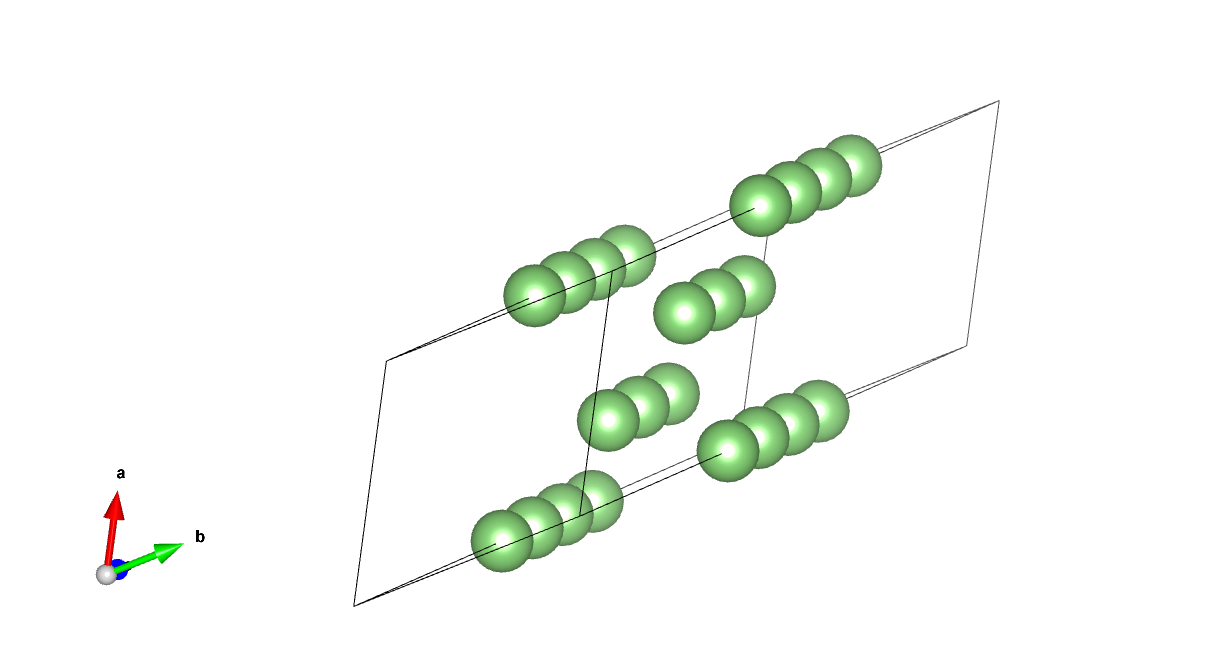
\includegraphics[width=0.45\textwidth]{Li111_pre_mismatch.png}
\hfill
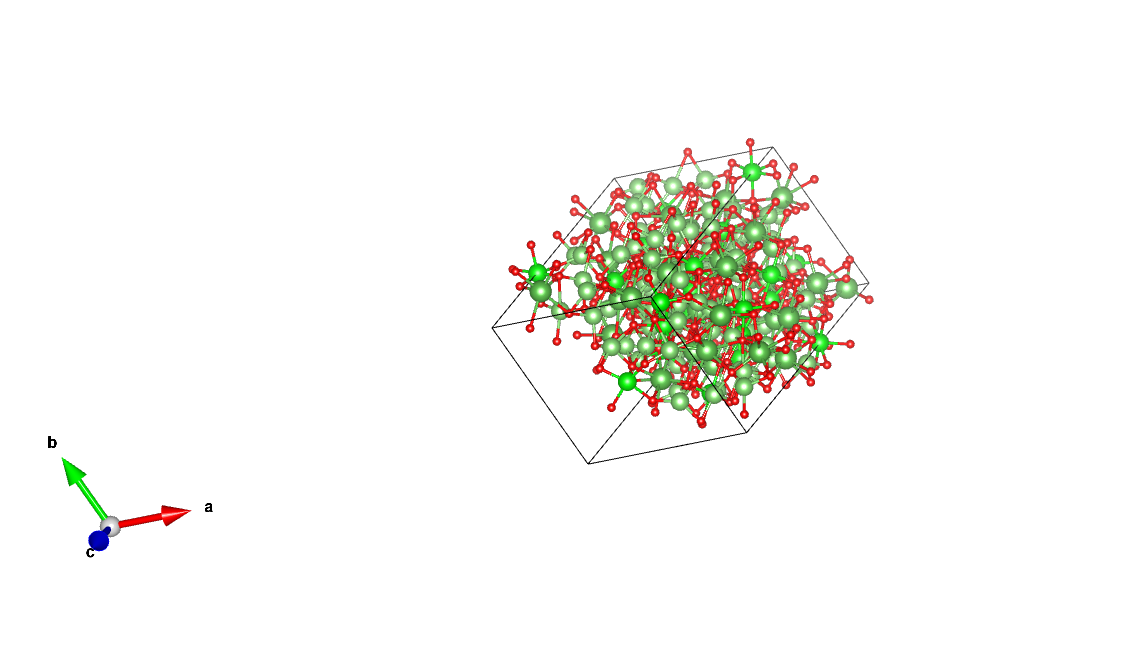
\includegraphics[width=0.45\textwidth]{LLZO_mismatch_example.png}

\vspace{0.5cm}

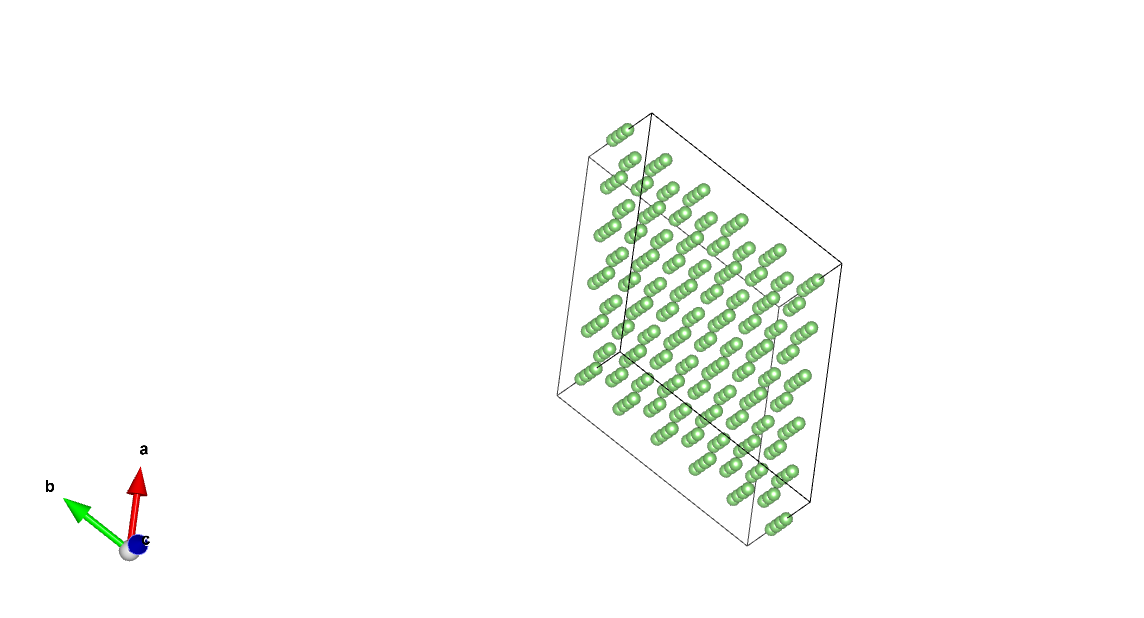
\includegraphics[width=0.45\textwidth]{Li111_after_mismatchScript.png}
\hfill
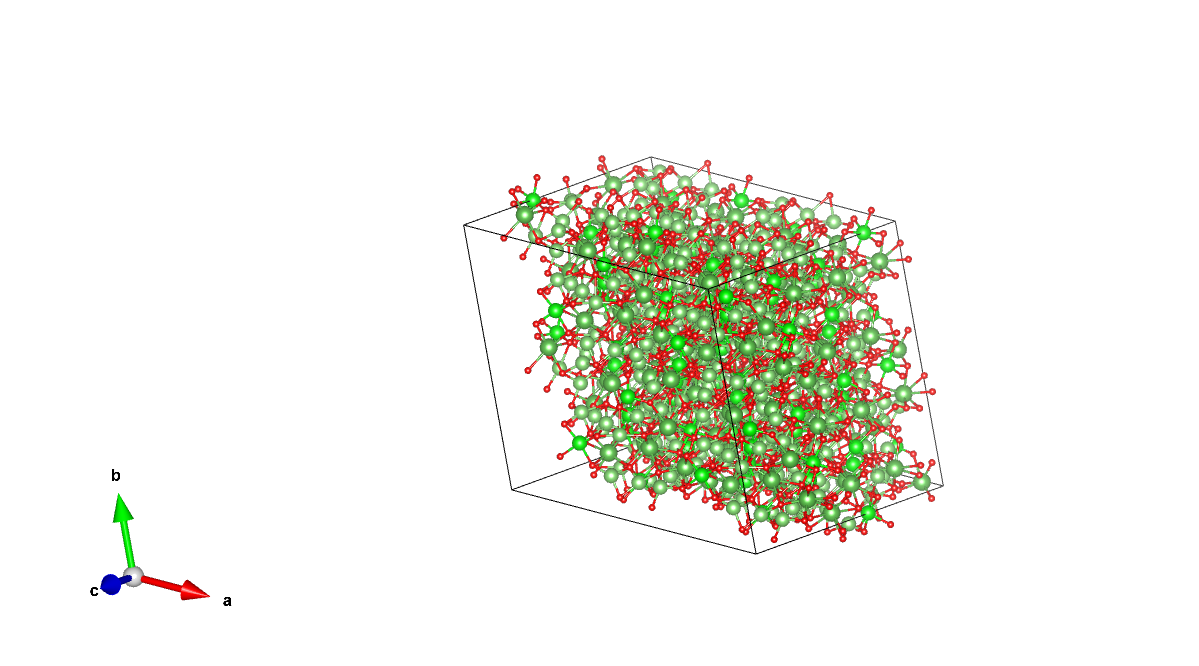
\includegraphics[width=0.45\textwidth]{LLZO_110_aftermatch.png}

\caption{
Example of the lattice matching procedure for a Li(111) and LLZO(110) interface.
Top row: initial slab geometries showing significant in-plane lattice mismatch.
Bottom row: supercell expansion and anisotropic scaling result in matched in-plane
lattice parameters, enabling coherent interface construction.
}
\label{fig:lattice_matching_example}
\end{figure}

For the representative Li(111)--LLZO(110) interface shown in Fig.~\ref{fig:lattice_matching_example},
the initial lithium slab possesses in-plane lattice parameters of approximately
$a = 4.96$~\AA\ and $b = 4.96$~\AA, whereas the LLZO(110) slab exhibits significantly
larger lattice parameters of $a = 11.29$~\AA\ and $b = 11.29$~\AA.

Following the lattice matching procedure, the LLZO slab was expanded to a
$2 \times 2 \times 1$ supercell, resulting in in-plane lattice parameters of
$a = 22.59$~\AA\ and $b = 22.59$~\AA. The lithium slab was correspondingly
expanded and anisotropically scaled to match these values, ensuring consistent
periodic boundary conditions across the interface.

The out-of-plane lattice parameter ($c$) was preserved during this process,
maintaining the slab geometry and vacuum separation.

\section{Interface Construction and Gap Optimization}

\subsection{Interface Stacking}
\label{sec:interface_stacking}

For each lattice-matched Li--LLZO slab pair, interfaces were constructed by
stacking the lithium slab above the LLZO slab along the out-of-plane ($z$) direction.

The initial relative position was defined using the extremal atomic coordinates
of the two slabs. Specifically, the minimum $z$-coordinate of lithium atoms and
the maximum $z$-coordinate of LLZO atoms were used as reference points to define
the interfacial separation.

The lithium slab was translated rigidly along the $z$-direction to achieve a
target interfacial gap, after which the two slabs were combined into a single
periodic structure. The in-plane lattice parameters were kept fixed, consistent
with the lattice matching procedure described previously.

To avoid interactions between periodic images along the surface normal, a vacuum
region of approximately 20~\AA\ (10 both sides) was introduced after stacking, and the structure
was centered along the $z$-direction.

\subsection{Gap Sampling and Energy Evaluation}

To determine physically meaningful interface separations for the initial 
finetuning dataset, a systematic gap scan was performed for each Li--LLZO interface configuration. The interfacial distance
was varied over a range of values:

\begin{equation}
d_{\mathrm{gap}} \in \{1.0, 1.5, 2.0, 2.5, 3.0, 3.5, 4.0\}~\text{\AA}
\end{equation}

For each gap value, the total energy of the stacked structure was evaluated using
a machine learning interatomic potential based on the MACE framework. A pretrained
universal model (MACE-OMAT) was employed for all calculations.

In addition to total energy, the minimum interatomic distance across the interface
was computed to identify potential unphysical atomic overlaps.

\subsection{Selection of Optimal Interface Separation}
\label{sec:gap_opt}

For each Li--LLZO interface, the optimal interfacial gap was selected as the one
corresponding to the lowest total energy, subject to physically reasonable atomic
separations.

The selected configurations typically exhibited minimum interatomic distances of
approximately $1.8$~\AA, indicating the absence of significant atomic overlap while
maintaining close interfacial contact.

This procedure ensures that all interfaces used in subsequent simulations are
initialized from energetically favorable and physically consistent configurations.

\noindent
An example of a constructed interface following this procedure is shown in
Fig.~\ref{fig:stacked_interface_example}, illustrating the relative positioning
of lithium and LLZO slabs after lattice matching and gap optimization.

\begin{figure}[htbp]
\centering
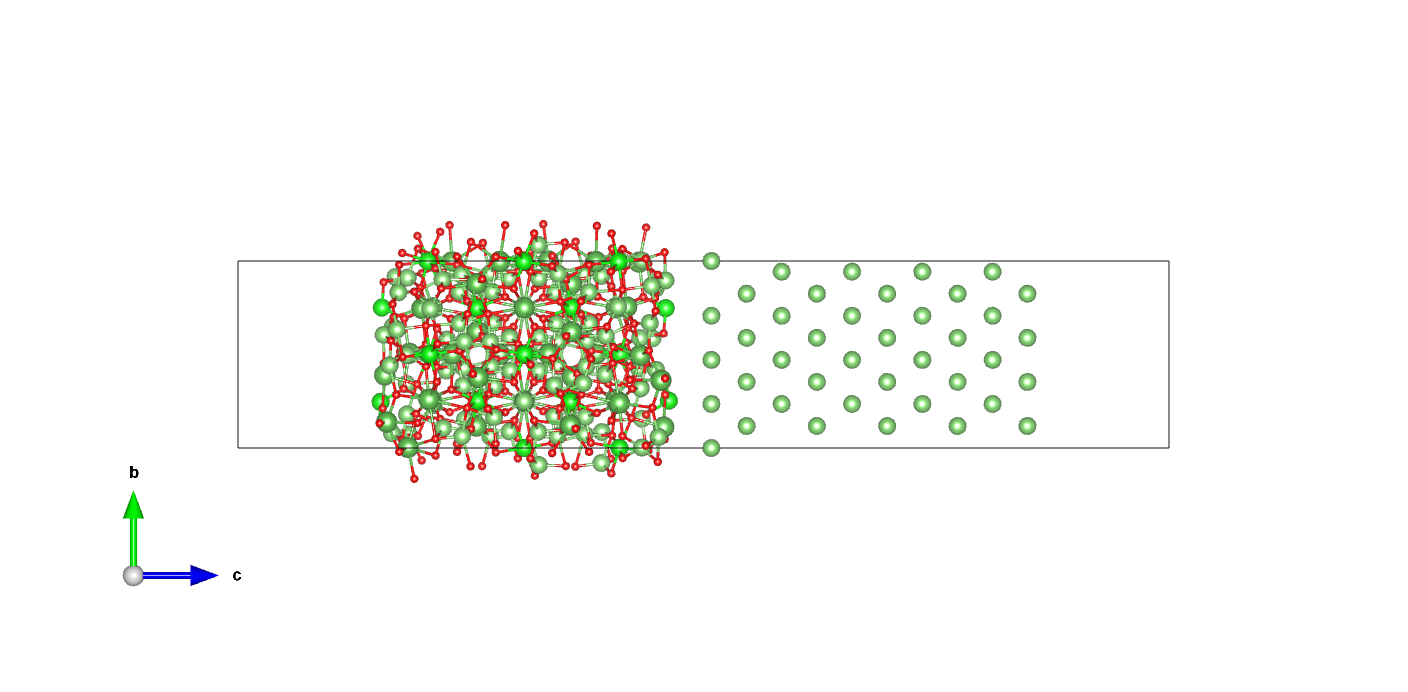
\includegraphics[width=0.8\textwidth]{Li100_LLZO_110_Zr_structure.png}
\caption{
Example of a constructed Li--LLZO interface after lattice matching and gap optimization.
The lithium (Li) slab is stacked on the LLZO(110) Zr-terminated surface. The optimal
interfacial separation was determined to be 3.0~\AA\ based on energy minimization.
The structure shown corresponds to the unrelaxed interface configuration used as
the starting point for subsequent simulations.
}
\label{fig:stacked_interface_example}
\end{figure}

\section{Structural Relaxation}

\subsection{Relaxation Protocol}

All Li--LLZO interface structures obtained after gap optimization were subjected
to structural relaxation to remove residual forces and obtain energetically
stable configurations.

Relaxations were performed using the Atomic Simulation Environment (ASE) with
the universal MACE model, MACE-OMAT.

The FIRE (Fast Inertial Relaxation Engine) algorithm was used for geometry
optimization. Atomic positions were iteratively updated until the maximum force
on any atom satisfied the convergence criterion:

\begin{equation}
F_{\max} < 0.05 \ \text{eV/\AA}
\end{equation}

\subsection{Relaxation Settings and Outputs}

All atoms in the system were allowed to relax without positional constraints.
The lattice parameters were kept fixed during relaxation, preserving the
in-plane lattice matching established during interface construction.

The relaxation procedure was performed for all interface configurations
corresponding to the optimal gap selection described in the previous section.
For each structure, the final relaxed configuration, along with intermediate
trajectories and log files, was recorded for further analysis.

The relaxed interface geometries obtained from this procedure serve as the
starting point for subsequent analysis and experiments.

\section{Molecular Dynamics Simulations}

\subsection{Simulation Objective}

Molecular dynamics (MD) simulations were performed on the relaxed Li--LLZO
interfaces to generate structurally diverse configurations representative of
finite-temperature behavior. This enables sampling of physically relevant
atomic environments near the interface beyond static relaxed geometries.

\subsection{Simulation Setup}
\label{sec:md_sims}

All simulations were carried out using ASE with a universal MACE-OMAT model.
The systems were evolved in the NVT ensemble using a Langevin thermostat.

The integration time step was set to 1~fs, and each simulation was run for
5000 steps at two temperatures, 550~K and 1100~K for each structure obtained from the gap-optimized relaxation procedure described in
Section~\ref{sec:gap_opt}.

\subsection{Active Region and Constraints}

To confine sampling to the interfacially active region and prevent atoms from
diffusing to the cell boundary along the $z$-direction, a geometrically defined active region
was introduced based on atomic positions along the $z$-direction.

The LLZO slab was identified from La, Zr, and O atoms, while lithium metal
was identified as Li atoms located above the LLZO region. For each slab, an
active region was defined near the interface, consisting of approximately
85\% of the slab thickness or a minimum depth of 6~\AA.

Atoms outside this region, primarily in the deeper LLZO layers, were fixed
during MD. This ensures structural stability of the far-bulk region while allowing
physically meaningful atomic motion near the interface.

\subsection{Trajectory Sampling}

Atomic configurations were recorded throughout the MD simulations at regular
intervals (every 25 steps) to capture the evolution of interfacial structures
under finite-temperature conditions.

This sampling strategy generates a diverse set of thermally perturbed atomic
configurations, which are subsequently used for downstream
analysis, including latent space extraction using the universal MACE-OMAT model.

\section{Latent Space Extraction}
\label{sec:latent_extraction}

Following MD trajectory generation, latent embeddings were extracted for all
sampled configurations using the MACE-OMAT universal model. A forward pass
was performed for each structure with force computation enabled, as required
for autograd-based force evaluation. For each atom $i$, the rotationally
invariant ($l = 0$) scalar components of the final message-passing layer were
recorded as a per-atom embedding vector $\mathbf{z}_i \in \mathbb{R}^{256}$.

A structure-level embedding was obtained by mean-pooling over all atoms in
the structure:

\begin{equation}
    \mathbf{Z}_S = \frac{1}{N_S} \sum_{i=1}^{N_S} \mathbf{z}_i
\end{equation}

where $N_S$ is the number of atoms in structure $S$.
The resulting embeddings were stored alongside atomic positions in
\texttt{extxyz} format for downstream use.

\section{Active Learning Structure Selection via Farthest Point Sampling}
\label{sec:fps_method}

Structures for DFT labeling were selected from the MD pool using Farthest
Point Sampling (FPS) in the MACE latent embedding space. The existing
DFT-labeled training set (seed) was included in the initial selected set
$\mathcal{S}_0$ to ensure that newly selected structures complement the
existing training data (For Iteration~0, where no DFT-labeled seed structures were yet available, the
FPS was initialised as the lowest-energy structure evaluated by MACE-OMAT universal model rather than from the
training set centroid since no prior assumptions on distribution was assumed).

At each step, the distance of each pool candidate to its nearest
already-selected structure was computed:

\begin{equation}
    \delta_k = \min_{\mathbf{Z}_s \in \mathcal{S}}\,
    \|\mathbf{Z}_k - \mathbf{Z}_s\|_2
\end{equation}

The candidate with the largest $\delta_k$ was selected and added to
$\mathcal{S}$. This was repeated until the target number of structures was
reached. Selected structures were subsequently submitted for DFT single-point
energy and force calculations and incorporated into the training set for the
next model iteration. As described in Section~\ref{sec:latent_extraction}, structures that are distant in the 
MACE latent space represent chemically distinct local environments --- a strictly 
stronger signal for active learning than geometric diversity alone, since the 
learned representation already encodes many-body chemical interactions.

\section{Coverage Statistics}
\label{sec:coverage_stats_methods}

To quantitatively assess the extent to which the selected structures cover
the pool's distribution in latent space, a set of coverage metrics was
computed both before and after FPS selection.

\paragraph{Per-point coverage distance --}
For each structure $k$ in the pool $\mathcal{P}$, the distance to its
nearest selected neighbour in $\mathcal{S}$ was defined as:

\begin{equation}
    \delta_k = \min_{\mathbf{Z}_s \in \mathcal{S}}\,
    \|\mathbf{Z}_k - \mathbf{Z}_s\|_2
\end{equation}

The distribution of $\{\delta_k\}_{k \in \mathcal{P}}$ characterises how
uniformly the selected set covers the pool: a narrow distribution concentrated
near zero indicates thorough coverage, while a heavy tail indicates regions of
latent space that remain underrepresented.

\paragraph{Coverage radius --}
The coverage radius of a selected set $\mathcal{S}$ with respect to pool
$\mathcal{P}$ is defined as:

\begin{equation}
    \rho(\mathcal{S}, \mathcal{P}) = \max_{k \in \mathcal{P}}\, \delta_k
\end{equation}

This is the worst-case distance from any pool point to its nearest selected
neighbour. FPS minimises $\rho$ greedily: each step reduces the maximum
uncovered distance as much as possible. A smaller $\rho$ implies better
worst-case coverage.

\paragraph{Percentile coverage --}
To obtain a threshold-independent summary statistic, the fraction of pool
structures covered within a distance of $d$ by the selected set was computed:

\begin{equation}
    C(d) = \frac{1}{|\mathcal{P}|} \sum_{k \in \mathcal{P}}
    \mathbf{1}\!\left[\delta_k \leq d\right]
\end{equation}

$C(d)$ is a monotonically increasing function ranging from $0$ to $1$.
The area under $C(d)$ provides a scalar summary of overall coverage quality,
analogous to the area under an ROC curve.

\paragraph{Seed vs.\ pool comparison --}
Coverage was evaluated separately for the following groups within the pool:
\begin{itemize}
    \item MD frames from each interface configuration and temperature
    \item External structures from prior DFT datasets (where applicable)
\end{itemize}

This allows assessment of whether the FPS selection achieves uniform coverage
across different chemical environments and thermal conditions, or whether
certain configurations are systematically underrepresented in the training
data.

Coverage distributions were computed before FPS (baseline: seed $\mathcal{S}_0$
covering pool $\mathcal{P}$) and after FPS (updated $\mathcal{S}$ covering
remaining pool), providing a direct quantification of the information gain
achieved by each iteration of structure selection.

\section{Iterative Active Learning Framework}

\subsection{Overview}

The active learning procedure employed in this work follows an iterative
loop in which new interface configurations are progressively introduced,
latent space coverage is evaluated, diverse structures are selected for
DFT labeling, and the MACE model is finetuned on the augmented dataset.
This process is repeated across multiple iterations, with the model's
coverage of the relevant chemical space improving at each step.

The general structure of the loop is summarised as follows. Let $\mathcal{T}^{(n)}$
denote the DFT-labeled training set at iteration $n$, and let
$\theta^{(n)}$ denote the model parameters after finetuning on
$\mathcal{T}^{(n)}$. The procedure at each iteration is:

\begin{enumerate}
    \item \textbf{MD sampling.} Run NVT molecular dynamics on the current set of
    interface configurations using the model $\theta^{(n)}$. Record trajectory
    frames at regular intervals to form a pool $\mathcal{P}^{(n)}$.

    \item \textbf{Configuration expansion.} Introduce one or more new interface
    configurations not previously included in the MD pool. Evaluate their
    embeddings using $\theta^{(n)}$ and embed them in the current latent space.
    Compute coverage distances $\delta_k$ relative to $\mathcal{T}^{(n)}$ to
    determine whether these configurations lie in underrepresented regions.

    \item \textbf{Latent embedding.} Extract mean-pooled MACE embeddings
    $\mathbf{Z}_S$ for all structures in the expanded pool
    $\mathcal{P}^{(n)} \cup \mathcal{P}^{(n)}_{\mathrm{new}}$.

    \item \textbf{Structure selection.} Apply FPS in embedding space
    (seeded with $\mathcal{T}^{(n)}$) to select $k^{(n)}$ structures
    from the pool for DFT labeling.

    \item \textbf{DFT labeling.} Compute single-point energies and forces
    for the selected structures using DFT. Add the labeled structures to
    the training set: $\mathcal{T}^{(n+1)} = \mathcal{T}^{(n)} \cup \mathcal{L}^{(n)}$.

    \item \textbf{Finetuning.} Finetune the MACE model on $\mathcal{T}^{(n+1)}$
    to obtain $\theta^{(n+1)}$.

    \item \textbf{Repeat.} Increment $n$ and return to step 1.
\end{enumerate}

\subsection{Iteration 0: Initial Finetuning}

Prior to the first full active learning iteration, an initial finetuning
step was performed using 20 structures selected from the initial MD pool.
Because no DFT-labeled interface training set was available at Iteration~0,
FPS was initialized from the lowest-energy structure evaluated using the
MACE-OMAT universal model. The remaining structures were then selected
iteratively by farthest point sampling in the MACE latent space, so that the
final set of 20 configurations spanned diverse and underrepresented regions
of the initial pool. DFT single-point calculations were performed on these
structures, and the model was finetuned to produce $\theta^{(1)}$.
\subsection{Super-FPS: Two-Stage Structure Selection}

In subsequent iterations, a two-stage selection procedure was employed to
select maximally informative structures from large candidate pools while
minimizing the number of expensive DFT calculations. This procedure, referred
to here as Super-FPS, is designed to retain global diversity in the pool while
ensuring that the final selected structures are complementary to the structures
already present in the training set.

In the first stage, a coarse FPS pass was applied to the full pool
$\mathcal{P}^{(n)}$ using the previous iteration training set
$\mathcal{T}^{(n)}$ as the seed set. This produced a diverse intermediate
candidate set of $M$ structures, denoted $\mathcal{Q}^{(n)}$:

\begin{equation}
    \mathcal{Q}^{(n)} =
    \mathrm{FPS}\!\left(\mathcal{P}^{(n)},\mathcal{T}^{(n)},M\right).
\end{equation}

In the second stage, a fine FPS pass was applied only to the coarse candidate
set $\mathcal{Q}^{(n)}$, again using the current training set
$\mathcal{T}^{(n)}$ as the seed set. This selected the final
$k^{(n)}$ structures for DFT labeling:

\begin{equation}
    \mathcal{L}^{(n)} =
    \mathrm{FPS}\!\left(\mathcal{Q}^{(n)},\mathcal{T}^{(n)},k^{(n)}\right).
\end{equation}

Here, $\mathrm{FPS}(\mathcal{A},\mathcal{S}_0,k)$ denotes $k$-step greedy
farthest point sampling on the candidate set $\mathcal{A}$, initialized with
the seed set $\mathcal{S}_0$. In this work, $M=20$ was used for the coarse
pass, and $k^{(n)}=6$ structures were selected for DFT labeling in Iteration~1.

The first stage reduces the full MD and external-structure pool to a compact
set of diverse candidates, while the second stage selects final structures
that are well separated from the existing training set in the MACE latent space. Coverage statistics were then computed after selection to
quantify how much of the pool was represented by the selected structures.
\subsection{Progressive Interface Expansion}

At each iteration, one or more new Li--LLZO interface configurations
(e.g., a new surface termination or crystallographic orientation) were
introduced into the simulation pool. Before incorporating MD frames
from these configurations, their latent embeddings under the current
model $\theta^{(n)}$ were computed and their coverage distances
$\delta_k$ relative to $\mathcal{T}^{(n)}$ were examined.

If the new configurations exhibited large coverage distances --- indicating
that their local chemical environments are poorly represented in the
current training set --- MD frames from those configurations (or related
configurations with similar surface chemistry) were included in the
expanded pool $\mathcal{P}^{(n)}_{\mathrm{new}}$ and were eligible for
selection in the subsequent FPS pass.

This progressive expansion strategy ensures that the active learning loop
systematically improves model accuracy across the full range of interface
geometries considered in this study, not just those present in the
initial configuration pool.

\subsection{Finetuning Protocol --- Low-Rank Adaptation (LoRA)}

At each iteration, the MACE model was finetuned starting from the
parameters $\theta^{(n)}$ using the updated training set
$\mathcal{T}^{(n+1)}$. Finetuning was performed using the standard
MACE training pipeline with low-rank adaptation (LoRA) to preserve the general chemical knowledge 
of the bulk phases already encoded in the pretrained universal model, which 
would otherwise be overwritten by standard full-parameter gradient descent 
on the small interface dataset, hence preventing catastrophic forgetting.
The LoRA rank was chosen to be 5 and LoRA $\alpha$ was chosen to be 1.0 based on hyperparameter tuning, avoiding both underfit and overfit.

The finetuned model $\theta^{(n+1)}$ was subsequently used for all
downstream MD simulations, latent space extraction, and coverage
evaluation in iteration $n+1$.

\subsection{Low-Rank Adaptation (LoRA) Fine-Tuning of MACE}

To adapt the pretrained MACE foundation model (MACE-OMAT) to the Li--LLZO interface dataset, we employ Low-Rank Adaptation (LoRA), a parameter-efficient fine-tuning strategy~\cite{LoRA2021}. MACE directly exposes LoRA fine-tuning within its default training framework through dedicated flags, enabling seamless integration into standard training workflows.\footnote{\href{https://mace-docs.readthedocs.io/en/latest/guide/lora_finetuning.html}{mace-docs: LoRA finetuning}}Instead of updating all model parameters during training, LoRA constrains the weight updates to a low-rank subspace, thereby reducing the number of trainable parameters and mitigating overfitting on small datasets. In this approach, the pretrained weights are frozen, and only a small set of low-rank adapter matrices are trained, significantly improving computational efficiency while preserving the generalization capability of the foundation model.

\subsubsection{LoRA Formulation}

Let $W \in \mathbb{R}^{d \times d}$ denote a weight matrix in the pretrained model. In standard fine-tuning, the updated weights are given by:
\begin{equation}
W' = W + \Delta W,
\end{equation}
where $\Delta W$ is a full-rank update.

In LoRA, the update is factorized as:
\begin{equation}
\Delta W = BA,
\end{equation}
where
\begin{equation}
A \in \mathbb{R}^{r \times d}, \quad B \in \mathbb{R}^{d \times r},
\end{equation}
and $r \ll d$ is the rank of the adaptation. The forward pass is then modified as:
\begin{equation}
y = \left(W + \frac{\alpha}{r} BA \right) x,
\end{equation}
where $\alpha$ is a scaling factor controlling the magnitude of the update.

In this work, we use a LoRA rank of $r = 5$ and scaling factor $\alpha = 1.0$.

\subsubsection{Equivariant LoRA in MACE}

MACE employs $O(3)$-equivariant neural networks to ensure rotational symmetry of atomic interactions. To preserve equivariance, LoRA adapters are introduced within equivariant linear layers (e.g., \texttt{o3.Linear}) and dense layers, ensuring that the low-rank updates respect the underlying symmetry constraints.

The modified equivariant layer takes the form:
\begin{equation}
h_{\text{out}} =
W h_{\text{in}} +
\frac{\alpha}{r} B (A h_{\text{in}}),
\end{equation}
where $W$ denotes frozen pretrained weights, and $A, B$ are trainable equivariant projections constructed using compatible irreducible representations.

\subsubsection{Parameter Freezing and Efficiency}

During training, all pretrained parameters $\theta_{\text{base}}$ are frozen:
\begin{equation}
\nabla_{\theta_{\text{base}}} L = 0,
\end{equation}
and only the LoRA parameters $(A, B)$ are optimized:
\begin{equation}
\nabla_{A,B} L \neq 0.
\end{equation}

This reduces the number of trainable parameters from $\mathcal{O}(d^2)$ per layer to $\mathcal{O}(2rd)$, which in practice corresponds to less than 1\% of the full model parameters.

\subsubsection{Initialization}

To ensure that the model initially reproduces the pretrained behavior, the LoRA parameters are initialized as:
\begin{equation}
A \sim \mathcal{N}(0, 10^{-3}), \quad B = 0,
\end{equation}
such that:
\begin{equation}
\Delta W = BA = 0, \quad W' = W.
\end{equation}

The model therefore starts from the pretrained state and gradually learns task-specific corrections during training.

\subsubsection{Training Objective}

The model is trained on a dataset
\begin{equation}
D = \{(R_i, E_i, F_i)\}_{i=1}^{N},
\end{equation}
where $R_i$ are atomic positions, $E_i$ are total energies, and $F_i$ are atomic forces.

The loss function is defined as:
\begin{equation}
L =
w_E \sum_i (E_i - \hat{E}_i)^2 +
w_F \sum_i \|F_i - \hat{F}_i\|^2,
\end{equation}
with weights $w_E = 1$ and $w_F = 10$.

\subsubsection{Model Construction}

Starting from the pretrained MACE-OMAT model, LoRA fine-tuning is performed on a small seed dataset selected via farthest point sampling. The resulting adapted model is given by:
\begin{equation}
\theta_{\text{adapted}} =
\theta_{\text{base}} +
\frac{\alpha}{r} BA.
\end{equation}

For deployment, the low-rank updates are merged into the base weights:
\begin{equation}
W_{\text{final}} = W + BA,
\end{equation}
yielding a standard MACE model with no additional computational overhead at inference time.

\subsection{Generalisation of the Framework}

The active learning loop described above is not specific to the Li--LLZO
system and can be generalised to any interface or heterogeneous material
system for which:
\begin{itemize}
    \item A pretrained MACE (or compatible equivariant GNN) model
    is available for initial MD and embedding extraction,
    \item DFT single-point calculations can be performed to label
    selected structures, and
    \item A sufficiently diverse set of interface configurations can
    be constructed to define the relevant chemical space.
\end{itemize}

The two key design choices --- latent-space FPS for selection and
progressive interface expansion for coverage --- are broadly applicable
and can be combined with any compatible active learning infrastructure
or labeling oracle.

%% CHANGED: added label so broken \ref{...} can be resolved
\section{DFT Labeling of Selected Structures}
\label{sec:dft_labeling}

\subsection{Overview}

Structures selected via the active learning pipeline were labeled using Density Functional Theory (DFT) calculations to obtain ground-state energies and atomic forces. These labels serve as the reference data for subsequent model finetuning.

All DFT calculations were performed using the real-space finite-element code \textsc{DFT-FE}, which is well-suited for large, non-periodic slab systems and enables efficient GPU-accelerated simulations given that the interface supercells contain 500--1500 atoms.

\subsection{Electronic Structure Setup}

The electronic structure calculations were carried out within the framework of Kohn--Sham DFT using the generalized gradient approximation (GGA) in the Perdew--Burke--Ernzerhof (PBE) form for the exchange--correlation functional.

Norm-conserving pseudopotentials were employed for all atomic species (Li, La, Zr, O). The pseudopotential files were consistently used across all calculations to ensure uniformity of the dataset. The dataset used was SPMS Pseudopotentials \footnote{\url{https://github.com/SPARC-X/SPMS-psps}}, which are soft and transferable pseudopotentials from multi-objective optimization.

Self-consistent field (SCF) calculations were performed with a Fermi--Dirac smearing corresponding to an electronic temperature of 500~K. Convergence was achieved with a tolerance of $5 \times 10^{-5}$ Ha on the electronic energy.

All interface structures were treated as slab geometries with periodic
boundary conditions applied in the in-plane directions ($x$ and $y$),
and non-periodic boundary conditions along the surface normal ($z$).
For all 26 labeled structures used in the dataset, zero Dirichlet
boundary conditions were imposed along the non-periodic direction for
both the wavefunctions and the electrostatic potential.

To verify that the interfacial dipole does not materially affect the
DFT labels, 4 representative structures were additionally recomputed
using an alternative electrostatic boundary condition: zero Dirichlet
for the wavefunctions and Neumann (zero-flux) for the electrostatic
potential. Among these checks, two representative interfaces ---
Li(111)/LLZO(011)-La and Li(111)/LLZO(110)-Li --- were examined in
detail. The total energy difference was $\mathcal{O}(10^{-6})$~Ha and
the maximum force difference was $\sim 5\times10^{-5}$~Ha/Bohr
($\sim$2.6~meV/\AA), well below the MLIP training noise floor of
$\sim$50~meV/\AA. This confirms that the choice of electrostatic
boundary condition has negligible effect on the training labels for the
interface geometries studied here.

This treatment stands in contrast to conventional plane-wave DFT codes,
which enforce full three-dimensional periodicity. For an asymmetric
Li$|$LLZO slab, plane-wave codes generally require either a symmetric
Li$|$LLZO$|$Li sandwich geometry or an asymmetric slab with a large
vacuum region together with a post-hoc dipole correction to suppress
spurious periodic-image interactions. Prior first-principles studies of
the Li--LLZO interface, including Iwasaki et
al.~\cite{Iwasaki2022DFT_Li_LLZO_PSSB} and Burov et
al.~\cite{Burov2024LiLLZOChargeTransfer}, were conducted with
plane-wave codes and therefore face these constraints. DFT-FE's native
mixed boundary-condition framework avoids these workarounds and enables
direct asymmetric single-interface slab calculations at the 450--1500
atom scale used for MLIP training labels in this work.
\subsection{Finite Element Discretization}

The Kohn--Sham equations were discretized using a high-order finite-element basis with polynomial order 7. The computational mesh was generated automatically with refinement in the vicinity of atomic cores, using a mesh size parameter of 1.2~\AA\ and an atom-centered refinement radius of 8.0~\AA.

This high-order discretization ensures accurate resolution of both the electronic density and the resulting forces, particularly in heterogeneous interface environments.

\subsection{Force Evaluation}

For each selected configuration, single-point DFT calculations were performed to compute total energies and atomic forces. No structural relaxation was carried out at this stage, as the objective is to obtain accurate force labels for the active learning process.

\subsection{Computational Details}

All DFT calculations were performed on the OLCF \textit{Frontier} supercomputing system using GPU acceleration. Calculations were distributed across 64 nodes (each node with 1 x Optimized 3rd Gen AMD EPYC CPU + 4 x MI250X GPUs) with one MPI task per GPU, enabling efficient parallel execution.

The DFT-FE solver was operated in ground-state (GS) mode with Anderson mixing for SCF convergence. Memory optimization and GPU acceleration were enabled to ensure efficient handling of large interface systems, for the interface supercells studied here, which contain 450--1500 atoms.

All production labels in the dataset were generated using identical computational settings; the Neumann-boundary calculations were performed only as auxiliary validation checks.

Model training, inference, and MD simulations were carried out on the KIAC 
Mahamathi cluster (NVIDIA H200 GPUs) and the ALCF Polaris supercomputer 
(NVIDIA A100 GPUs). DFT single-point calculations were performed on the 
OLCF Frontier supercomputer, as described in \secref{sec:dft_labeling}.


\section{Bulk cohesive-energy calculation}

In addition to energy and force errors on interface configurations, the trained models were validated against bulk cohesive energies of bcc Li and bulk LLZO. This serves as an important consistency check because subsequent interface energetics, including work of adhesion and interface formation energies, depend on reliable bulk reference states.

For a structure containing \(N\) atoms, the cohesive energy per atom was computed as
\begin{equation}
E_{\mathrm{coh}} = \frac{E_{\mathrm{bulk}} - \sum_i n_i E_i^{\mathrm{atom}}}{N},
\end{equation}
where \(E_{\mathrm{bulk}}\) is the total energy of the periodic bulk structure, \(E_i^{\mathrm{atom}}\) is the isolated-atom reference energy of element \(i\), and \(n_i\) is the number of atoms of species \(i\) in the structure. With this convention, bound solids have negative cohesive energies.

For Li and LLZO, DFT reference cohesive energies were computed from Quantum ESPRESSO calculations on the corresponding periodic bulk cells. Quantum ESPRESSO was used since it is a much faster alternative on smaller systems than DFT-FE, and the two codes have been shown to yield consistent total energies and forces
for norm-conserving pseudopotential calculations~\cite{Das2022}. The Li bulk reference consisted of a two-atom bcc conventional cell with a \(4\times4\times4\) Monkhorst--Pack grid, while LLZO was evaluated using the 192-atom conventional bulk cell with a \(3\times3\times3\) grid. In both cases, PBE exchange--correlation, SPMS norm-conserving pseudopotentials, and an 80 Ry plane-wave cutoff were used. The same cohesive-energy definition was then applied to the ML models. For the task-specific finetuned models (Iteration 0 and Iteration 1), isolated-atom energies were obtained directly from the corresponding model. For the universal MACE-OMAT model, externally aligned single-atom reference energies were used instead of the model-native isolated-atom energies, since the pretrained model is not directly aligned for absolute atomic reference energies.

The Li bulk cohesive-energy reference was computed using a two-atom bcc Li cell with lattice parameter 3.4393~\AA\ and a \(3\times3\times3\) \(k\)-point mesh. The LLZO bulk cell corresponds to the ordered tetragonal polymorph 
($I4_1/acd$) of Li$_7$La$_3$Zr$_2$O$_{12}$~\cite{Murugan2007}, 
which serves as the bulk reference state for all interface energetics 
in this work. The LLZO cohesive-energy reference was computed using the 192-atom conventional bulk cell with lattice parameters \(a=b=13.23607\)~\AA\ and \(c=12.701706\)~\AA, sampled using a \(3\times3\times3\) mesh. Both calculations were performed in Quantum ESPRESSO using PBE, SPMS norm-conserving pseudopotentials, Fermi--Dirac smearing, and an 80 Ry plane-wave cutoff. The LLZO input used the corrected bulk structure and \(3\times3\times3\) \(k\)-point sampling, while the Li input also used the \(3\times3\times3\) mesh for the two-atom bcc cell. 

\chapter{Results and Discussion}
\label{ch:results}
\section{Iteration~0 Finetuning}
\label{sec:results_it0}

\subsection{Finetuning Dataset}

The initial dataset for the active learning loop (denoted as Dataset$_0$) was constructed from molecular dynamics (MD) sampling of a diverse set of Li--LLZO interface configurations.

Interface structures were generated by combining lithium slabs with crystallographic orientations (100), (110), and (111), with LLZO surfaces spanning multiple terminations and orientations, including:
\begin{itemize}
    \item (001) and (110) Zr-terminated surfaces,
    \item (010) and (011) La-terminated surfaces,
    \item (021) and (110) Li-terminated surfaces.
\end{itemize}

From this combinatorial space, 18 initial interface configurations were constructed following the lattice matching and gap optimization procedure described in Chapter 3. These structures were subsequently relaxed using the MACE-OMAT universal model. Only structures that achieved a force convergence criterion of $F_{\max} < 0.05$~eV/\AA\ were retained, resulting in a filtered set of 13 relaxed interface configurations.

\paragraph{Gap optimization --}
Gap optimization was performed as described in Section~\ref{sec:gap_opt}. 
The selected interfacial separations ranged between 2.0~\AA\ and 3.0~\AA, 
with minimum interatomic distances consistently around $\sim$1.8~\AA\ across 
all retained configurations.

\paragraph{MD sampling --}
MD simulations were performed as described in Section~\ref{sec:md_sims} on all 
13 converged interface configurations (13 of 18 initial structures passed the 
$F_{\max} < 0.05$~eV/\AA\ convergence criterion). To enhance sampling of 
high-energy configurations, an extended trajectory of 20{,}000 steps at 1100~K 
was additionally performed for a representative Li(100)/LLZO(001) Zr-terminated 
interface. The combined pool comprised $\sim$5{,}300 configurations with system 
sizes ranging from $\sim$450 to $\sim$1{,}500 atoms (mean $\sim$700 atoms).

\subsection{Structural Representation and Active Learning Selection}
\label{sec:fps_selection}

To efficiently select representative configurations from the extensive pool of generated molecular dynamics (MD) trajectories for the next active learning iteration, we leverage the internal representations of the pre-trained MACE model. Rather than relying on simple geometric heuristics, the latent node embeddings from the final message-passing layer of the MACE architecture are pooled to generate a 256-dimensional global embedding vector for each structural snapshot. This embedding encapsulates rich, many-body quantum mechanical descriptors of the local chemical environments.

Latent embeddings were extracted, normalized, and projected as described in 
Sections~\ref{sec:latent_extraction} and~\ref{sec:fps_method}. After filtering 
configurations with positive predicted energies, a viable pool of 5{,}297 
structures remained. Embeddings were projected onto 32 principal components, 
capturing $\geq$99.9\% of total structural variance.

\subsubsection{Farthest Point Sampling and Coverage Statistics}
To maximize the informativeness of the next batch of Density Functional Theory (DFT) calculations and avoid selecting redundant configurations, we employ a Farthest Point Sampling (FPS) algorithm over the PCA-reduced latent space. The FPS algorithm is seeded deterministically with the lowest-energy configuration (a thermodynamically stable $\text{Li}(111)/\text{LLZO}(011)$ La-terminated interface at 550 K) to anchor the dataset. Subsequently, the algorithm iteratively evaluates the remaining pool and selects the structure that maximizes the minimum Euclidean distance to all previously selected states.

A quantitative analysis of the precisely selected $K=20$ configurations reveals that the FPS algorithm successfully sampled a highly diverse and unbiased subset of the configurational phase space, preventing over-representation of any single interface type. The breakdown of the selected structures is as follows:

\begin{itemize}
    \item \textbf{Li Metal Orientations:} The subset is composed of 60\% Li(100) interfaces (12 structures), 30\% Li(110) interfaces (6 structures), and 10\% Li(111) interfaces (2 structures).
    \item \textbf{LLZO Solid Electrolyte Terminations:} The algorithm explored a broad range of ceramic terminations, capturing 6 Zr-terminated LLZO(001) surfaces, 5 La-terminated LLZO(011) surfaces, 5 Li-terminated LLZO(110) surfaces, and 4 La-terminated LLZO(010) surfaces.
    \item \textbf{Thermodynamic Regimes:} The selection exhibits a strong preference for high-temperature regimes, extracting 12 structures from 1100 K trajectories (60\%) and 8 structures from 550 K trajectories (40\%).
\end{itemize}

The preference for 1100 K structures highlights the utility of FPS: at higher temperatures, atoms undergo larger structural distortions and phase-space excursions. These distorted representations inherently lie at the farthest geometric boundaries of the dataset's latent space, which is precisely what the active learning scheme requires to improve out-of-distribution (OOD) generalization.

Figures \ref{fig:fps_pca_2d} and \ref{fig:fps_pca_3d} illustrate the 2D and 3D dimensionality-reduced projections of the structural latent space, respectively. The visuals annotate the FPS-selected configurations with their specific interface orientations and simulation temperatures. By successfully populating the sparse, outermost boundaries of the latent manifold, the selected subsets guarantee a robust, diverse, and maximally informative training batch for the next iteration of the active learning pipeline.

\begin{figure}[htbp]
    \centering
    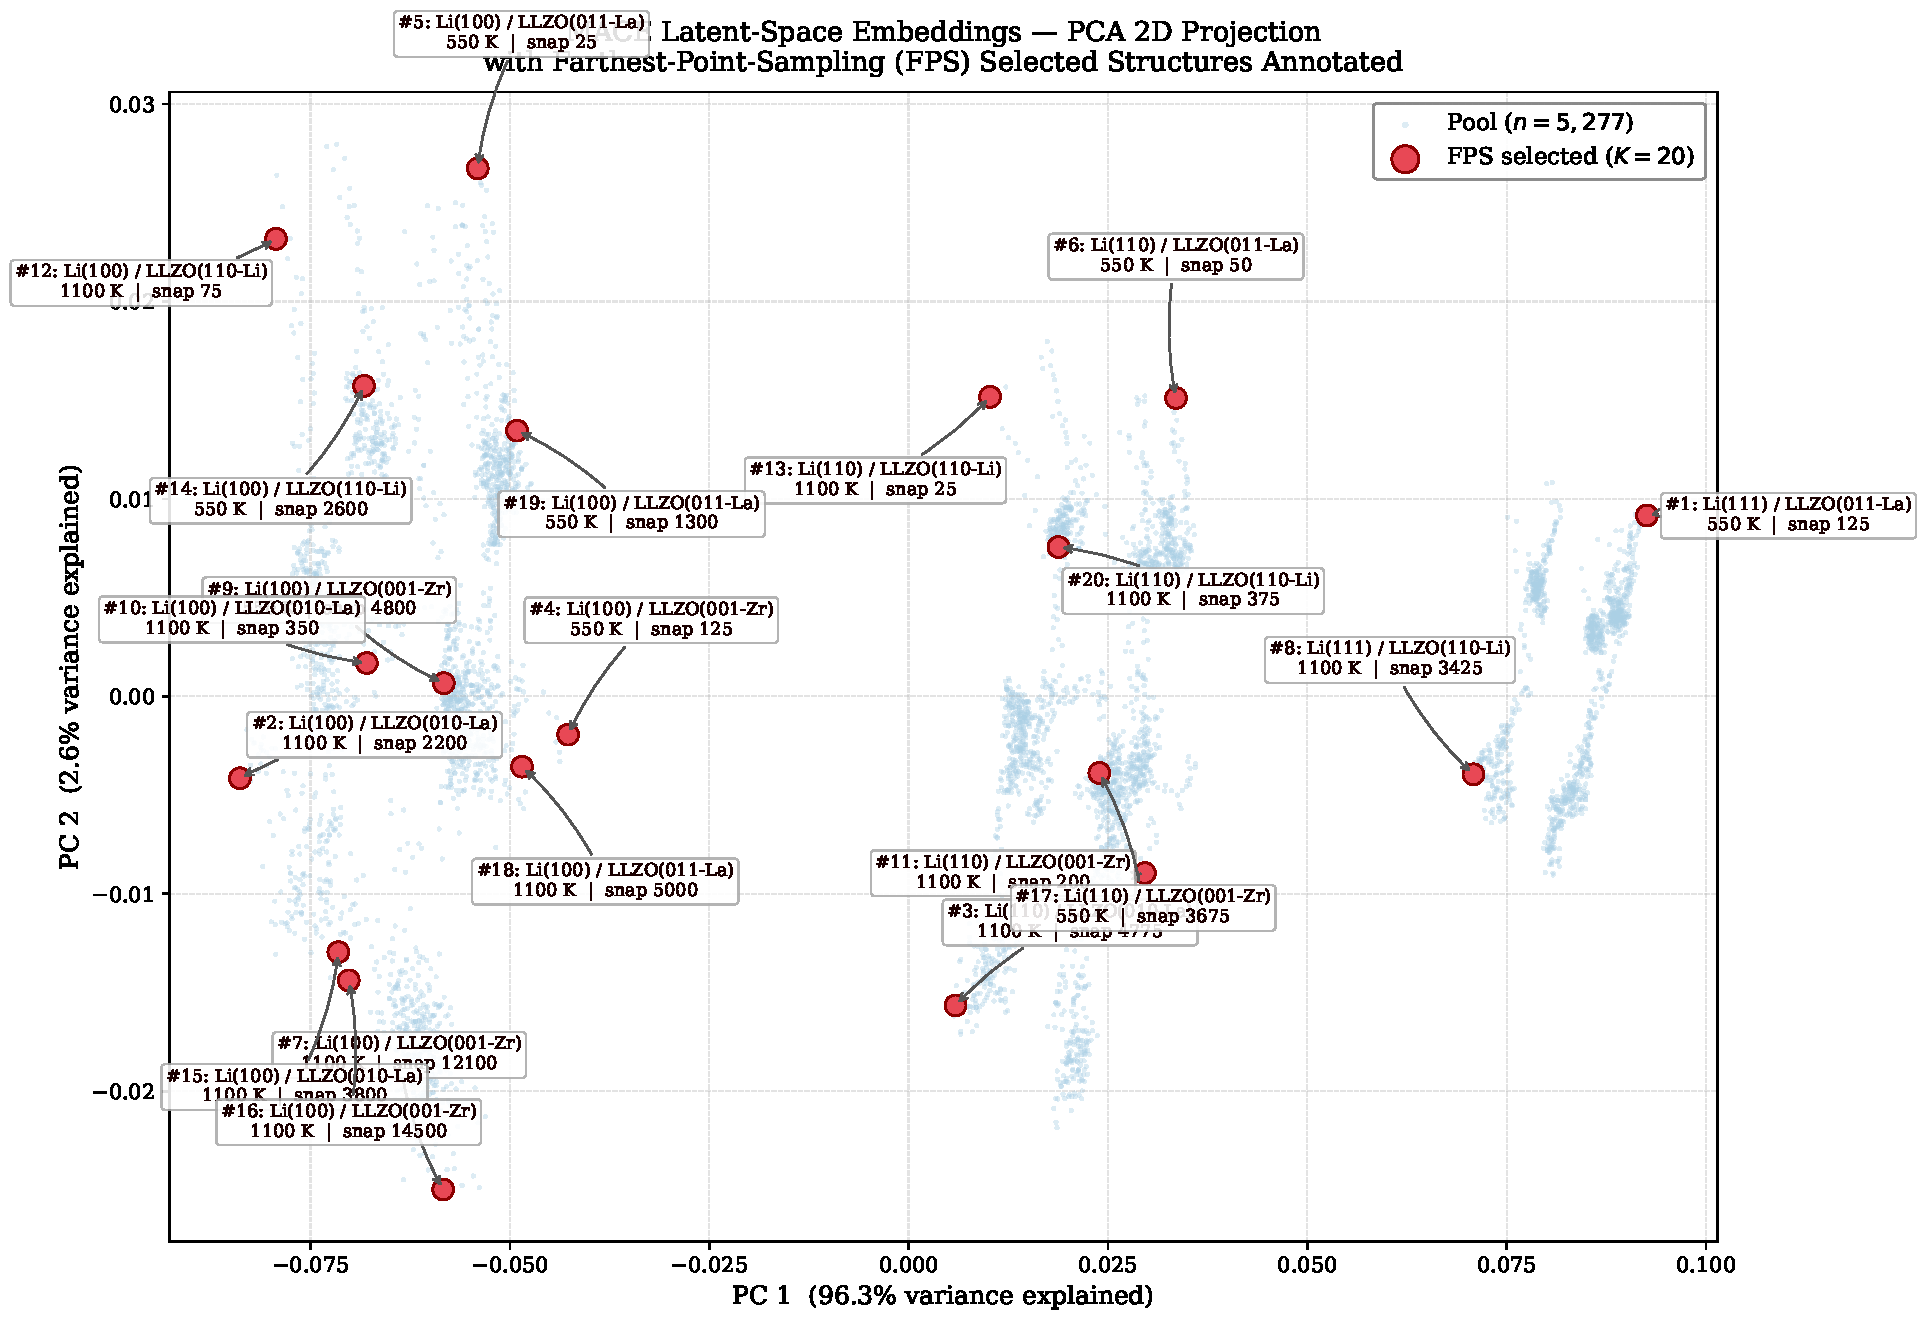
\includegraphics[width=1\textwidth]{fps_embedding_2d.pdf}
    \caption{2D PCA projection (PC1 vs PC2) of the MACE latent-space embeddings for the pool of 5,297 valid Li/LLZO interface structures. The $K=20$ configurations selected via Farthest Point Sampling (FPS) are highlighted in red and explicitly annotated with their respective Li facets, LLZO terminations, and MD simulation temperatures. The FPS algorithm is shown to span the boundaries of the sampled configuration space, selecting structures from the outermost regions of the latent manifold. Note that even though the points lie close on this 2D map, the FPS was done in 32D, where these still lie further apart.}
    \label{fig:fps_pca_2d}
\end{figure}

\begin{figure}[htbp]
    \centering
    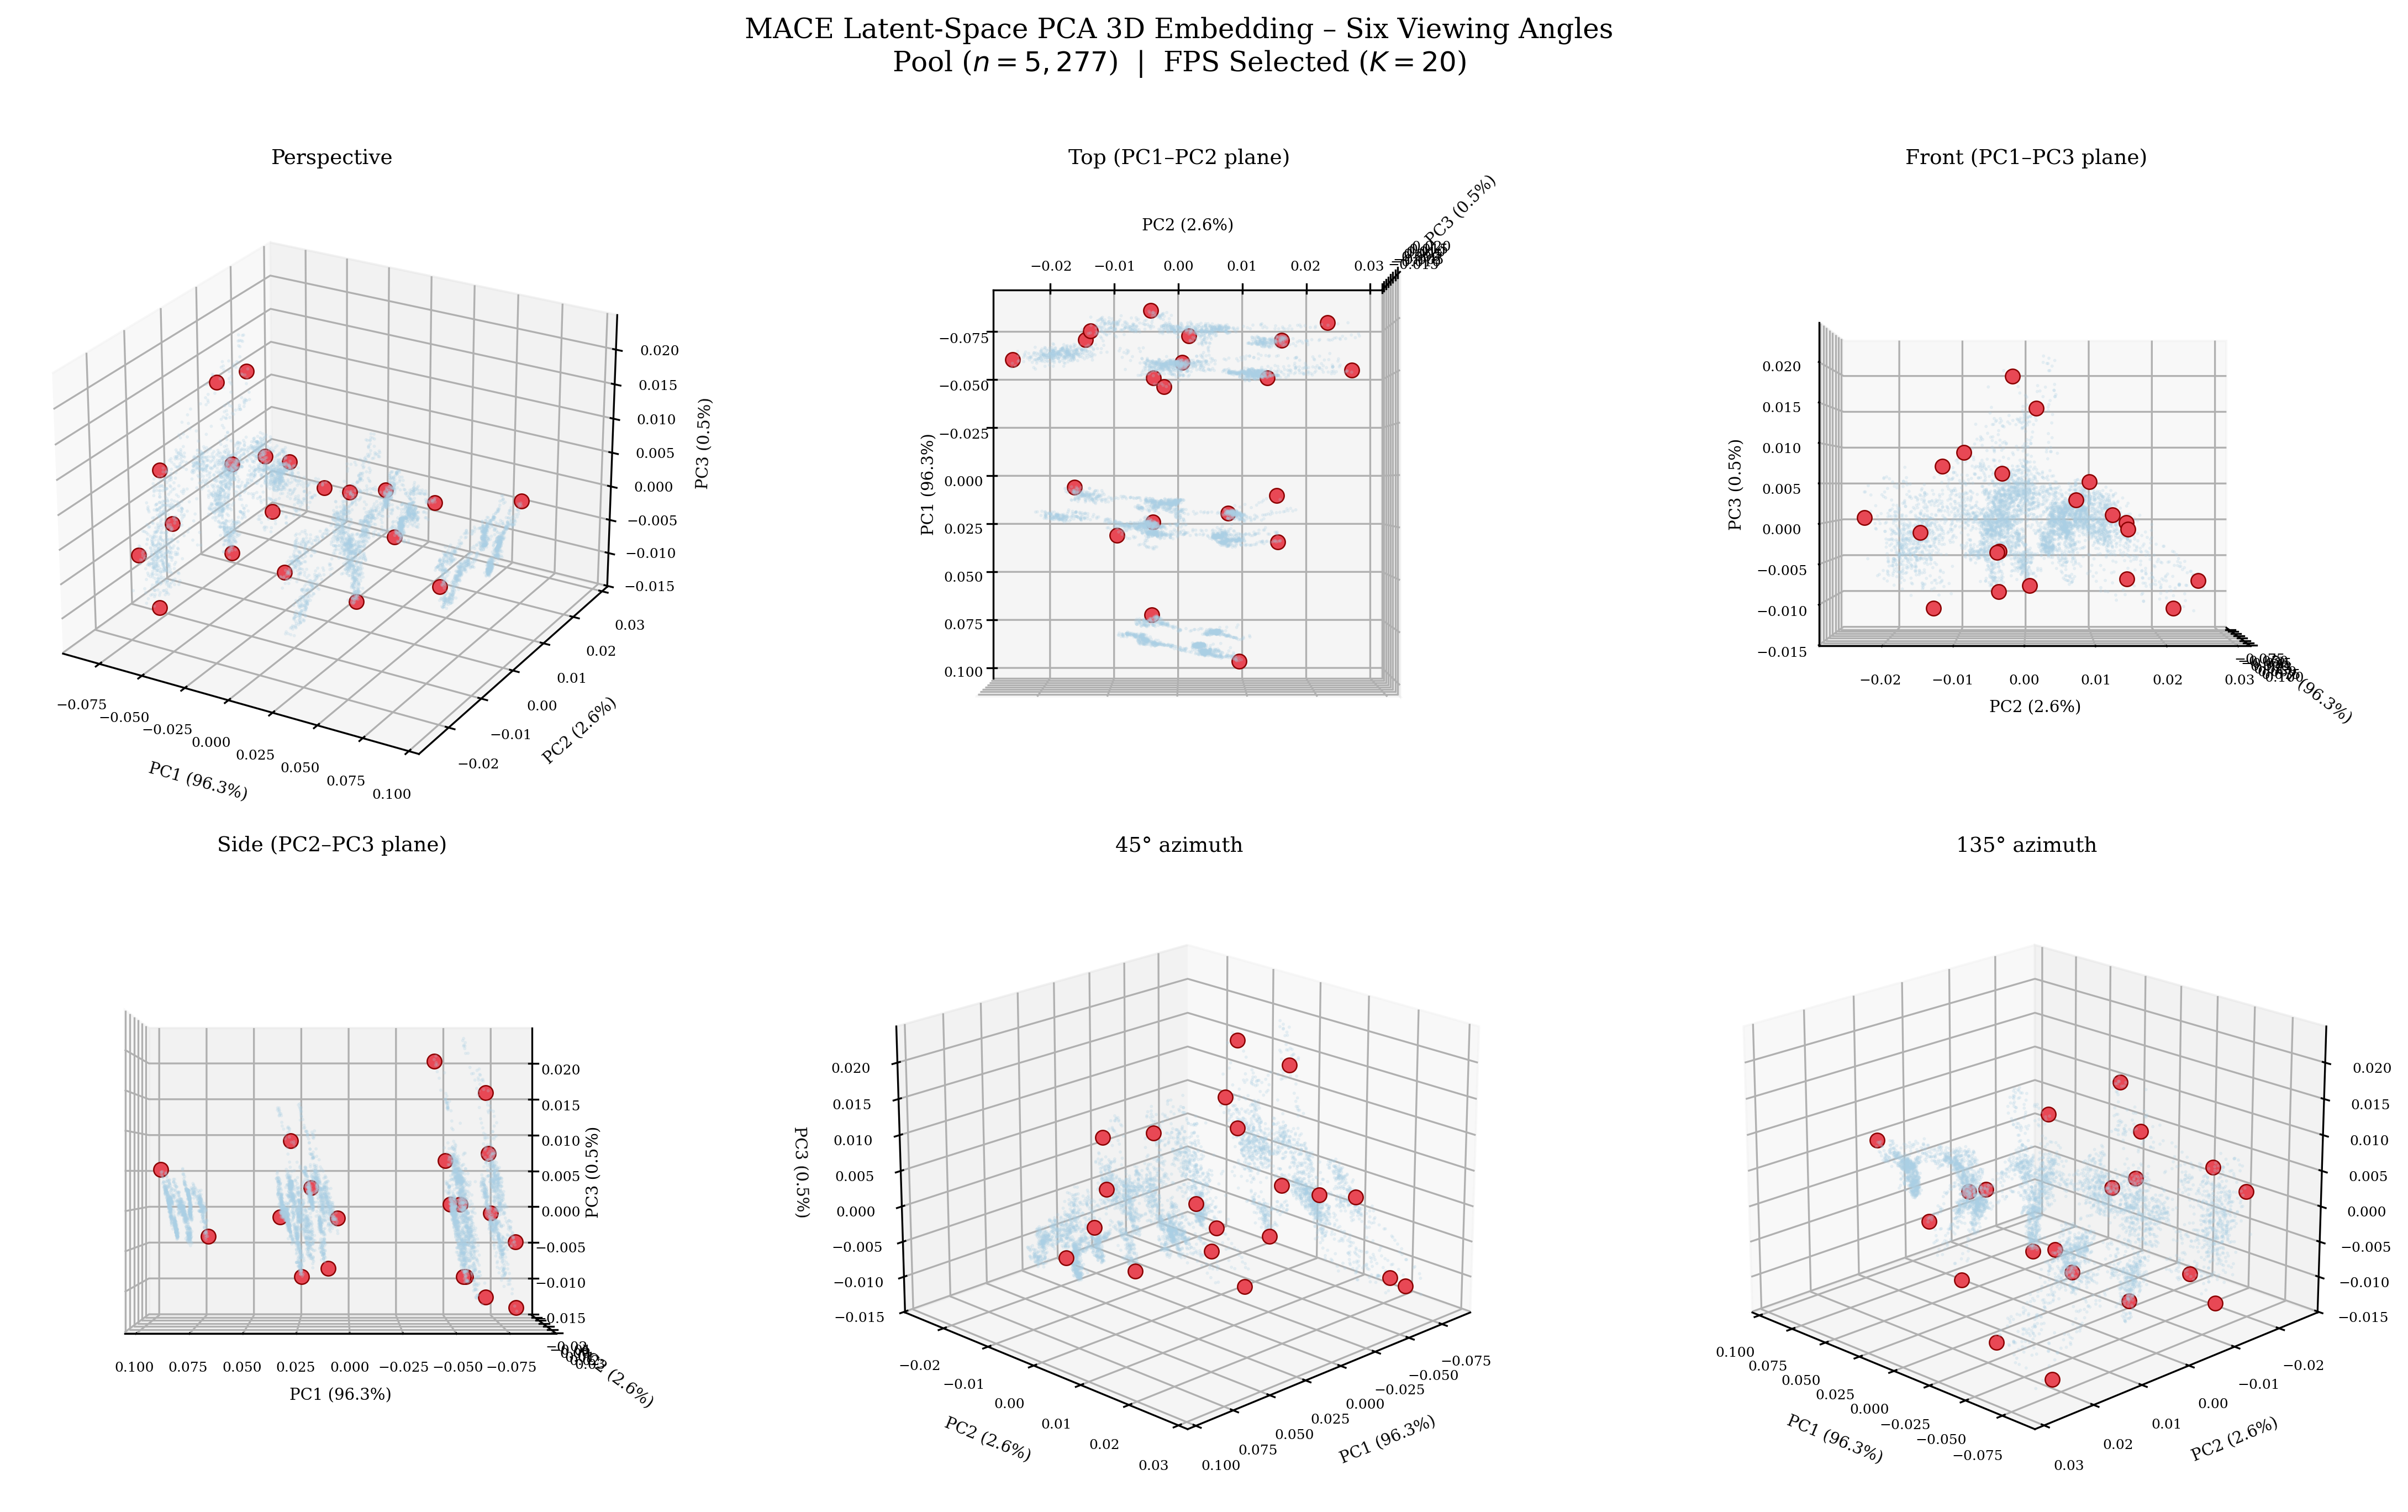
\includegraphics[width=0.9\textwidth]{fig_3d_emb_it0.png}
    \caption{3D perspectives of the PCA-reduced MACE latent space, demonstrating the spatial spread of the FPS-selected subset relative to the background structure pool.}
    \label{fig:fps_pca_3d}
\end{figure}

\subsection{Coverage Statistics of the Selected Latent Space}
\label{sec:coverage_stats}

To quantitatively assess the extent to which the Farthest Point Sampling selected structures (\(\mathcal{S}\), where \(K=20\)) uniformly span the pool's distribution (\(\mathcal{P}\), where \(N=5,297\)) in the latent space, a set of stringent coverage metrics was computed over the 32-dimensional principal component embeddings.

\subsubsection{Coverage Results}
Coverage metrics were computed as defined in Section~\ref{sec:coverage_stats_methods}. 
The FPS selection achieved a mean per-point coverage distance of 
$\bar{\delta}_k = 0.0093$ (median 0.0097), with a coverage radius of 
$\rho = 0.0176$. As shown in Figure~\ref{fig:coverage_metrics}, 95\% of pool 
structures fall within an embedding distance of $d = 0.0148$ of a selected 
structure, confirming that no significant region of the sampled configuration 
space was left unrepresented by the 20 selected structures.

\begin{figure}[htbp]
    \centering
    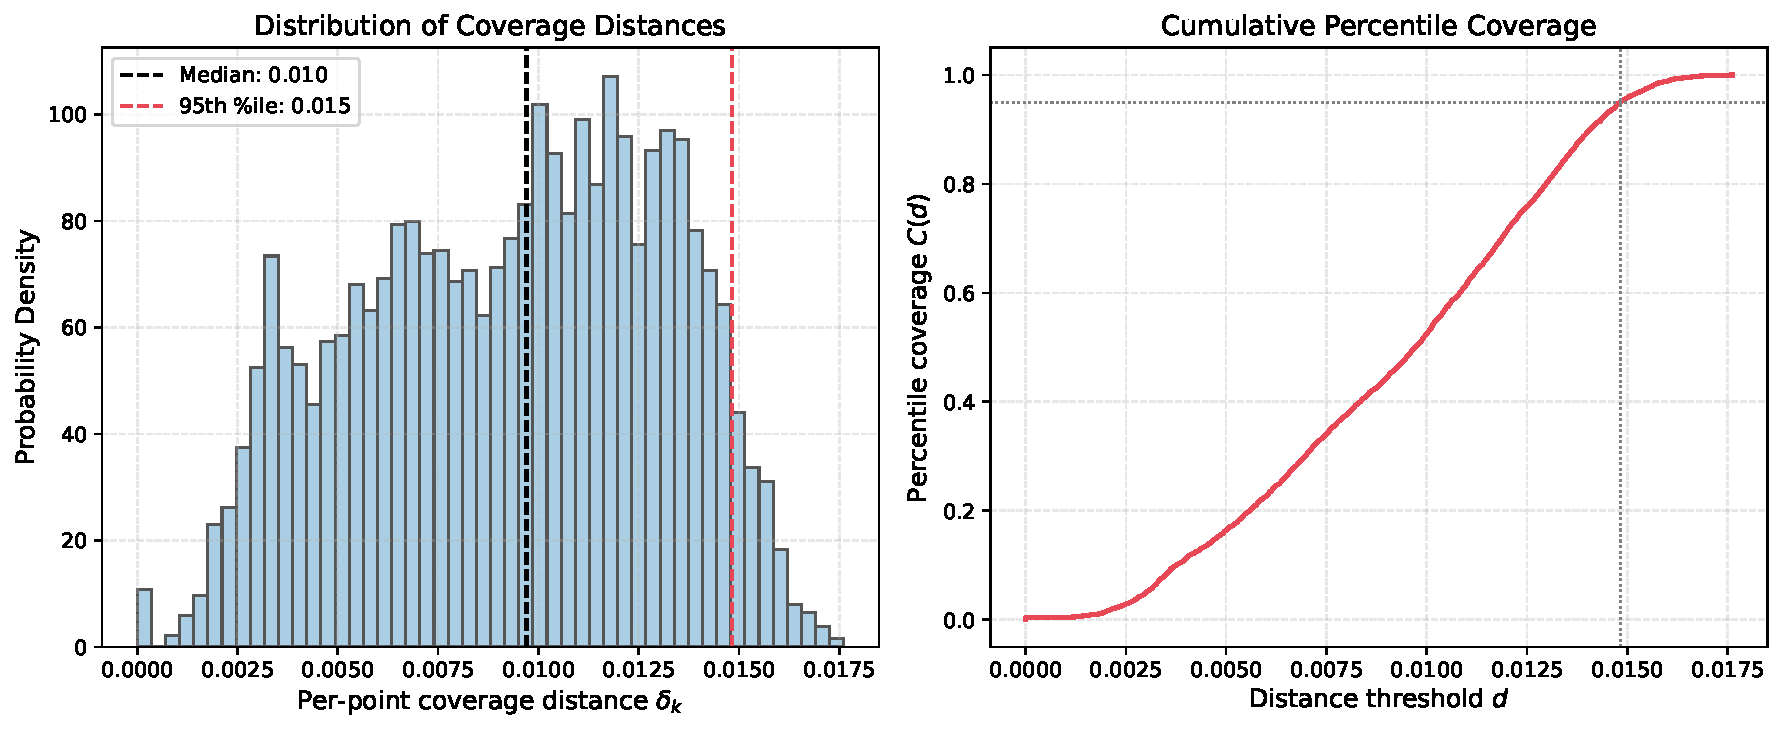
\includegraphics[width=0.9\textwidth]{coverage_statistics.pdf}
    \caption{(a) The probability density distribution of the per-point coverage distances \(\delta_k\) for the 5,297 pool structures. The median coverage distance (0.0097) and 95\textsuperscript{th} percentile boundary (0.0148) are annotated, confirming dense structural representation. (b) The Cumulative Percentile Coverage curve \(C(d)\), reaching 95\% closure at a tight threshold distance of \(d=0.0148\).}
    \label{fig:coverage_metrics}
\end{figure}

\begin{figure}[htbp]
\centering
\begin{subfigure}{0.48\linewidth}
    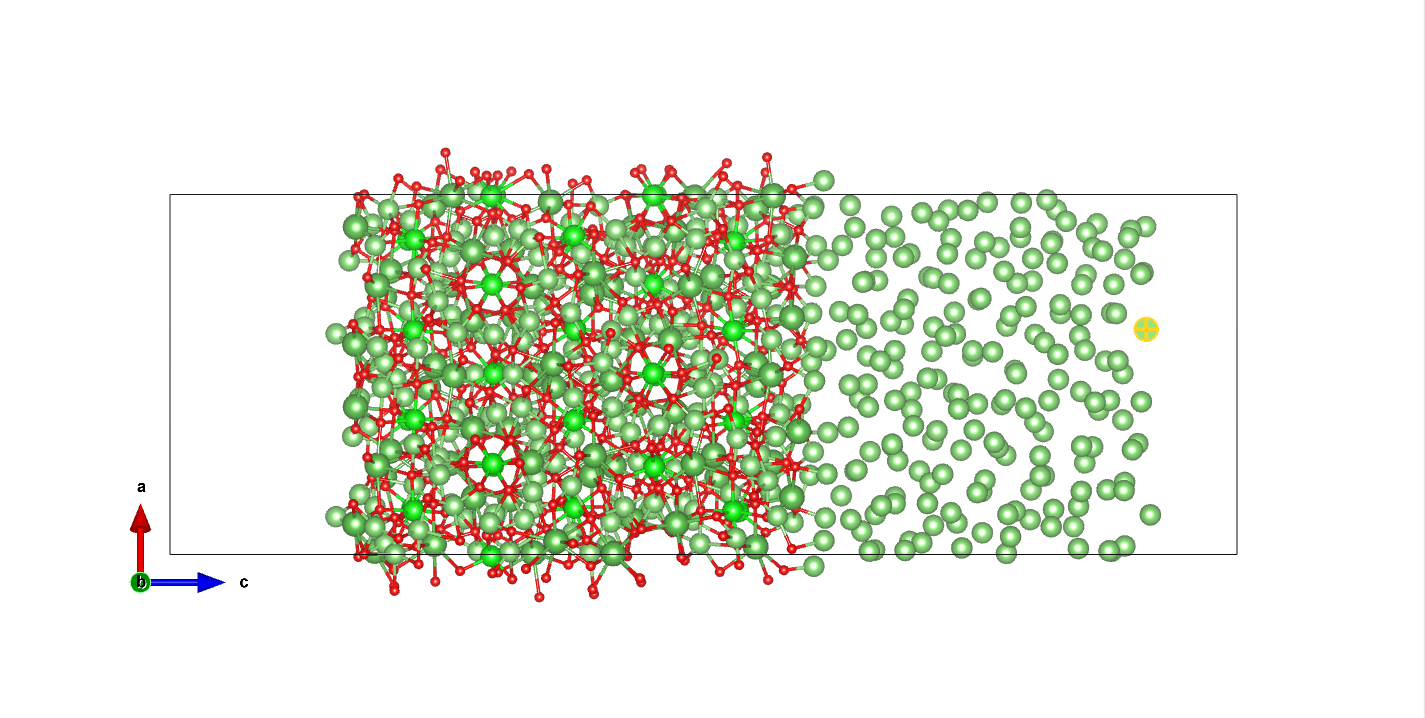
\includegraphics[width=\linewidth]{non_centered.png}
    \caption{Structure after MD with $\sim$5~\AA\ vacuum on Li metal side.}
    \label{fig:non_centered}
\end{subfigure}
\hfill
\begin{subfigure}{0.48\linewidth}
    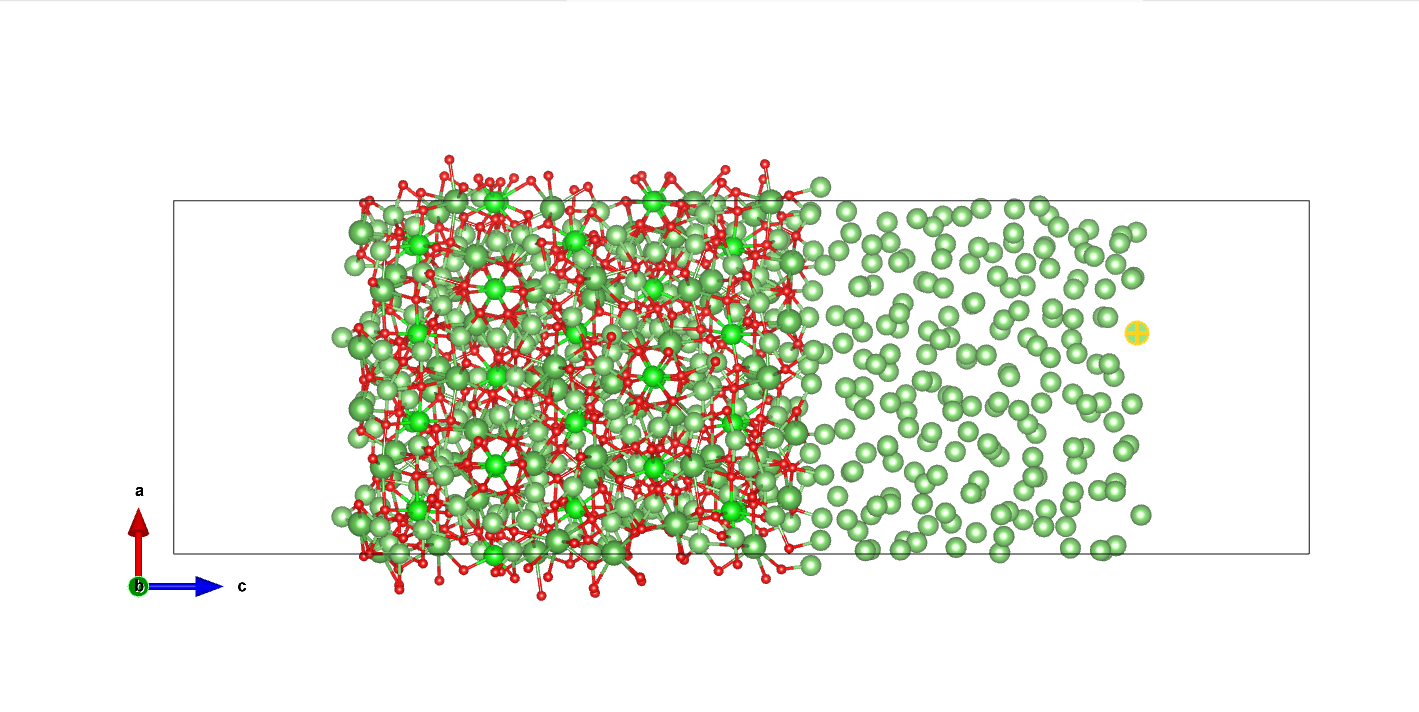
\includegraphics[width=\linewidth]{centered.png}
    \caption{Post-processed structure with 7.5~\AA\ vacuum added on each side.}
    \label{fig:centered}
\end{subfigure}
\caption{Interface structures before and after preprocessing for DFT labeling.
The increased vacuum spacing in (b) ensures proper decay of the electronic
wavefunction and eliminates spurious periodic-image interactions.}
\label{fig:centering_comparison}
\end{figure}

\subsubsection{Validation of Latent Space and Data Preparation}

Three consistency checks confirm the robustness of the FPS procedure. First, the 
minimum pairwise distance among selected structures (0.0180) exceeds the coverage 
radius (0.0176), confirming minimal redundancy within the selected set. Second, 
PCA projection introduces negligible geometric distortion, with mean relative 
distortion in pairwise distances of only 0.02\%. Third, centering structures and 
adding 7.5~\AA\ vacuum prior to DFT labeling produces embeddings differing by a 
mean $\ell_2$ distance of $1.24 \times 10^{-6}$ from the originals (cosine 
similarity $> 0.999999$), confirming that MACE embeddings encode intrinsic chemical 
environments rather than extrinsic geometric artifacts. All structures passed a 
minimum interatomic distance check of 1.7~\AA.

To facilitate DFT calculations, selected structures were centered and padded with 
7.5~\AA\ vacuum on each side along the surface normal, as shown in 
Figures~\ref{fig:non_centered} and~\ref{fig:centered}.
\subsection{Fine-Tuning of the MACE-OMAT Universal Model}

%% CHANGED: \Sec.~\ref{...} → \secref{sec:dft_labeling}
The initial set of $K=20$ structures selected via Farthest Point Sampling (FPS) was labeled using DFT-FE, as described in \secref{sec:dft_labeling}. These structures constitute the first active learning dataset used for finetuning the pretrained MACE-OMAT universal model.

\paragraph{Train--validation splitting --}
\label{para:it0_splitting}
To ensure robust evaluation across systems of varying sizes, the dataset was stratified based on the number of atoms in each structure. Four buckets were defined: 400--600, 650--800, 850--1050, and 1100--1400 atoms. For each split, 16 structures were used for training and 4 for validation.

This multi-split strategy is particularly important in the present small-data regime, where model performance can be sensitive to the specific choice of training and validation structures. By multiple stratified splits and selecting the best-performing model, we mitigate variance due to data partitioning and obtain a more reliable estimate of model generalization.

To reduce sensitivity to a particular train--validation split and obtain statistically meaningful performance estimates, 20 independent stratified splits were generated. A separate model was trained on each split.

The final reported model corresponds to the best-performing instance, selected based on a combination of low energy and force errors on the validation set, together with consistent agreement between training and validation metrics, indicating stable generalization without evidence of overfitting or underfitting.

\paragraph{Training protocol --}
Finetuning was performed using low-rank adaptation (LoRA) with rank $r=5$ and scaling parameter $\alpha = 1.0$. Training was carried out for up to 260 epochs with early stopping based on validation loss. The best-performing model was selected from epoch 240.

\paragraph{Model performance --}
The finetuned model achieves low and consistent errors on both training and validation sets:

\begin{center}
\begin{tabular}{lccc}
\hline
Config type & RMSE (E) [meV/atom] & RMSE (F) [meV/\AA] & Relative F RMSE (\%) \\
\hline
Train & 4.6 & 51.5 & 7.97 \\
Validation & 4.7 & 50.5 & 9.07 \\
\hline
\end{tabular}
\end{center}

The close agreement between training and validation errors indicates the absence of significant overfitting. In particular, the force RMSE remains stable across splits, which is critical for reliable structural relaxation and molecular dynamics simulations.

\begin{figure}
    \centering
    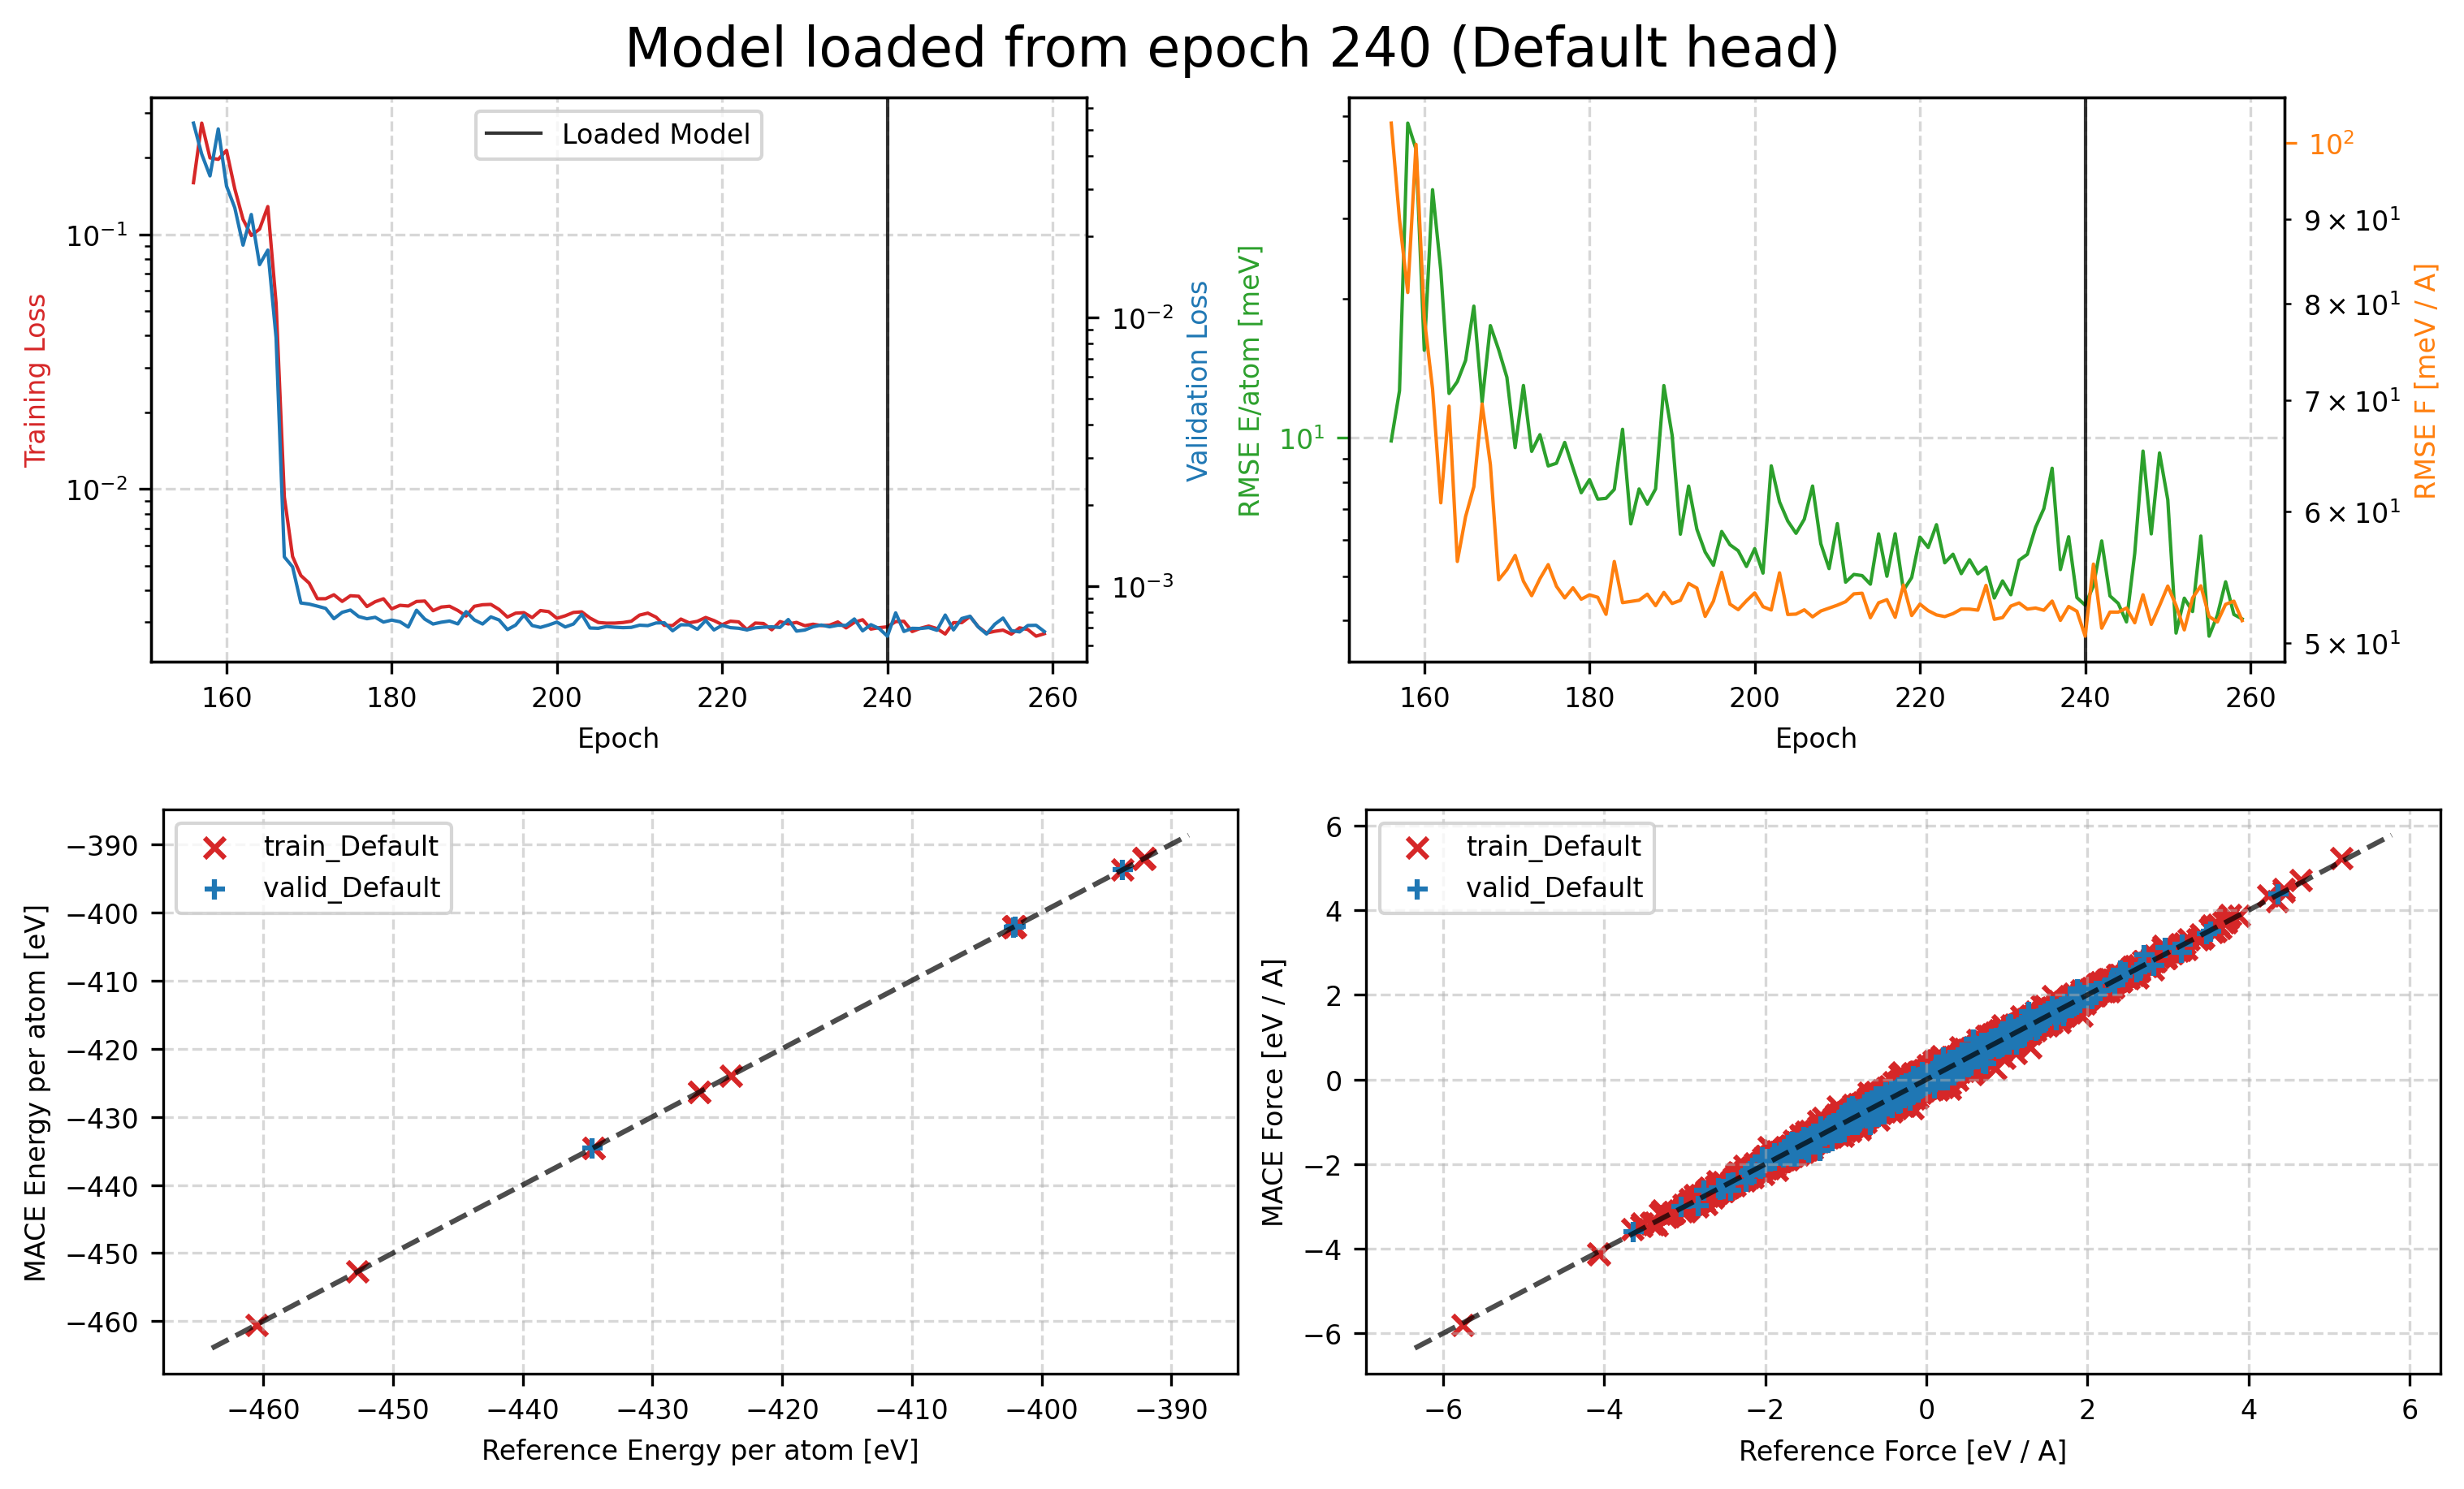
\includegraphics[width=\linewidth]{it0_finetuning_plot.png}
    \caption{Training and validation curves for the Iteration~0 LoRA finetuning run.
    Top row: total loss as a function of epoch for both the training and validation
    sets. Bottom row: energy RMSE (meV/atom) and force RMSE (meV/\AA) as a function
    of epoch. The close alignment of training and validation curves throughout confirms
    stable generalization without overfitting.}
    \label{fig:it0_finetuning_plots}
\end{figure}

\paragraph{Convergence behavior --}
Figure~\ref{fig:it0_finetuning_plots} shows the training and validation loss curves, along with the evolution of energy and force RMSE during training. Both loss and RMSE decrease rapidly in the initial stages and stabilize after approximately 180 epochs. The absence of divergence between training and validation curves confirms stable optimization and good generalization.

\paragraph{Energy and force correlation --}
Scatter plots comparing predicted and reference energies and forces demonstrate excellent agreement across both training and validation datasets. The predictions closely follow the ideal $y=x$ relationship, with no systematic bias or large outliers observed.

Overall, these results indicate that finetuning with a small, diverse FPS-selected dataset is sufficient to significantly improve model accuracy while maintaining generalization across heterogeneous interface configurations. The MACE-OMAT universal had an initial RMSE of Energy per atom at 606.79 meV while RMSE for Forces were 135.60 meV/\AA, which were reduced to $4.7$~meV/atom (energy) and $50.5$~meV/\AA\ (forces)
on the validation set. This finetuned model is called the \textbf{MACE-Iteration-0} model.

\section{Iteration~1 Finetuning}
\label{sec:results_it1}

Following the Iteration 0 model, a second active learning cycle was performed to extend coverage of the interface configuration space.

\subsection{MD Sampling and Dataset Construction}

Molecular dynamics simulations were carried out using the Iteration 0 model on the same 13 relaxed interface configurations used to construct the initial training set. Simulations were run at two temperatures, 550~K and 1100~K. Snapshots were extracted every 100 MD steps (compared to every 25 steps in
Iteration~0) to reduce pool size while maintaining adequate configurational
diversity, given that the Iteration~0 model drives less aggressive thermal
excursions than the universal MACE-OMAT model. Configurations with atomic overlaps (minimum interatomic distance $<1.6$~\AA) were removed, leaving $\sim$1,300 pool structures. Each snapshot was centred and padded with vacuum using the same preprocessing pipeline applied in Iteration 0.

%% CHANGED: Burov2021 → Burov2024LiLLZOChargeTransfer
To supplement regions of configuration space that MD cannot reach by construction (see Section~\ref{sec:it1_external}), 20 additional interface structures drawn from \citeauthor{Burov2024LiLLZOChargeTransfer}~\cite{Burov2024LiLLZOChargeTransfer} were appended to the pool before sampling. The combined pool therefore contains $\sim$1,320 structures in total.

\subsection{Latent Space Coverage Analysis}

Latent embeddings were extracted from the Iteration 0 MACE model for all pool structures, $\ell_2$-normalised, and projected into the 32-dimensional PCA subspace used throughout this pipeline (capturing $\geq 99.9\%$ of total structural variance).

For each pool structure $k$, the minimum Euclidean distance to the 16 training seed structures $\mathcal{T}$ was computed:
\begin{equation}
    \delta_k = \min_{\mathbf{Z}_s \in \mathcal{T}} \|\mathbf{Z}_k - \mathbf{Z}_s\|_2
\end{equation}

The resulting coverage statistics are summarised in Table~\ref{tab:it1_coverage}. The worst-case structure --- a Li(100)/LLZO(011-La) snapshot at 550~K --- sits at $\delta = 0.0204$, at the 99.9th percentile of the pool distribution. The cumulative coverage function, shown in Figure~\ref{fig:it1_cdf}, reaches $C(d) = 0.95$ at $d = 0.0183$, confirming that the MD trajectories explore configurations beyond the Iteration 0 training boundary while remaining physically coherent.

\begin{table}[htbp]
\centering
\caption{Per-point coverage distance statistics for the Iteration 1 pool ($n \approx 1{,}320$) relative to the 16 training seeds $\mathcal{T}$.}
\label{tab:it1_coverage}
\begin{tabular}{lc}
\hline
Statistic & Value \\
\hline
Mean $\bar{\delta}_k$                    & 0.0132 \\
Median $\delta_{50}$                     & 0.0135 \\
90th percentile $\delta_{90}$            & 0.0175 \\
95th percentile $\delta_{95}$            & 0.0183 \\
Coverage radius $\rho = \max_k \delta_k$ & 0.0204 \\
\hline
\end{tabular}
\end{table}

\begin{figure}[htbp]
    \centering
    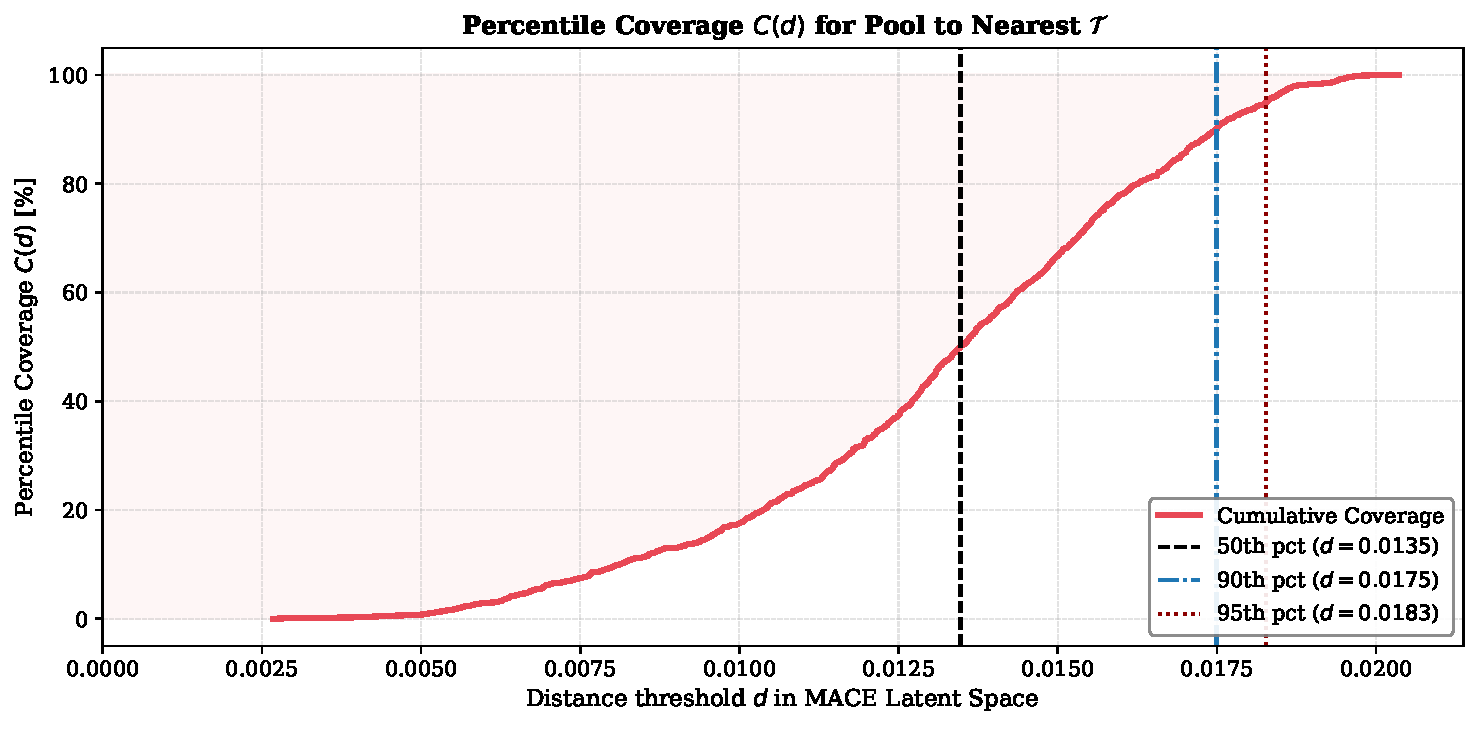
\includegraphics[width=0.8\textwidth]{it1_split17_coverage_percentile_cdf.pdf}
    \caption{Cumulative coverage $C(d)$ for the Iteration 1 pool. Vertical lines mark
    the 50th ($d=0.0135$), 90th ($d=0.0175$), and 95th ($d=0.0183$) percentiles.
    The coverage radius $\rho = 0.0204$ is the worst-case distance from any pool
    structure to the nearest training seed.}
    \label{fig:it1_cdf}
\end{figure}

\subsection{Structure Selection via FPS and Super-FPS}

\paragraph{Stage 1: Coarse FPS selection --}
Farthest Point Sampling was first applied to the full Iteration~1 pool in the
PCA-reduced MACE latent space, using the existing training set
$\mathcal{T}$ as the seed set. This produced an intermediate set of 20
diverse candidate structures. Because the seed set already contains the
previously labeled configurations, the selected candidates correspond to
regions of latent space that are poorly represented by the current model
training data.
\paragraph{Stage 2: Super-FPS refinement --}
A second FPS pass was then applied to the 20 coarse candidates, again using
the current training set as the seed set, to select the final $K=6$
structures for DFT labeling. This refinement step removes redundancy among
the coarse FPS candidates and retains only those structures that are most
complementary to the existing training set in latent space. After selection,
coverage statistics were computed by assigning each pool structure to its
nearest representative among the training set and the newly selected
Super-FPS structures.
\subsection{Selection Characteristics}

To quantify the representative power of each selected structure, we assigned every point in the $\sim$1300-structure pool to its closest neighbor in the combined set of training seeds ($\mathcal{T}$) and the six new Super-FPS selections. In this context, the ``coverage'' of a Super-FPS structure is simply the number of pool snapshots that are closer to it than to any other known structure in the latent space. This partitions the newly generated MD data into local structural clusters, with each Super-FPS selection acting as the representative centroid for its cluster.

Using this definition, we found that the high-temperature configurations are responsible for the vast majority of out-of-distribution exploration. Among the four MD-drawn selections, the three 1100~K picks (Ranks 1, 2, and 4) stand as the closest structural proxies for a combined 681 of the $\sim$1,300 MD snapshots (52.4\%). Rank 1 alone --- a heavily distorted Li(111)/LLZO(110-Zr) frame --- serves as the representative centroid for 300 distinct snapshots, making it the focal point of the largest unlabelled cluster in the entire Iteration 1 pool. The single 550~K pick (Rank 6) sits adjacent to a smaller grouping, covering a further 179 structures.

In aggregate, the six Super-FPS structures pull 922 of the $\sim$1,320 pool structures (69.8\%) into their local neighbourhoods. The remaining $\sim$30\% of the pool consists of near-equilibrium fluctuations that correctly fall back within the coverage radii of the existing Iteration 0 training seeds.

Figure~\ref{fig:it1_super_fps} shows the final six selections annotated directly in the latent space, illustrating how they systematically anchor these disconnected clusters.

\begin{figure}[htbp]
    \centering
    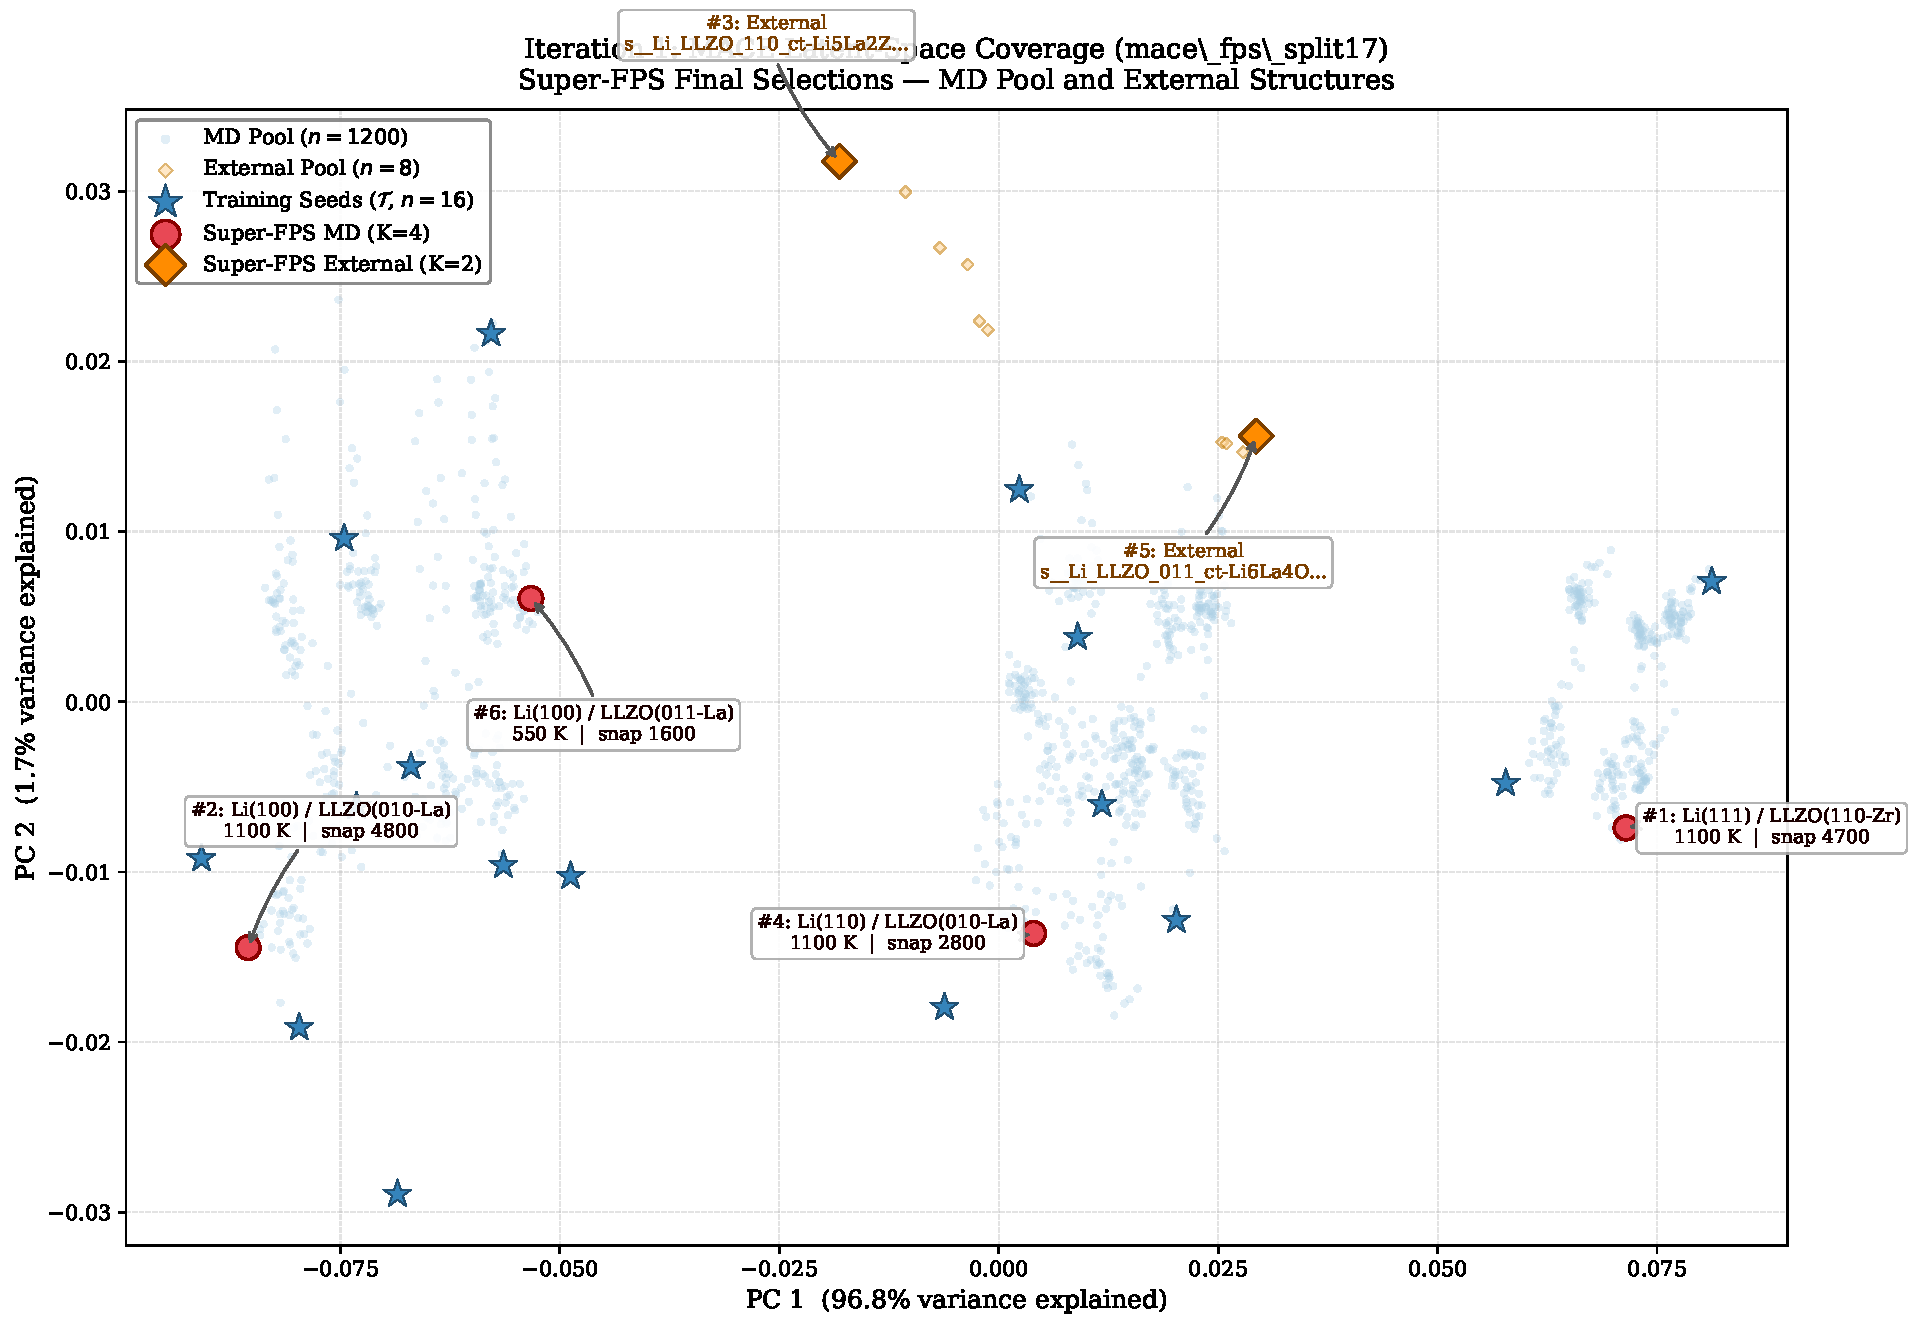
\includegraphics[width=\textwidth]{it1_split17_super_fps_2d.pdf}
    \caption{2D PCA projection of the Iteration 1 pool (pale blue), training seeds
    $\mathcal{T}$ (blue stars), and the six Super-FPS final selections. Red circles
    denote MD-drawn structures; orange diamonds denote external structures. The two
    external picks (Ranks 3 and 5) occupy the isolated rightmost cluster, confirming
    they lie outside the MD-sampled region.}
    \label{fig:it1_super_fps}
\end{figure}

\paragraph{Inclusion of external structures --}
\label{sec:it1_external}
%% CHANGED: Burov2021 → Burov2024LiLLZOChargeTransfer throughout
The two external structures (Ranks 3 and 5) are interface geometries inspired from
\citeauthor{Burov2024LiLLZOChargeTransfer}~\cite{Burov2024LiLLZOChargeTransfer} with compositions not present in the training set,
such as a Li/LLZO(110) interface with a Li$_5$La$_2$Zr$_4$O$_8$ bulk termination.
Their distances to the nearest training seed ($\delta = 0.040$ and $0.030$) are roughly
$2\times$ and $1.5\times$ beyond the MD pool maximum of $\rho = 0.0204$, meaning no MD
snapshot reached their vicinity regardless of temperature or run length. This is a
structural limitation of MD sampling: because the trajectories are propagated by the
Iteration 0 model, they can only explore configurations dynamically accessible from the
training structures. Interface stacking sequences the model has never encountered cannot
emerge from MD alone. Including these two structures in the DFT batch therefore fills
gaps that would otherwise persist into Iteration 2.

\subsection{Summary of Iteration 1 Selection}

The Iteration~1 selection adds six DFT-labeled structures through the
two-stage Super-FPS procedure. The selected configurations are well separated
in the MACE latent space and complement the structures already present in the
training set. As shown in Fig.~\ref{fig:it1_super_fps}, the selected structures
include both MD-sampled configurations and two external interface geometries
that lie outside the MD-sampled region. The cumulative coverage profile in
Fig.~\ref{fig:it1_cdf} further shows that the selected structures improve the
representation of the newly sampled configuration space. Overall, the
Iteration~1 selection provides a compact and non-redundant set of configurations
for the next finetuning step.

\subsection{Fine-Tuning of the Iteration 1 Model}

%% CHANGED: \Sec.~\ref{...} → \secref{sec:dft_labeling}
The structures selected via the Iteration 1 active learning loop were labeled using DFT-FE as described in \secref{sec:dft_labeling}. These newly labeled configurations were combined with the previous dataset to further refine the MACE-OMAT universal model.

\paragraph{Train--validation splitting --}
The same stratified splitting strategy described in 
Section~\ref{para:it0_splitting} was applied to the combined dataset, with 
20 independent splits (20 training, 6 validation) and selection of the best-performing model based on 
validation metrics. 

\paragraph{Training protocol --}
Finetuning was performed using low-rank adaptation (LoRA) with rank $r=5$ and scaling parameter $\alpha = 1.0$. Training was carried out for up to 300 epochs with early stopping based on validation loss. The best-performing model was selected at epoch 109.

\paragraph{Training dynamics --}
The training curves for Iteration 1 are shown in Figure~\ref{fig:it1_finetuning_plots}. The loss decreases smoothly during training, with both training and validation curves remaining closely aligned throughout. No discontinuities or instabilities are observed in the optimization trajectory.

Energy errors converge rapidly to low values, while force errors exhibit a slower but stable convergence. This behaviour is expected, as forces represent local derivatives of the energy and are inherently more sensitive to structural variations.

\paragraph{Model performance --}
The final performance of the Iteration 1 model is summarised below:

\begin{center}
\begin{tabular}{lccc}
\hline
Config type & RMSE (E) [meV/atom] & RMSE (F) [meV/\AA] & Relative F RMSE (\%) \\
\hline
Train & 4.6 & 54.5 & 8.39 \\
Valid & 3.7 & 55.4 & 9.28 \\
\hline
\end{tabular}
\end{center}

The close agreement between training and validation errors indicates stable generalization, with no evidence of overfitting or underfitting. The force RMSE remains consistent across splits, confirming the robustness of the model in capturing local atomic interactions.

\begin{figure}
    \centering
    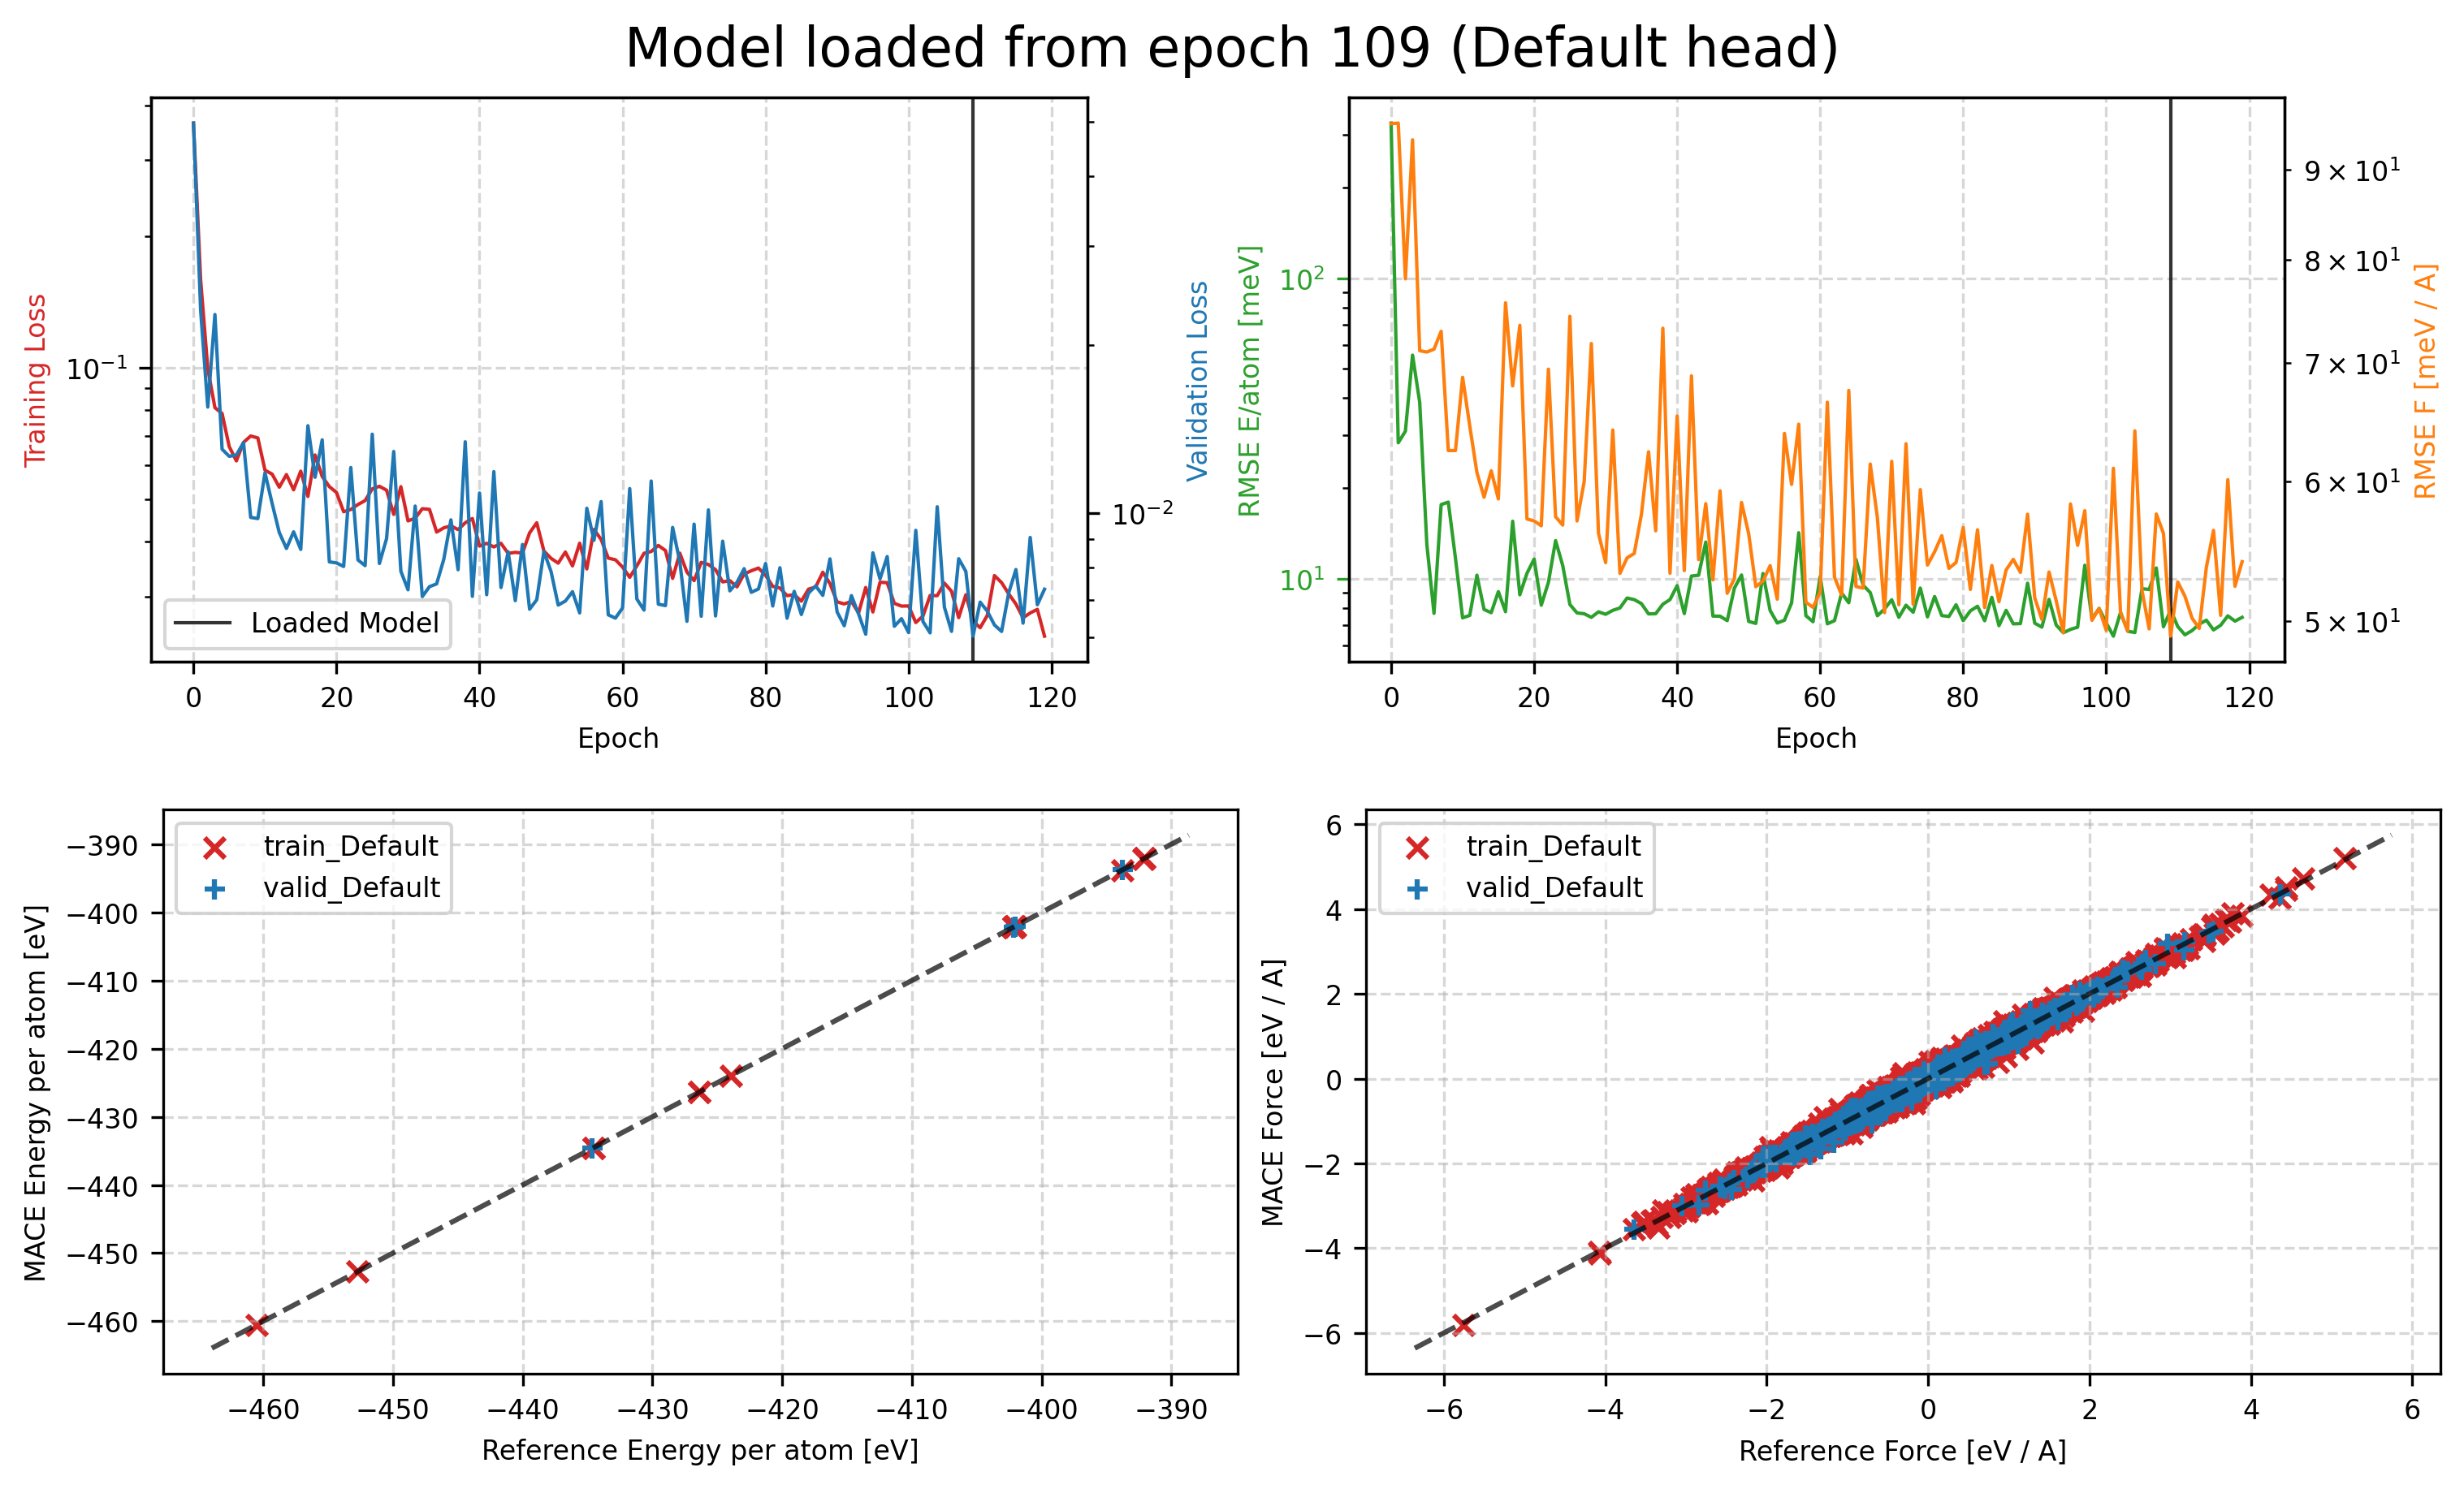
\includegraphics[width=\linewidth]{it1_ft_plt.png}
    \caption{Training and validation loss, along with energy and force RMSE as a function of epoch for the chosen Iteration 1 model. The smooth convergence and close agreement between training and validation curves indicate stable optimization without overfitting. Parity plots for energy and forces demonstrate strong agreement between predicted and reference values.}
    \label{fig:it1_finetuning_plots}
\end{figure}

\paragraph{Energy and force correlation --}
Parity plots comparing predicted and reference energies and forces (Figure~\ref{fig:it1_finetuning_plots}) show excellent agreement along the ideal $y=x$ line for both training and validation datasets. No systematic bias or large deviations are observed.

Overall, these results demonstrate that the Iteration 1 active learning cycle successfully improves the model while maintaining stable training dynamics and strong generalization across diverse interface configurations.

%% CHANGED: added label for cross-reference
\section{Performance on Unseen and Out-of-Distribution Structures}
\label{sec:ood}

To evaluate the generalization capability of the trained models beyond the active learning distribution, we assess their performance on a deliberately constructed set of unseen and out-of-distribution (OOD) interface structures.

A total of 8 test structures were considered (Table~\ref{tab:ood_results}). Of these, 5 structures were relaxed using the Iteration 1 model, while the remaining 3 were kept in their unrelaxed configurations to probe robustness under non-equilibrium geometries. Importantly, these structures were constructed using a different source of LLZO geometries compared to the training data. Specifically, LLZO slabs were derived from the interface geometries of
\citeauthor{Burov2024LiLLZOChargeTransfer}, which feature different Li-site
occupancy patterns, lattice parameters ($a = b \neq c$), and surface
termination compositions relative to the tetragonal LLZO source structures
of \citeauthor{Canepa2018LLZO} used throughout training. This introduces a systematic shift in local atomic environments, coordination patterns, and lattice distortions, making these structures inherently challenging for the model to capture.

\paragraph{Why the Canepa- and Burov-derived slabs differ --}
Although the bulk LLZO backbone remains recognizable in both datasets, the local
polyhedral environments differ because the two studies probe different parts of
LLZO configuration space. The slabs used throughout training are derived from the
free-surface study of \citeauthor{Canepa2018LLZO}, which targets neutral
thermodynamic surface minima and therefore primarily reflects surface termination,
Li/O reconstruction, and segregation physics. By contrast, the OOD structures
derived from \citeauthor{Burov2024LiLLZOChargeTransfer} correspond to a more
redox-flexible and interface-perturbed regime, where the surface geometry is
already influenced by charge compensation and proximity to Li metal.

As a result, the structural differences between the two sets are physically
meaningful rather than incidental. In the Canepa-derived slabs, the La--Zr--O
framework remains comparatively close to a free-surface minimum, while the main
reconstructions occur in the outer Li and O layers. In the Burov-derived slabs,
the same polyhedral families are coupled to interface-driven electronic
reorganization: ZrO$_6$ octahedra can act as redox-active units, oxygen can
participate in oxidation compensation, and stronger Li--O interactions emerge
near the interface. This makes the Burov structures an intentionally stringent
OOD test, since they probe local environments that are structurally and
chemically distinct from those represented in the Canepa-based training pool.

This distinction is also important physically. The Canepa slabs are best viewed
as descriptors of free-surface thermodynamics and lithium segregation, whereas
the Burov slabs are more representative of interface redox, Li--O mediated
adhesion/reconstruction, and charge-transfer physics under Li-metal contact.

\begin{figure}[htbp]
\centering
\begin{subfigure}{0.48\textwidth}
    \centering
    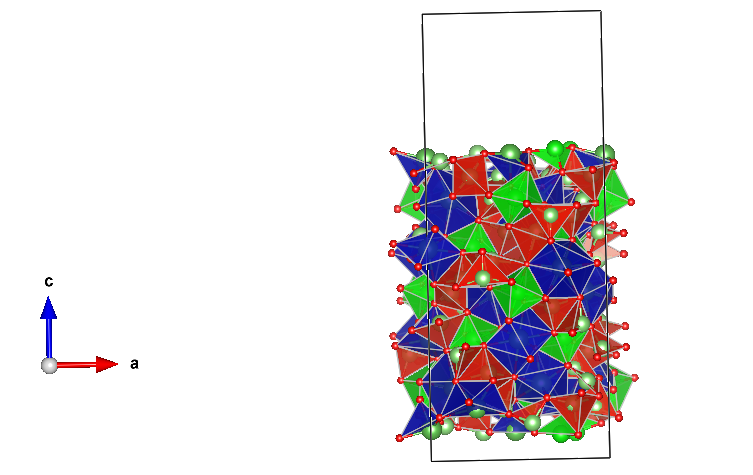
\includegraphics[width=\linewidth]{burov_type_slab.png}
    \caption{Canepa-type LLZO slab. The structure is closer to a neutral free-surface thermodynamic minimum.}
    \label{fig:canepa_type_slab}
\end{subfigure}
\hfill
\begin{subfigure}{0.48\textwidth}
    \centering
    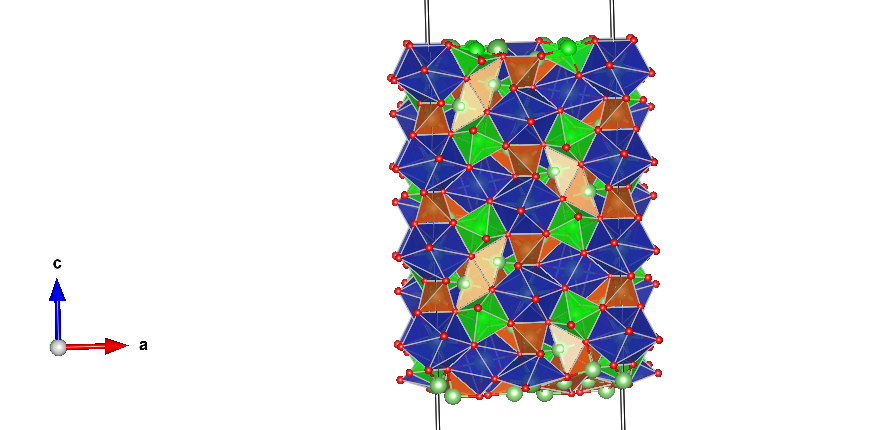
\includegraphics[width=\linewidth]{canepa_type_slab.png}
    \caption{Burov-type LLZO slab. The local coordination environment reflects a more redox-flexible, interface-perturbed structural regime.}
    \label{fig:burov_type_slab}
\end{subfigure}
\caption{Comparison of the two LLZO slab types used in this work. Although the bulk garnet backbone remains similar, the local motifs differ because the Canepa-derived structures represent free-surface minima, whereas the Burov-derived structures reflect interface-perturbed and redox-active local environments.}
\label{fig:canepa_burov_comparison}
\end{figure}
% the figures are correct, by accident file-names are swapped, labels are correct as well.
\paragraph{Evaluation metric: cohesive energy --}
Direct comparison of total energies across models is not meaningful due to differences in reference energy scales. All DFT reference calculations were performed using DFT-FE with SPMS pseudopotentials, whereas the pretrained MACE-OMAT universal model is aligned with VASP-PBE reference energies.

To enable consistent comparison, cohesive energies were computed as:
\begin{equation}
E_{\mathrm{coh}} = \frac{E_{\mathrm{tot}} - \sum_i n_i E_i^{\mathrm{atom}}}{N}
\end{equation}

For the finetuned models, the single-atom reference energies were explicitly incorporated during training via the $E_0$ offsets. These reference energies were computed using DFT-FE with SPMS pseudopotentials, yielding the following values (in eV): Li: $-190.7590$, O: $-442.9889$, Zr: $-1380.1817$, and La: $-958.0774$.

In contrast, the MACE-OMAT universal model is calibrated to VASP-PBE reference energies using standard VASP pseudopotentials. Accordingly, cohesive energies for the universal model were computed using VASP-PBE single-atom reference energies (Li: $-0.0865$, La: $-0.3840$, Zr: $-1.4709$, O: $-0.1665$ eV), ensuring alignment of its intrinsic energy scale.

This adjustment provides a conservative comparison by effectively correcting for differences in absolute energy references between DFT-FE and VASP-based models.

\paragraph{Results and discussion --}
The results are summarized in Table~\ref{tab:ood_results}. Across all structures, both finetuned models outperform the MACE-OMAT universal model in cohesive energy and force predictions, with Iteration 1 showing the best overall performance.

\begin{table}[htbp]
\centering
\caption{Performance on unseen and out-of-distribution (OOD) interface structures. Structure IDs are arbitrary labels used for cross-referencing within this table. CE Err is reported in meV/atom and Force error is reported in meV/\AA.}
\label{tab:ood_results}

\resizebox{\textwidth}{!}{
\begin{tabular}{cccccccc}
\hline
Structure ID & $N_{\text{atoms}}$ & CE Err (It0) & CE Err (It1) & CE Err (OMAT) & F RMSE (It0) & F RMSE (It1) & F RMSE (OMAT) \\
\hline
2 & 544 & 2.87 & 2.55 & -16.04 & 59.79 & 43.96 & 113.98 \\
6 & 544 & 7.27 & 6.33 & -14.27 & 110.35 & 71.51 & 90.26 \\
1 & 776 & -1.45 & -1.01 & -16.59 & 180.34 & 96.22 & 114.03 \\
7 & 816 & 2.08 & 0.36 & -18.36 & 76.38 & 105.11 & 201.85 \\
0 & 544 & -5.56 & 2.59 & -15.59 & 242.78 & 106.69 & 111.64 \\
4 & 776 & 2.82 & 1.81 & -15.91 & 101.22 & 115.78 & 179.54 \\
5 & 544 & 2.85 & 4.98 & -13.25 & 171.80 & 136.49 & 114.61 \\
3 & 776 & -4.98 & -0.30 & -13.35 & 199.44 & 151.66 & 127.31 \\
\hline
\textbf{RMSE} & -- & \textbf{4.17} & \textbf{3.21} & \textbf{15.51} & \textbf{155.16} & \textbf{108.27} & \textbf{136.44} \\
\hline
\end{tabular}
}
\end{table}

\paragraph{Key observations --}
\begin{itemize}
    \item \textbf{Improved generalization:} Both finetuned models significantly outperform the universal model on OOD structures.

    \item \textbf{Iteration improvement:} Iteration 1 consistently reduces both energy and force errors compared to Iteration 0.

    \item \textbf{Systematic bias in universal model:} The universal model shows large systematic deviations in cohesive energy, even after reference alignment.

    \item \textbf{Force prediction robustness:} Force RMSE is substantially reduced in finetuned models, particularly for relaxed structures.
\end{itemize}

Overall, these results demonstrate that targeted finetuning substantially improves robustness and accuracy in challenging interface environments, enabling reliable predictions even in regimes far from the training distribution.

\paragraph{Failure cases and limitations --}
While the finetuned models demonstrate strong overall performance, they are not uniformly superior across all metrics. In particular, there exist isolated cases (e.g., Structure IDs 5 and 3 in Table~\ref{tab:ood_results}) where the cohesive energy errors are small, but the force errors are higher than those of the MACE-OMAT universal model.

This behaviour highlights an important limitation of the current training regime. Energy and force predictions, although related through differentiation, do not necessarily improve uniformly during finetuning, especially in small-data regimes. The model can learn to reproduce the energy landscape locally while still exhibiting inaccuracies in its gradients, particularly in regions that are sparsely sampled or structurally distinct from the training distribution.

These failure cases are most pronounced for configurations with atypical local environments or incomplete relaxation, where force sensitivity to small geometric perturbations is high. In contrast, the universal model, having been trained on a significantly broader and more diverse dataset, can retain better force generalization in such edge cases.

This observation reinforces the importance of explicitly evaluating both energy and force metrics when assessing MLIP performance. It also suggests that further improvements may require either (i) targeted sampling of such high-error regions through additional active learning iterations, or (ii) rebalancing of energy--force loss weighting during training to better constrain force predictions in OOD regimes.

%% CHANGED: added label and restructured validation context
\subsection{Bulk cohesive-energy validation for Li and LLZO}

Before evaluating interface energetics, we assessed whether the models reproduce the cohesive energetics of the parent bulk phases, namely bcc Li metal and bulk LLZO. This is a necessary consistency check because quantities such as interface formation energy and work of adhesion implicitly rely on well-described bulk and slab reference states.

The DFT reference cohesive energies were found to be \(-1.81474\) eV/atom for Li and \(-6.86955\) eV/atom for LLZO. 

\begin{table}[h!]
\centering
\caption{Bulk cohesive-energy validation for Li and LLZO. Errors are reported relative to DFT in meV/atom.}
\label{tab:cohesive_validation}
\begin{tabular}{l l c c}
\hline
Model & Structure & \(E_{\mathrm{coh}}\) (eV/atom) & Abs. error (meV/atom) \\
\hline
DFT & Li   & -1.814740 & -- \\
DFT & LLZO & -6.869548 & -- \\
\hline
Iteration 1 & Li   & -1.821045 & 6.305 \\
Iteration 1 & LLZO & -6.869212 & 0.336 \\
Iteration 0 & Li   & -1.810669 & 4.071 \\
Iteration 0 & LLZO & -6.869293 & 0.254 \\
Universal   & Li   & -1.819417 & 4.677 \\
Universal   & LLZO & -6.888437 & 18.889 \\
\hline
\end{tabular}
\end{table}

Table~\ref{tab:cohesive_validation} compares these values with predictions from the Iteration 0, Iteration 1, and universal models.

For Li, all three models reproduce the DFT cohesive energy within \(\sim 4\) to \(6\) meV/atom, indicating that the Li reference state is well preserved across finetuning. For LLZO, both finetuned models achieve sub-meV/atom agreement with DFT, with Iteration 0 and Iteration 1 errors of only \(0.254\) and \(0.336\) meV/atom, respectively. In contrast, the universal model shows a noticeably larger deviation of \(18.889\) meV/atom for LLZO, despite still giving a reasonable qualitative value.

These results show that the finetuned models are substantially better aligned with DFT cohesive energetics for the bulk oxide phase while maintaining good agreement for metallic lithium. This is particularly important for subsequent interface-energy calculations, since even modest systematic errors in bulk reference energies can propagate into significant biases in derived interfacial quantities. The cohesive-energy benchmark therefore provides an additional layer of physical validation beyond aggregate energy and force errors on interface snapshots.

This observation further suggests that LoRA-based finetuning mitigates catastrophic forgetting while allowing the model to adapt to the energy scales defined by the DFT reference (exchange--correlation functional and pseudopotentials) used in this work. As a result, improved agreement with bulk cohesive energies is observed without degrading generalization. A direct comparison with conventional full-parameter finetuning is left for future work; however, catastrophic forgetting in standard full-parameter finetuning is a
well-documented limitation in machine learning interatomic potentials~\cite{Kim2025,Springer2025}.
\section{Li--LLZO Interface Energetics and Literature Comparison}
\label{sec:energetics}

To further validate the physical reliability of the trained models, we compute interface energetics for a set of Li--LLZO interfaces inspired from the work of Iwasaki et al.~\cite{Iwasaki2022DFT_Li_LLZO_PSSB} and compare them against prior first-principles studies done by them.

\subsection{Definition of Interface Energetics}
\label{sec:interface_energetics_def}

The interface formation energy ($\gamma_{\mathrm{int}}$) and work of adhesion ($W_{\mathrm{ad}}$) were computed to quantify the thermodynamic stability and interfacial binding strength, respectively.

All energies reported in this section were evaluated using the Iteration 0 finetuned MACE model.

The work of adhesion is defined as:
\begin{equation}
W_{\mathrm{ad}} = \frac{E_{\mathrm{int}} - E_{\mathrm{LLZO}} - E_{\mathrm{Li}}}{A}
\end{equation}

where $E_{\mathrm{int}}$ is the total energy of the interface system, $E_{\mathrm{LLZO}}$ and $E_{\mathrm{Li}}$ are the energies of the isolated slabs, and $A$ is the interface area.

The interface formation energy is defined as:
\begin{equation}
\gamma_{\mathrm{int}} = \frac{1}{A}\!\left(E_{\mathrm{int}} - N_{\mathrm{LLZO}} \, \varepsilon_{\mathrm{LLZO}} - N_{\mathrm{Li}} \, \varepsilon_{\mathrm{Li}}\right)
\end{equation}

where $N_{\mathrm{LLZO}}$ and $N_{\mathrm{Li}}$ are the number of atoms in the interface system, and $\varepsilon_{\mathrm{LLZO}}$ and $\varepsilon_{\mathrm{Li}}$ are the corresponding bulk reference energies per atom.

Both quantities are reported in units of eV/\AA$^2$.

\subsection{Dataset and Computational Setup}

A total of 12 interface structures were constructed, comprising two crystallographic orientations: Li(001)/LLZO(001) and Li(111)/LLZO(111), with 6 distinct atomic configurations generated for each orientation. All structures were fully relaxed using the trained model prior to evaluation.

Interface formation energies ($\gamma_{\mathrm{int}}$) and work of adhesion ($W_{\mathrm{ad}}$) were computed as described in \secref{sec:interface_energetics_def}. The resulting dataset spans the following ranges:

\begin{itemize}
    \item $\gamma_{\mathrm{int}}$: 0.118 -- 0.338 eV/\AA$^2$
    \item $W_{\mathrm{ad}}$: $-0.218$ -- $-0.044$ eV/\AA$^2$
\end{itemize}

\subsection{Comparison with Literature}

\paragraph{Energy scale agreement --}
The computed interface energies fall within the ranges reported by Iwasaki et al.~\cite{Iwasaki2022DFT_Li_LLZO_PSSB}, who report $\gamma_{\mathrm{int}}$ values between 0.02 and 0.54~eV/\AA$^2$ across 132 interface models. All 12 of the present computed values lie within this interval, confirming that the finetuned model reproduces physically plausible interface energetics. The reported work of adhesion in that study spans approximately $-0.15$ to $+0.15$~eV/\AA$^2$, with the majority of our values falling within this range. One configuration exhibits notably stronger binding ($W_{\mathrm{ad}} \approx -0.218$~eV/\AA$^2$), which slightly exceeds the typical range but is not unprecedented given the diversity of local atomic arrangements sampled here.

\paragraph{Orientation dependence --}
The question of whether Li(001)/LLZO(001) or \\
Li(111)/LLZO(111) interfaces are systematically more stable deserves careful treatment, as the evidence in Iwasaki et al.~\cite{Iwasaki2022DFT_Li_LLZO_PSSB} is nuanced. While the authors' verbal conclusion states that there is no significant difference between the two orientations, their Figure~1b does show a visual tendency for (001) interfaces to cluster toward lower formation energies, with (111) interfaces exhibiting greater scatter extending to higher values. The authors attribute this to the dominant role of local ionic arrangement at the termination rather than crystallographic orientation per se, concluding that orientation alone is not a reliable predictor of stability.

The present 12-structure dataset is consistent with both aspects of this picture. The (001) interfaces do tend toward somewhat lower $\gamma_{\mathrm{int}}$ values on average, while (111) interfaces show a narrower but not clearly lower distribution (Figure~\ref{fig:gamma_distribution}). However, with only 6 structures per orientation, we cannot draw statistically robust conclusions about orientation preference. The overlap in the distributions of both $\gamma_{\mathrm{int}}$ and $W_{\mathrm{ad}}$ across orientations, and the large intra-orientation spread --- particularly for (001) --- is consistent with the conclusion of Iwasaki et al.\ that local atomic arrangement is the dominant determinant of interface stability. Resolving the question of whether a genuine orientation preference exists would require a substantially larger dataset of relaxed interface configurations.

\paragraph{Role of local atomic structure --}
Substantial variation in interface energetics is observed within the same crystallographic orientation, particularly for (001) interfaces. This is consistent with the feature importance analysis of Iwasaki et al., who identified ZrO$_6$ octahedral distortion and angular distribution descriptors involving Zr as the dominant structural predictors of interface formation energy, rather than gross geometric features such as orientation or slab thickness.

\paragraph{Spread of interface energies --}
The dataset exhibits a broad distribution of interface formation energies, especially for (001) configurations, which span nearly the full stability range observed in this study. In contrast, (111) interfaces are comparatively more clustered, suggesting reduced variability in accessible local configurations for this orientation.

\subsection{Orientation-Resolved Analysis}

The distribution of interface formation energies is shown in Fig.~\ref{fig:gamma_distribution}. The (001) interfaces exhibit a broader spread, covering both low- and high-energy regimes, whereas (111) interfaces are confined to a narrower range. This pattern is qualitatively consistent with the visual trend visible in Figure~1b of Iwasaki et al., though the small number of structures in the present study precludes a quantitative comparison.

\begin{figure}[htbp]
\centering
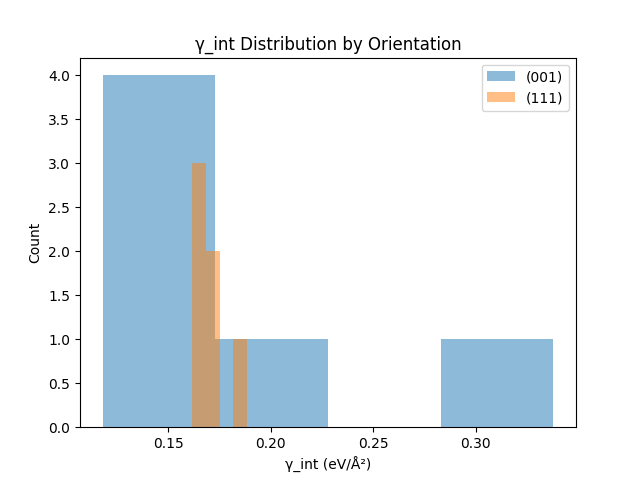
\includegraphics[width=0.7\textwidth]{gamma_distribution_colored.png}
\caption{
Distribution of interface formation energies ($\gamma_{\mathrm{int}}$) separated by orientation.
(001) interfaces exhibit a wider spread and tend toward somewhat lower values on average, while (111) interfaces are more narrowly distributed. With only 6 structures per orientation, these trends should be interpreted with caution.
}
\label{fig:gamma_distribution}
\end{figure}

Figure~\ref{fig:wad_vs_gamma} shows the relationship between $\gamma_{\mathrm{int}}$ and $W_{\mathrm{ad}}$. A weak correlation is observed, with lower $\gamma_{\mathrm{int}}$ generally corresponding to more negative $W_{\mathrm{ad}}$. However, the relationship is not strictly monotonic and exhibits noticeable scatter, particularly for (001) interfaces.

\begin{figure}[htbp]
\centering
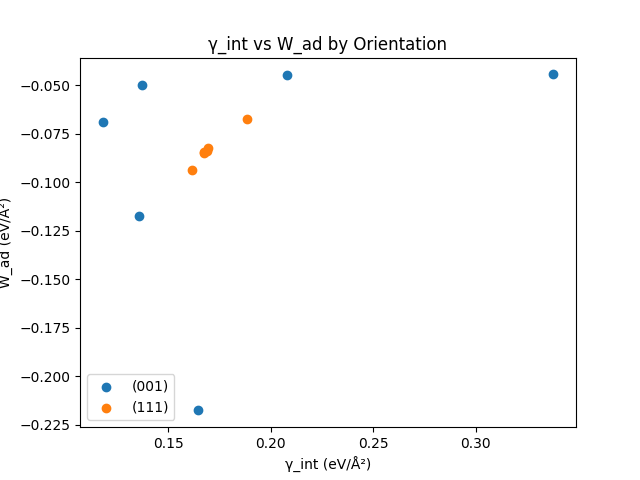
\includegraphics[width=0.7\textwidth]{wad_vs_gamma_colored.png}
\caption{
Relationship between interface formation energy ($\gamma_{\mathrm{int}}$) and work of adhesion ($W_{\mathrm{ad}}$), colored by interface orientation. A weak correlation is observed, with significant scatter. The small number of structures (12) limits the statistical significance of this trend.
}
\label{fig:wad_vs_gamma}
\end{figure}

\subsection{Interpretation}

The absence of a strict monotonic relationship between $\gamma_{\mathrm{int}}$ and $W_{\mathrm{ad}}$ reflects the fact that these quantities capture related but distinct physical properties. While $\gamma_{\mathrm{int}}$ characterizes the thermodynamic stability of the interface relative to bulk references, $W_{\mathrm{ad}}$ reflects the energetic cost of separating the interface into its constituent slabs. Both are sensitive to local bonding environments and atomic rearrangements, which can lead to deviations from a simple correspondence, particularly in systems with diverse terminations.

\subsection{Notable Configuration}

One (001) interface exhibits relatively strong adhesion ($W_{\mathrm{ad}} \approx -0.218$~eV/\AA$^2$), lying just outside the typical range reported by Iwasaki et al.~\cite{Iwasaki2022DFT_Li_LLZO_PSSB}. This likely reflects a particularly favorable local bonding configuration at this specific termination and highlights the importance of sampling diverse interface geometries.

\subsection{Summary}

The computed interface energetics are consistent with the prior DFT study of Iwasaki et al.\ in terms of energy scales and the dominant role of local atomic structure over crystallographic orientation. The present data are also consistent with the visual tendency in that work for (001) interfaces to cluster at lower formation energies, though the small dataset size prevents strong conclusions. These findings provide an additional layer of validation for the trained models, demonstrating their ability to reproduce physically meaningful interface behavior beyond standard energy and force error metrics.





\section{Molecular Dynamics of the Li(100)--LLZO(011) Interface}

%% CHANGED: removed broken Table~\ref{...}; replaced with prose reference
\subsection{Work of Adhesion for Li-Deficient LLZO Interfaces}
\label{sec:wad_vacancy}

To better represent the experimentally relevant situation in which tetragonal LLZO
contains a controlled concentration of lithium vacancies introduced by aliovalent
doping, the interface stacking procedure was repeated using vacancy-containing
LLZO slabs with the LLZO slab repeated $3\times$ and the Li slab repeated
$5\times$ along the stacking direction, compared to the single-repeat
building blocks used in Section~\ref{sec:interface_stacking}. The larger
Li slab ensures a sufficient reservoir of lithium metal at the interface,
avoiding artificial depletion effects that could arise if the metal layer
were too thin relative to the electrolyte slab.
Vacancies were introduced at a rate of two lithium sites removed per
192-atom LLZO formula unit, following
\begin{equation}
    n_{\mathrm{vac}} = \mathrm{round}\!\left(\frac{N_{\mathrm{LLZO}}}{192}\right) \times 2,
\end{equation}
where $N_{\mathrm{LLZO}}$ is the total number of atoms in the LLZO slab and the
rounding is to the nearest integer. Vacancy positions were selected using a fixed
random seed for reproducibility. The lithium metal slabs were kept defect-free
throughout.

The work of adhesion was computed (all energies with MACE-Iteration-1 model) following \eqnref{eq:Wad}, with $E_{\mathrm{slab,1}}$
taken as the energy of the isolated relaxed vacancy-containing LLZO slab and
$E_{\mathrm{slab,2}}$ as the energy of the isolated relaxed Li metal slab, divided
by the single interface area $A$. In all nine cases reported, the lithium atom count
satisfies $\Delta n_{\mathrm{Li}} = 0$, so no chemical potential correction is
required. Only Li(100) and Li(110) combinations that passed the $<$10\% in-plane
mismatch criterion are reported; Li(111) combinations were excluded on the same
grounds as in Chapter~3.

\begin{table}[htbp]
\centering
\caption{Work of adhesion $W_{\mathrm{ad}}$ for vacancy-containing Li--LLZO
interfaces, sorted by binding strength. LLZO slabs contain
$\mathrm{round}(N_{\mathrm{LLZO}}/192) \times 2$ lithium vacancies; Li slabs are
defect-free. All structures were relaxed with the Iteration~1 finetuned MACE
model prior to energy evaluation with the same model.}
\label{tab:wad_vacancy}
\begin{tabular}{clccc}
\hline
Rank & Interface & $A$ (\AA$^2$) & $W_{\mathrm{ad}}$ (eV/\AA$^2$) & $W_{\mathrm{ad}}$ (J/m$^2$) \\
\hline
1 & Li(110) / LLZO(011)-La & 241.96 & $-0.272$ & $-4.364$ \\
2 & Li(100) / LLZO(011)-La & 120.98 & $-0.183$ & $-2.932$ \\
3 & Li(100) / LLZO(110)-Zr & 118.62 & $-0.129$ & $-2.075$ \\
4 & Li(110) / LLZO(001)-Zr & 335.52 & $-0.116$ & $-1.860$ \\
5 & Li(110) / LLZO(110)-Li & 237.25 & $-0.088$ & $-1.408$ \\
6 & Li(110) / LLZO(010)-La & 335.52 & $-0.056$ & $-0.899$ \\
7 & Li(100) / LLZO(110)-Li & 118.62 & $-0.053$ & $-0.855$ \\
8 & Li(110) / LLZO(110)-Zr & 237.25 & $-0.043$ & $-0.686$ \\
9 & Li(100) / LLZO(010)-La & 167.76 & $-0.009$ & $-0.148$ \\
\hline
\end{tabular}
\end{table}

All nine values are negative, confirming favorable adhesion across all terminations
studied. The binding strengths span nearly two orders of magnitude, from
$-0.009$~eV/\AA$^2$ for Li(100)/LLZO(010)-La to $-0.272$~eV/\AA$^2$ for
Li(110)/LLZO(011)-La, reinforcing the conclusion of Section~\ref{sec:energetics}
that surface termination is the dominant determinant of interfacial binding strength.
La-terminated LLZO(011) surfaces consistently produce the strongest adhesion
regardless of Li facet, while La-terminated LLZO(010) and the Li-terminated
LLZO(110) surfaces exhibit the weakest binding. These values are somewhat larger
in magnitude than the stoichiometric interface results of Section~\ref{sec:energetics}
and the DFT range reported by Iwasaki et al.~\cite{Iwasaki2022DFT_Li_LLZO_PSSB},
which is physically reasonable: the presence of lithium vacancies in the LLZO
surface creates undercoordinated sites that bond more strongly to the incoming
lithium metal.

The Li(100)/LLZO(011)-La interface (Rank~2, $W_{\mathrm{ad}} = -0.183$~eV/\AA$^2$)
was selected for the detailed MD analysis presented below. This choice was motivated
by two practical considerations: first, this configuration was already part of the
active learning MD pool across both Iterations~0 and~1, meaning a fully relaxed
starting geometry consistent with the training data was directly available; second,
its interface area ($A = 120.98$~\AA$^2$) is approximately half that of the
highest-ranking structure (Li(110)/LLZO(011)-La, $A = 241.96$~\AA$^2$), making
200~ps NVT trajectories significantly less expensive while still probing a strongly
adhesive interface.

\subsection{Scope and Limitations}

It is important to emphasize that the present MD analysis is \textit{qualitative} in nature. While the finetuned model demonstrates strong accuracy in energy predictions, its force predictions can exhibit larger deviations in out-of-distribution (OOD) regimes, as discussed in Section~\ref{sec:ood}.

Since MD simulations are directly driven by forces, this introduces limitations in the quantitative reliability of long-time dynamical behaviour. Therefore, the results presented here should be interpreted as physically indicative trends rather than precise quantitative predictions of interfacial kinetics or transport.

%% CHANGED: added explicit validation context paragraph connecting to PI concern
%% about whether the MLIP has been sufficiently validated.
\paragraph{Multi-level validation context --}
The reliability of the present MD analysis rests on a hierarchy of validation tests that collectively support the physical interpretations drawn below. At the first level, energy and force RMSE on held-out validation structures within the training distribution are below 5~meV/atom and $\sim$55~meV/\AA\ respectively (Sections~\ref{sec:results_it0} and~\ref{sec:results_it1}). At the second level, cohesive energy and force predictions on eight OOD interface geometries derived from a structurally distinct LLZO source show consistent improvement over the universal baseline (Section~\ref{sec:ood}). At the third level, interface formation energies and works of adhesion are in agreement with the range reported by the prior DFT study of Iwasaki et al.~\cite{Iwasaki2022DFT_Li_LLZO_PSSB} (Section~\ref{sec:energetics}). Together, these three levels of validation provide confidence that the model captures the relevant chemistry of the Li--LLZO interface. We note, however, that a more stringent structural validation --- comparing pair
distribution functions between MLIP-MD trajectories and DFT single-point labels
on MD-sampled structures --- has not been performed in this work and constitutes
an important direction for future validation before drawing quantitative conclusions
about transport properties.


\subsection{Simulation Details}

MD simulations were performed using the Iteration 0 finetuned MACE model under the following conditions:

\begin{itemize}
    \item Temperature: 298 K
    \item Total simulation time: 200 ps
    \item Time step: 0.5 fs
    \item Ensemble: NVT (Langevin thermostat)
    \item Boundary conditions: periodic in-plane ($x$, $y$), non-periodic along $z$
\end{itemize}

A spatially restricted active region was employed to ensure stability of the slab geometry while allowing interfacial dynamics. Approximately 40\% of the LLZO slab near the interface and 25\% of the lithium slab were allowed to evolve dynamically, with a minimum active thickness of 6~\AA. The remaining atoms were held fixed.

\subsection{Time Evolution and Equilibration}

The interface undergoes an initial relaxation phase followed by a steady-state regime. Based on time-series analysis, the system stabilizes within $\sim$20 ps and reaches a steady regime by $\sim$25--30 ps.

\begin{figure}[htbp]
\centering
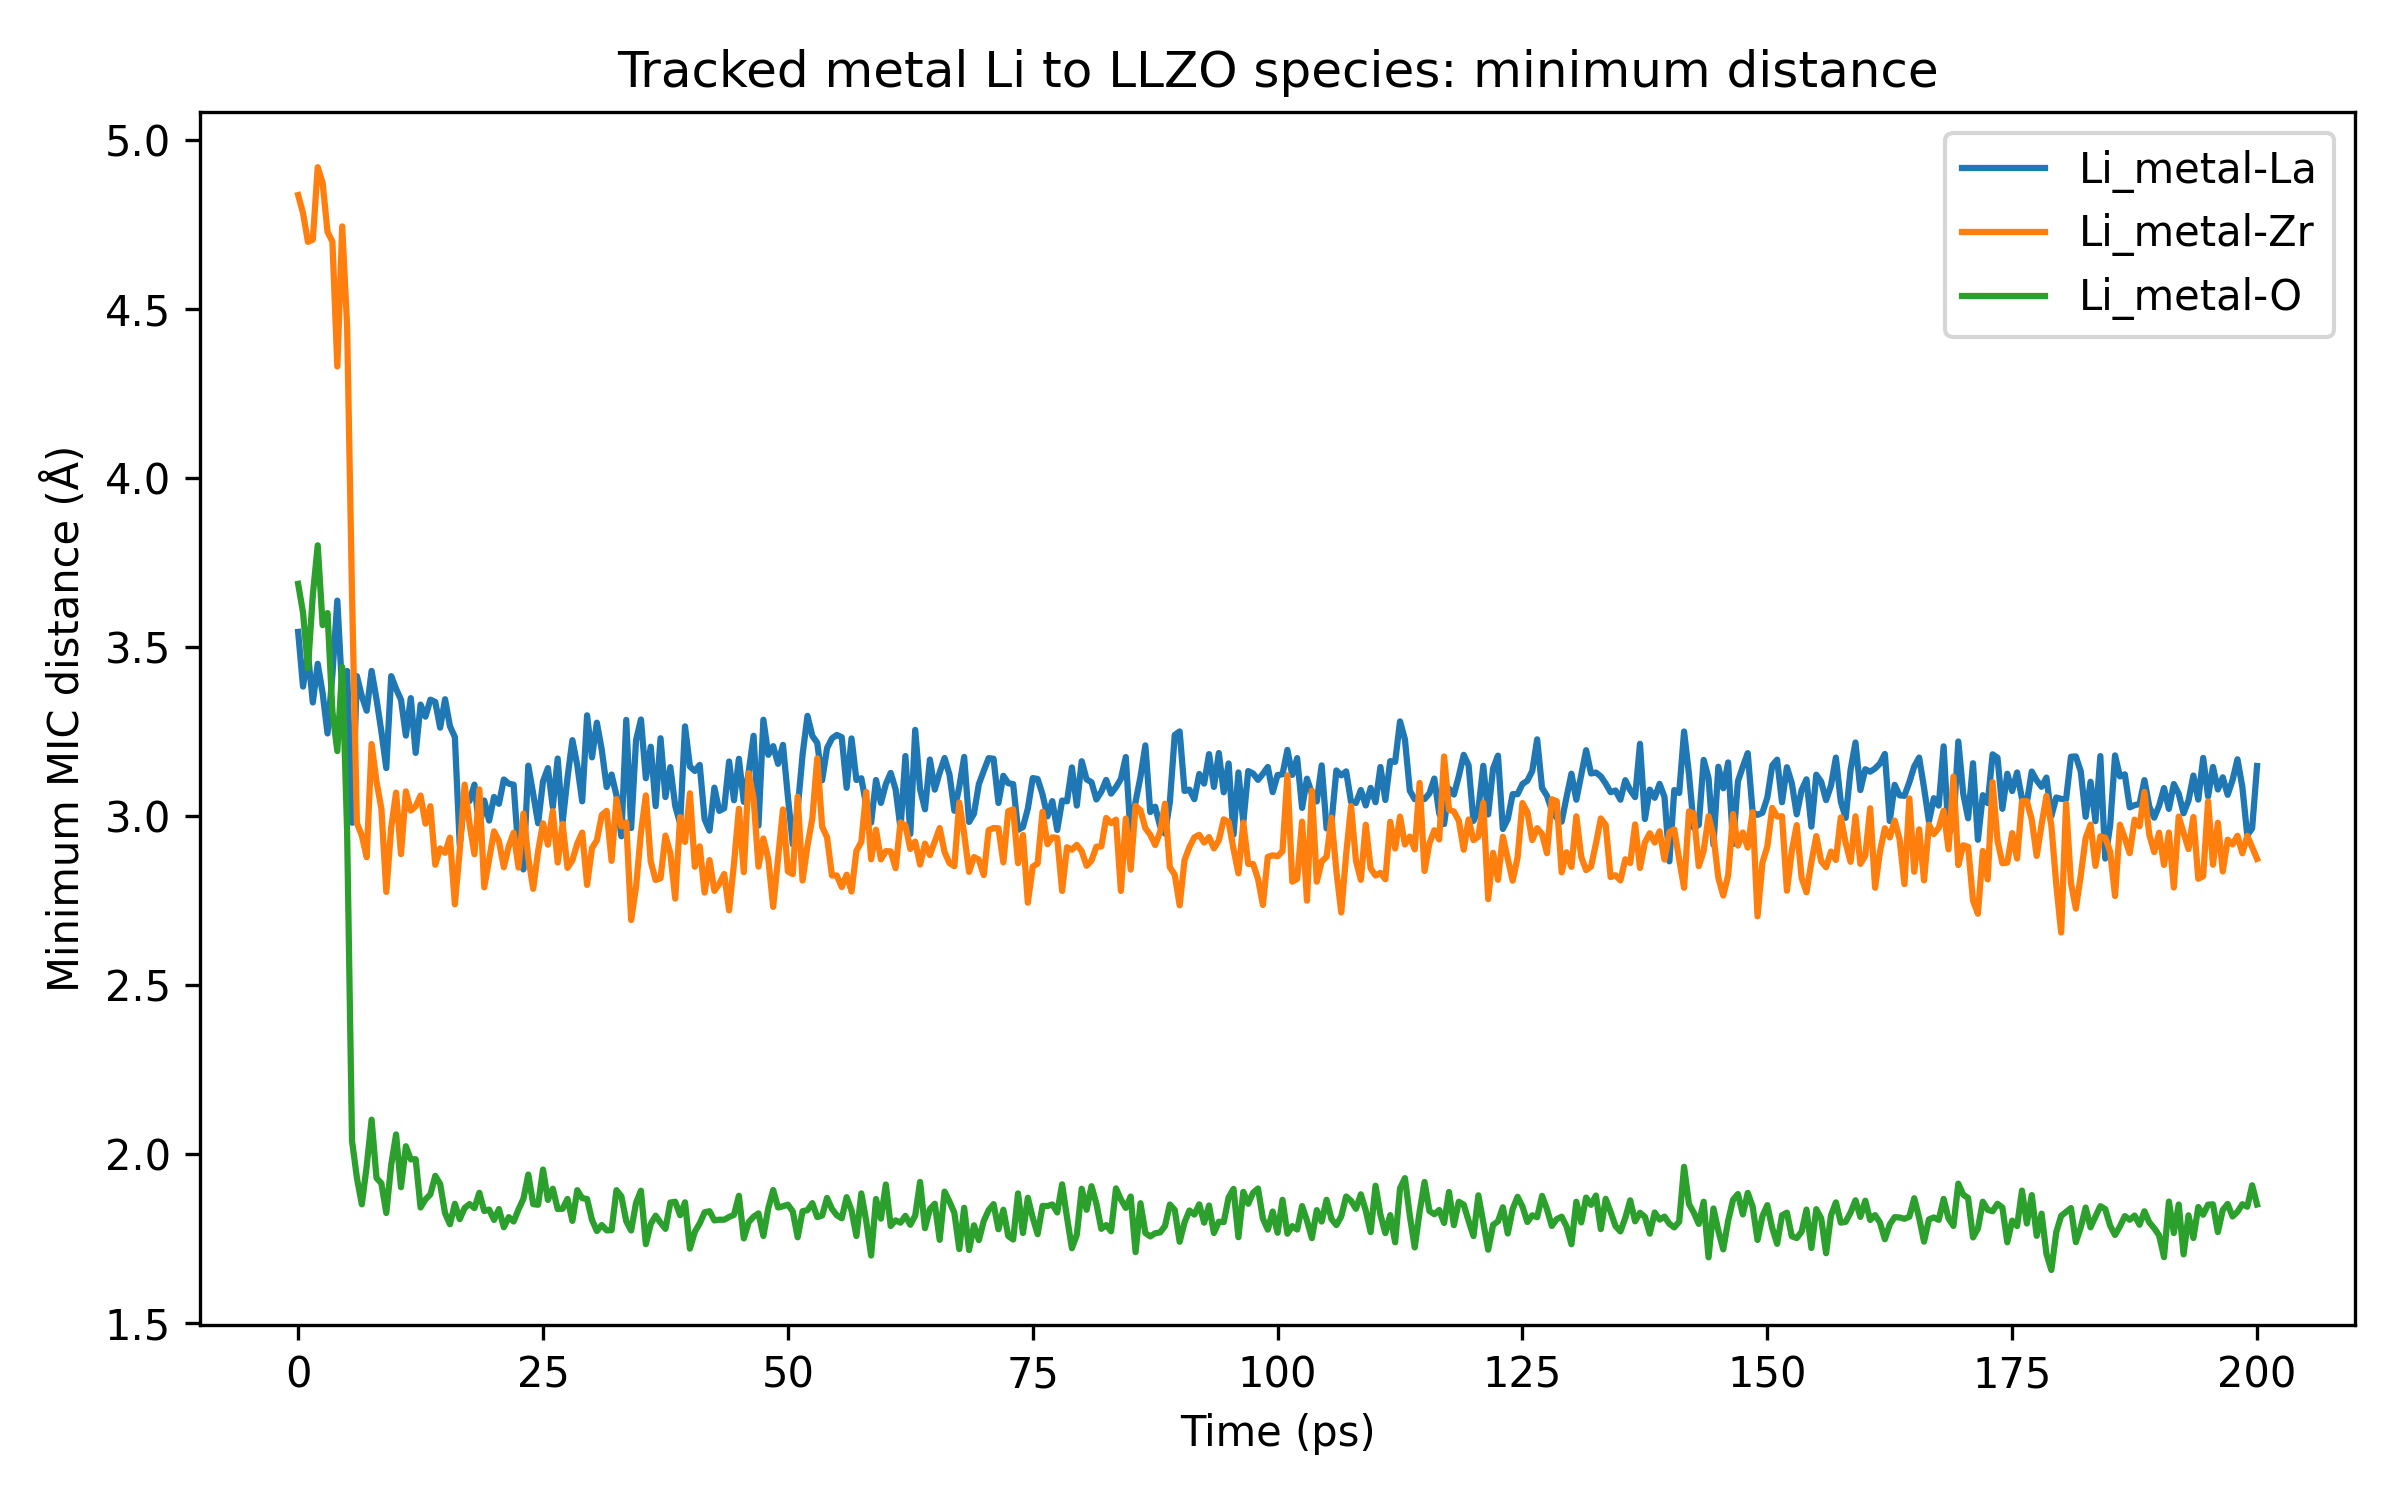
\includegraphics[width=0.7\textwidth]{min_interfacial_distances.png}
\caption{
Evolution of minimum interfacial distances. The Li--O distance decreases during the initial relaxation phase and stabilizes around 1.8--1.9~\AA, indicating formation of a stable contact layer.
}
\end{figure}

\begin{itemize}
    \item \textbf{Minimum interfacial distances:} Rapid relaxation within the first $\sim$10--15 ps followed by stabilization.
    \item \textbf{Penetration depth:} Reaches a shallow steady range ($\sim$0.8--1.3~\AA) and fluctuates thermally thereafter.
    \item \textbf{Framework RMSD:} Increases initially and then plateaus, indicating equilibration.
    \item \textbf{Structural metrics:} Oxide thickness and slab separation remain stable throughout.
\end{itemize}

\subsection{Interface Stability Analysis}

\paragraph{Absence of Li penetration --}

\begin{figure}[htbp]
\centering
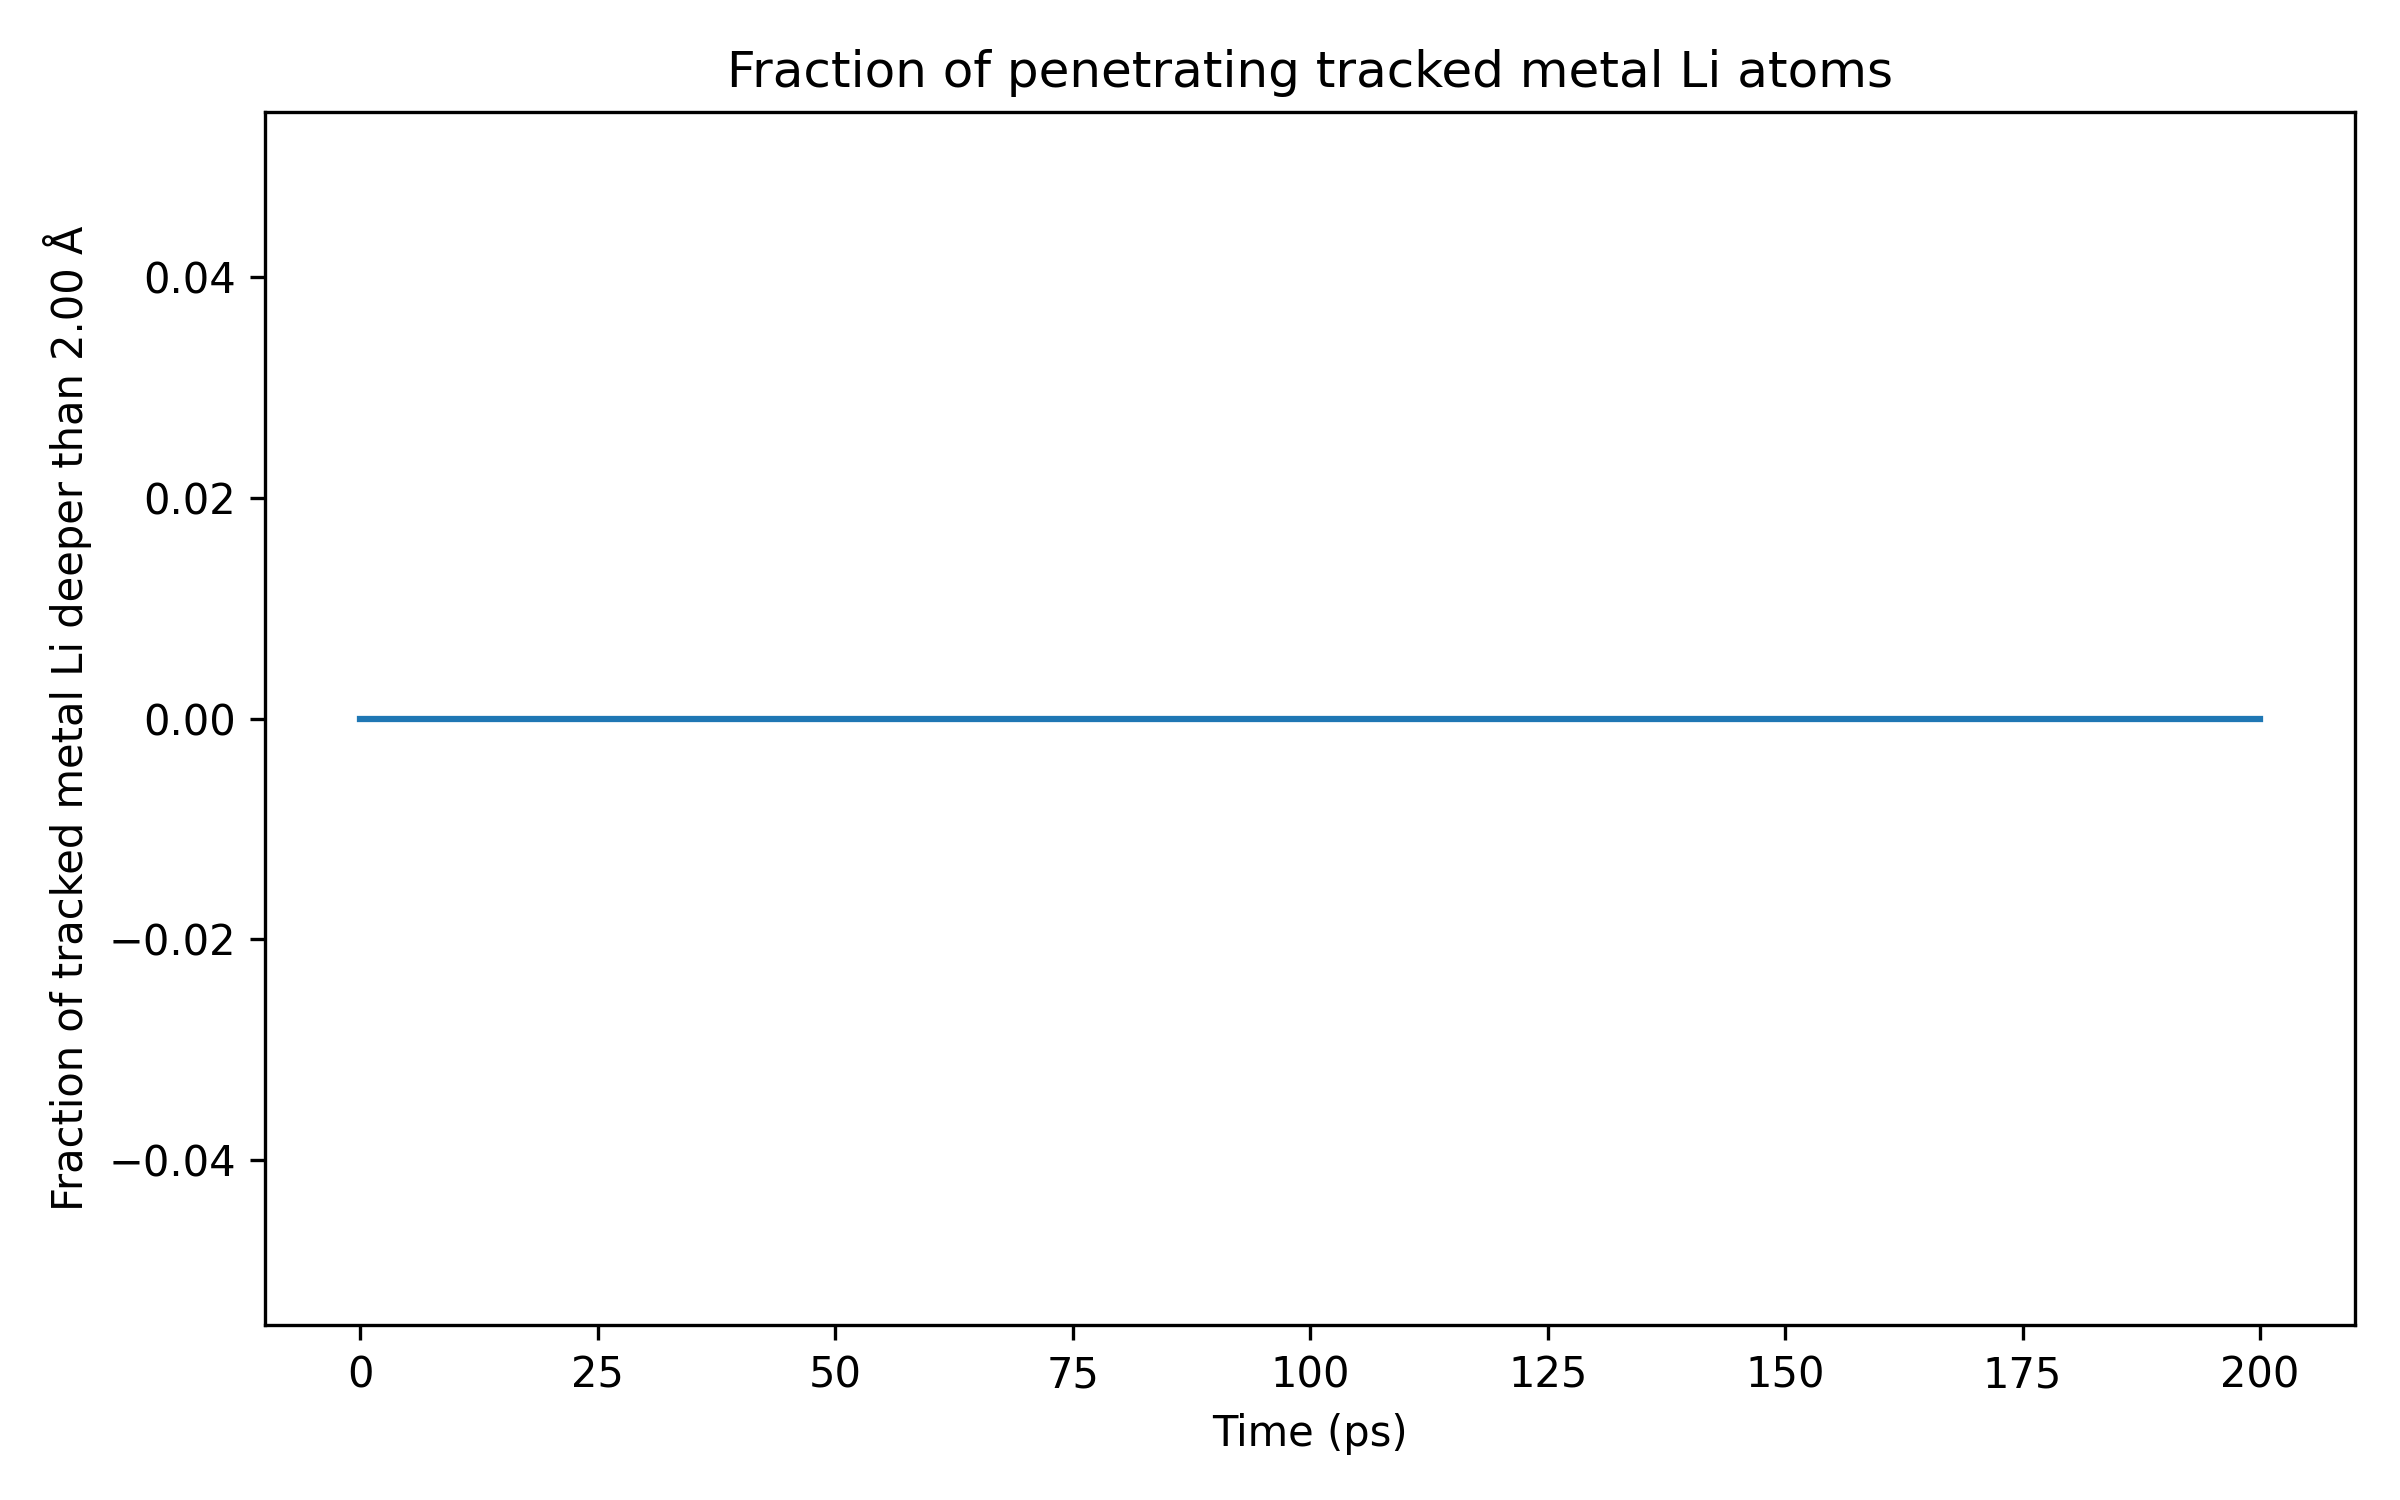
\includegraphics[width=0.7\textwidth]{li_penetration_fraction.png}
\caption{
Fraction of lithium atoms penetrating more than 2~\AA\ into LLZO. The value remains zero throughout the simulation, indicating absence of insertion events.
}
\end{figure}

No lithium atoms penetrate beyond 2~\AA\ into the LLZO slab at any point during the simulation. The maximum observed penetration depth ($\sim$1.4~\AA) corresponds to surface contact rather than insertion.

\paragraph{Penetration dynamics --}

\begin{figure}[htbp]
\centering
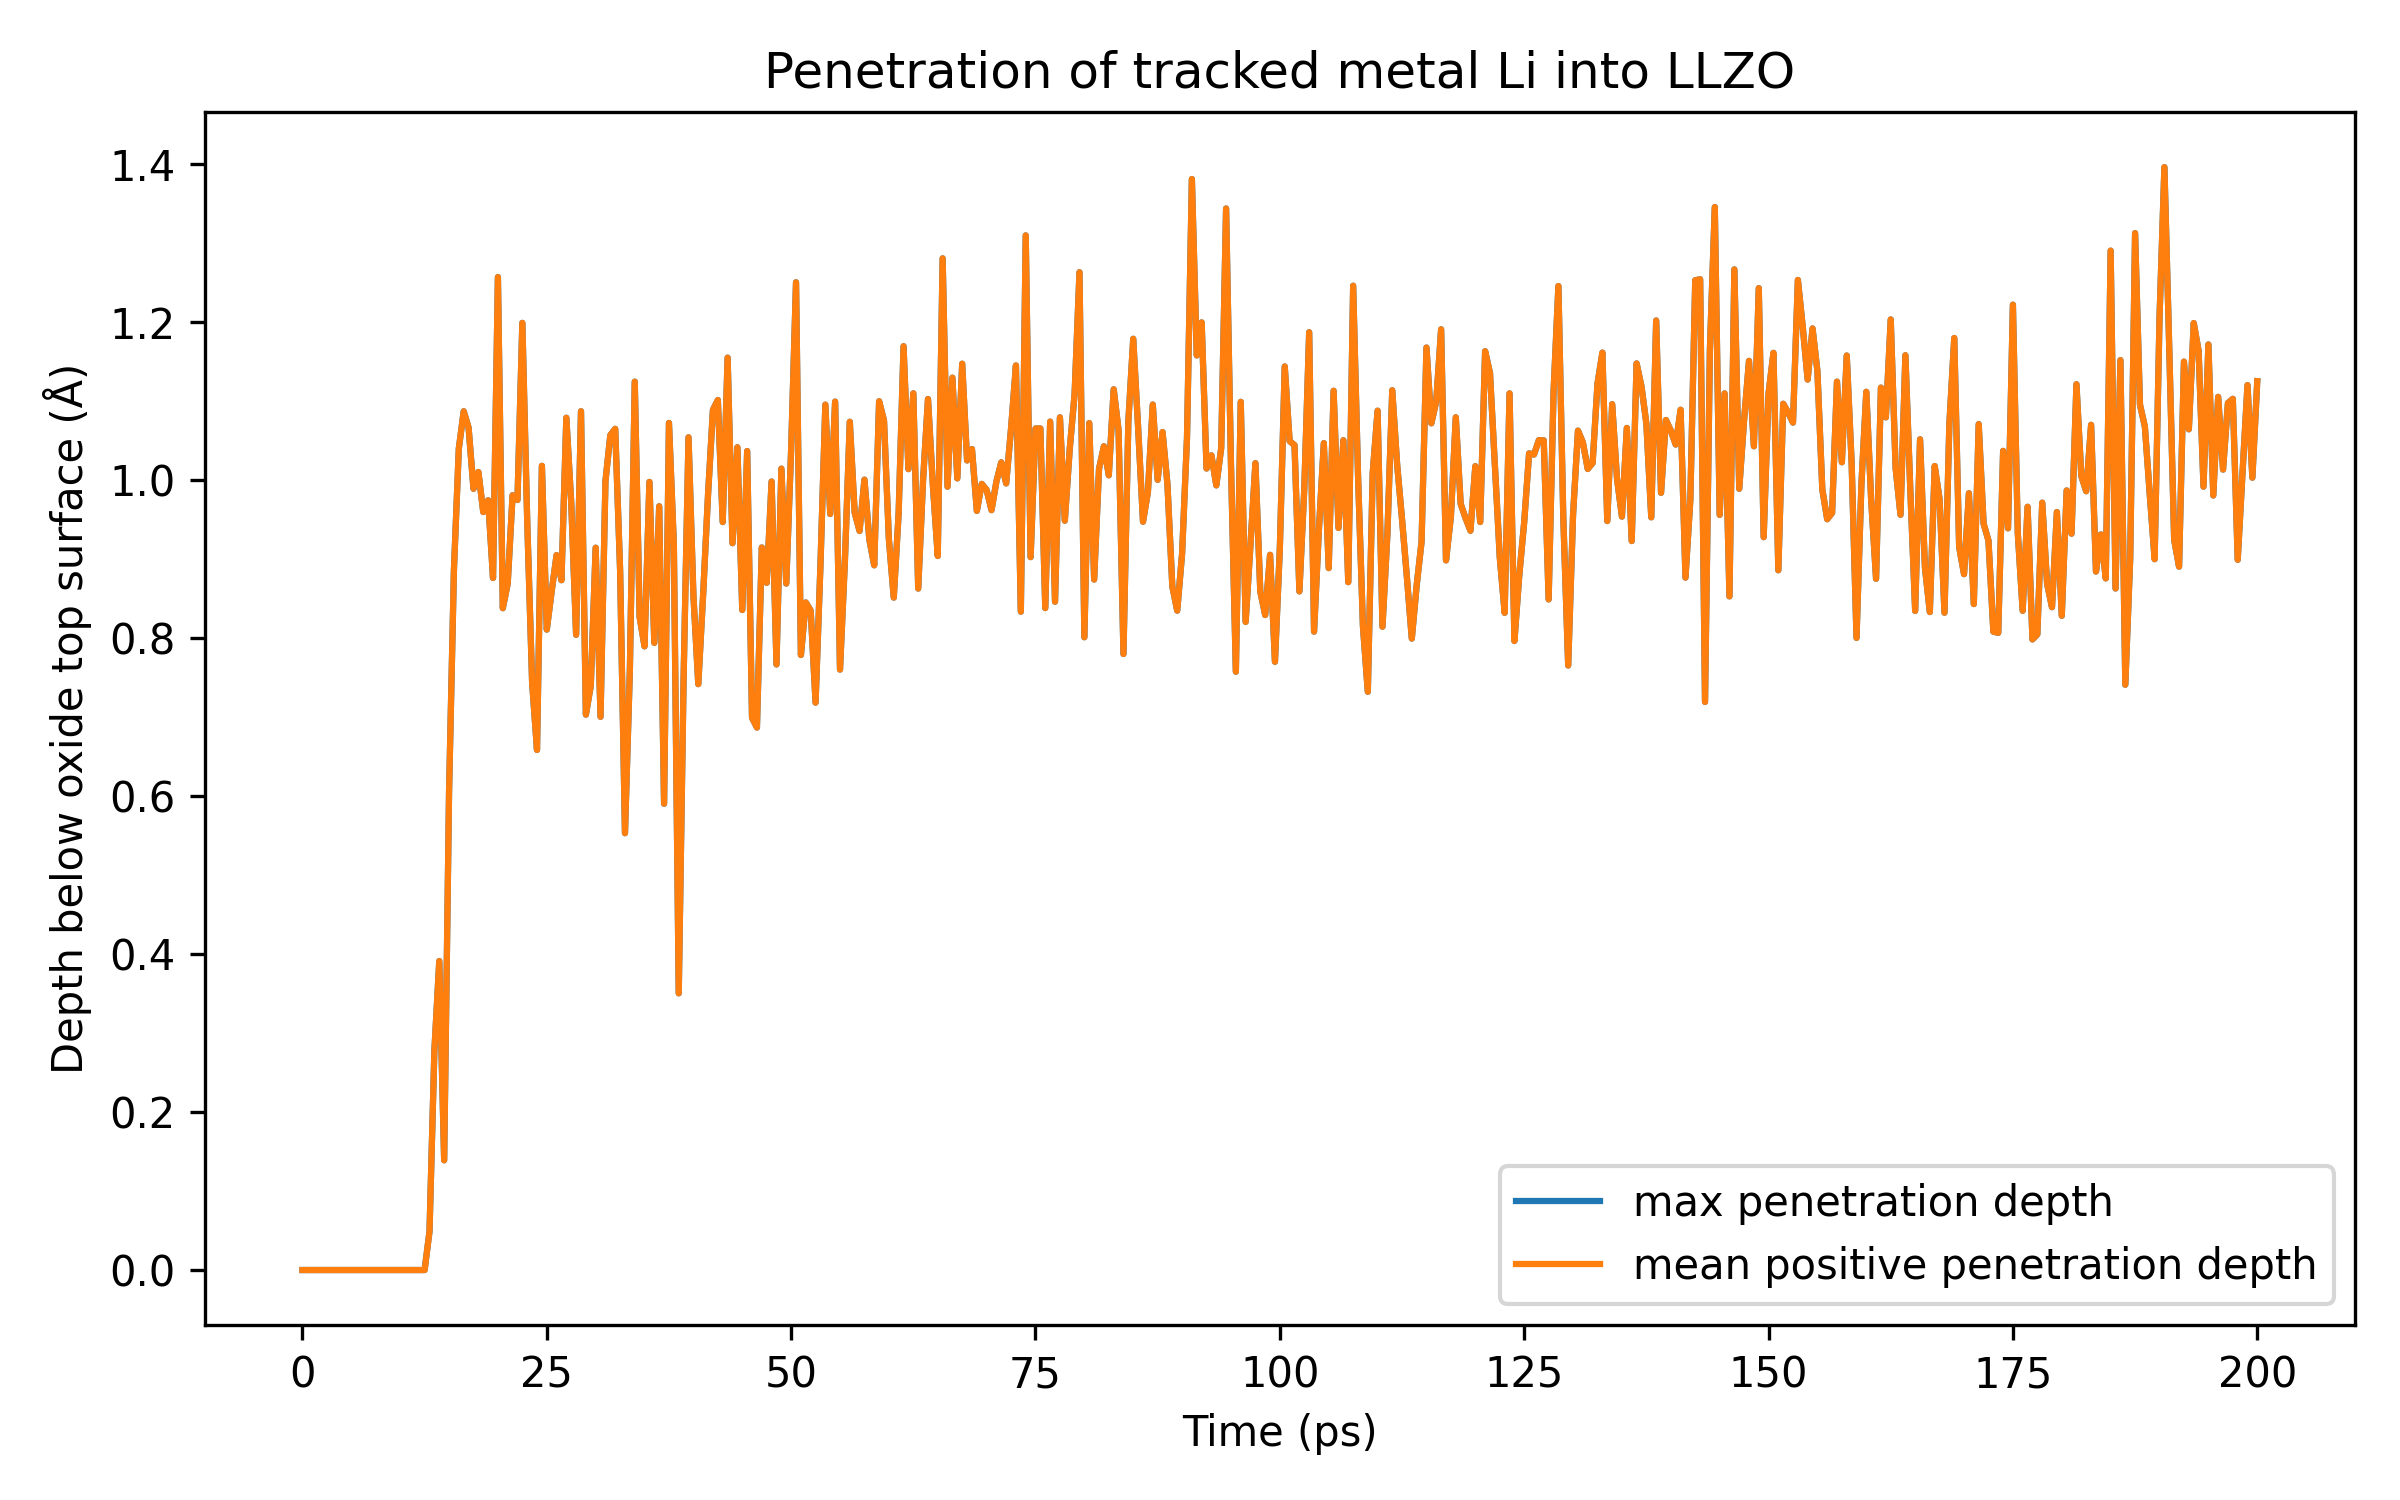
\includegraphics[width=0.7\textwidth]{li_penetration_depth.png}
\caption{
Time evolution of lithium penetration depth. After initial relaxation, penetration remains shallow and fluctuates within a narrow range.
}
\end{figure}

Penetration depth stabilizes early and does not exhibit any monotonic increase or deep insertion events.

\paragraph{Preservation of LLZO framework --}

\begin{figure}[htbp]
\centering
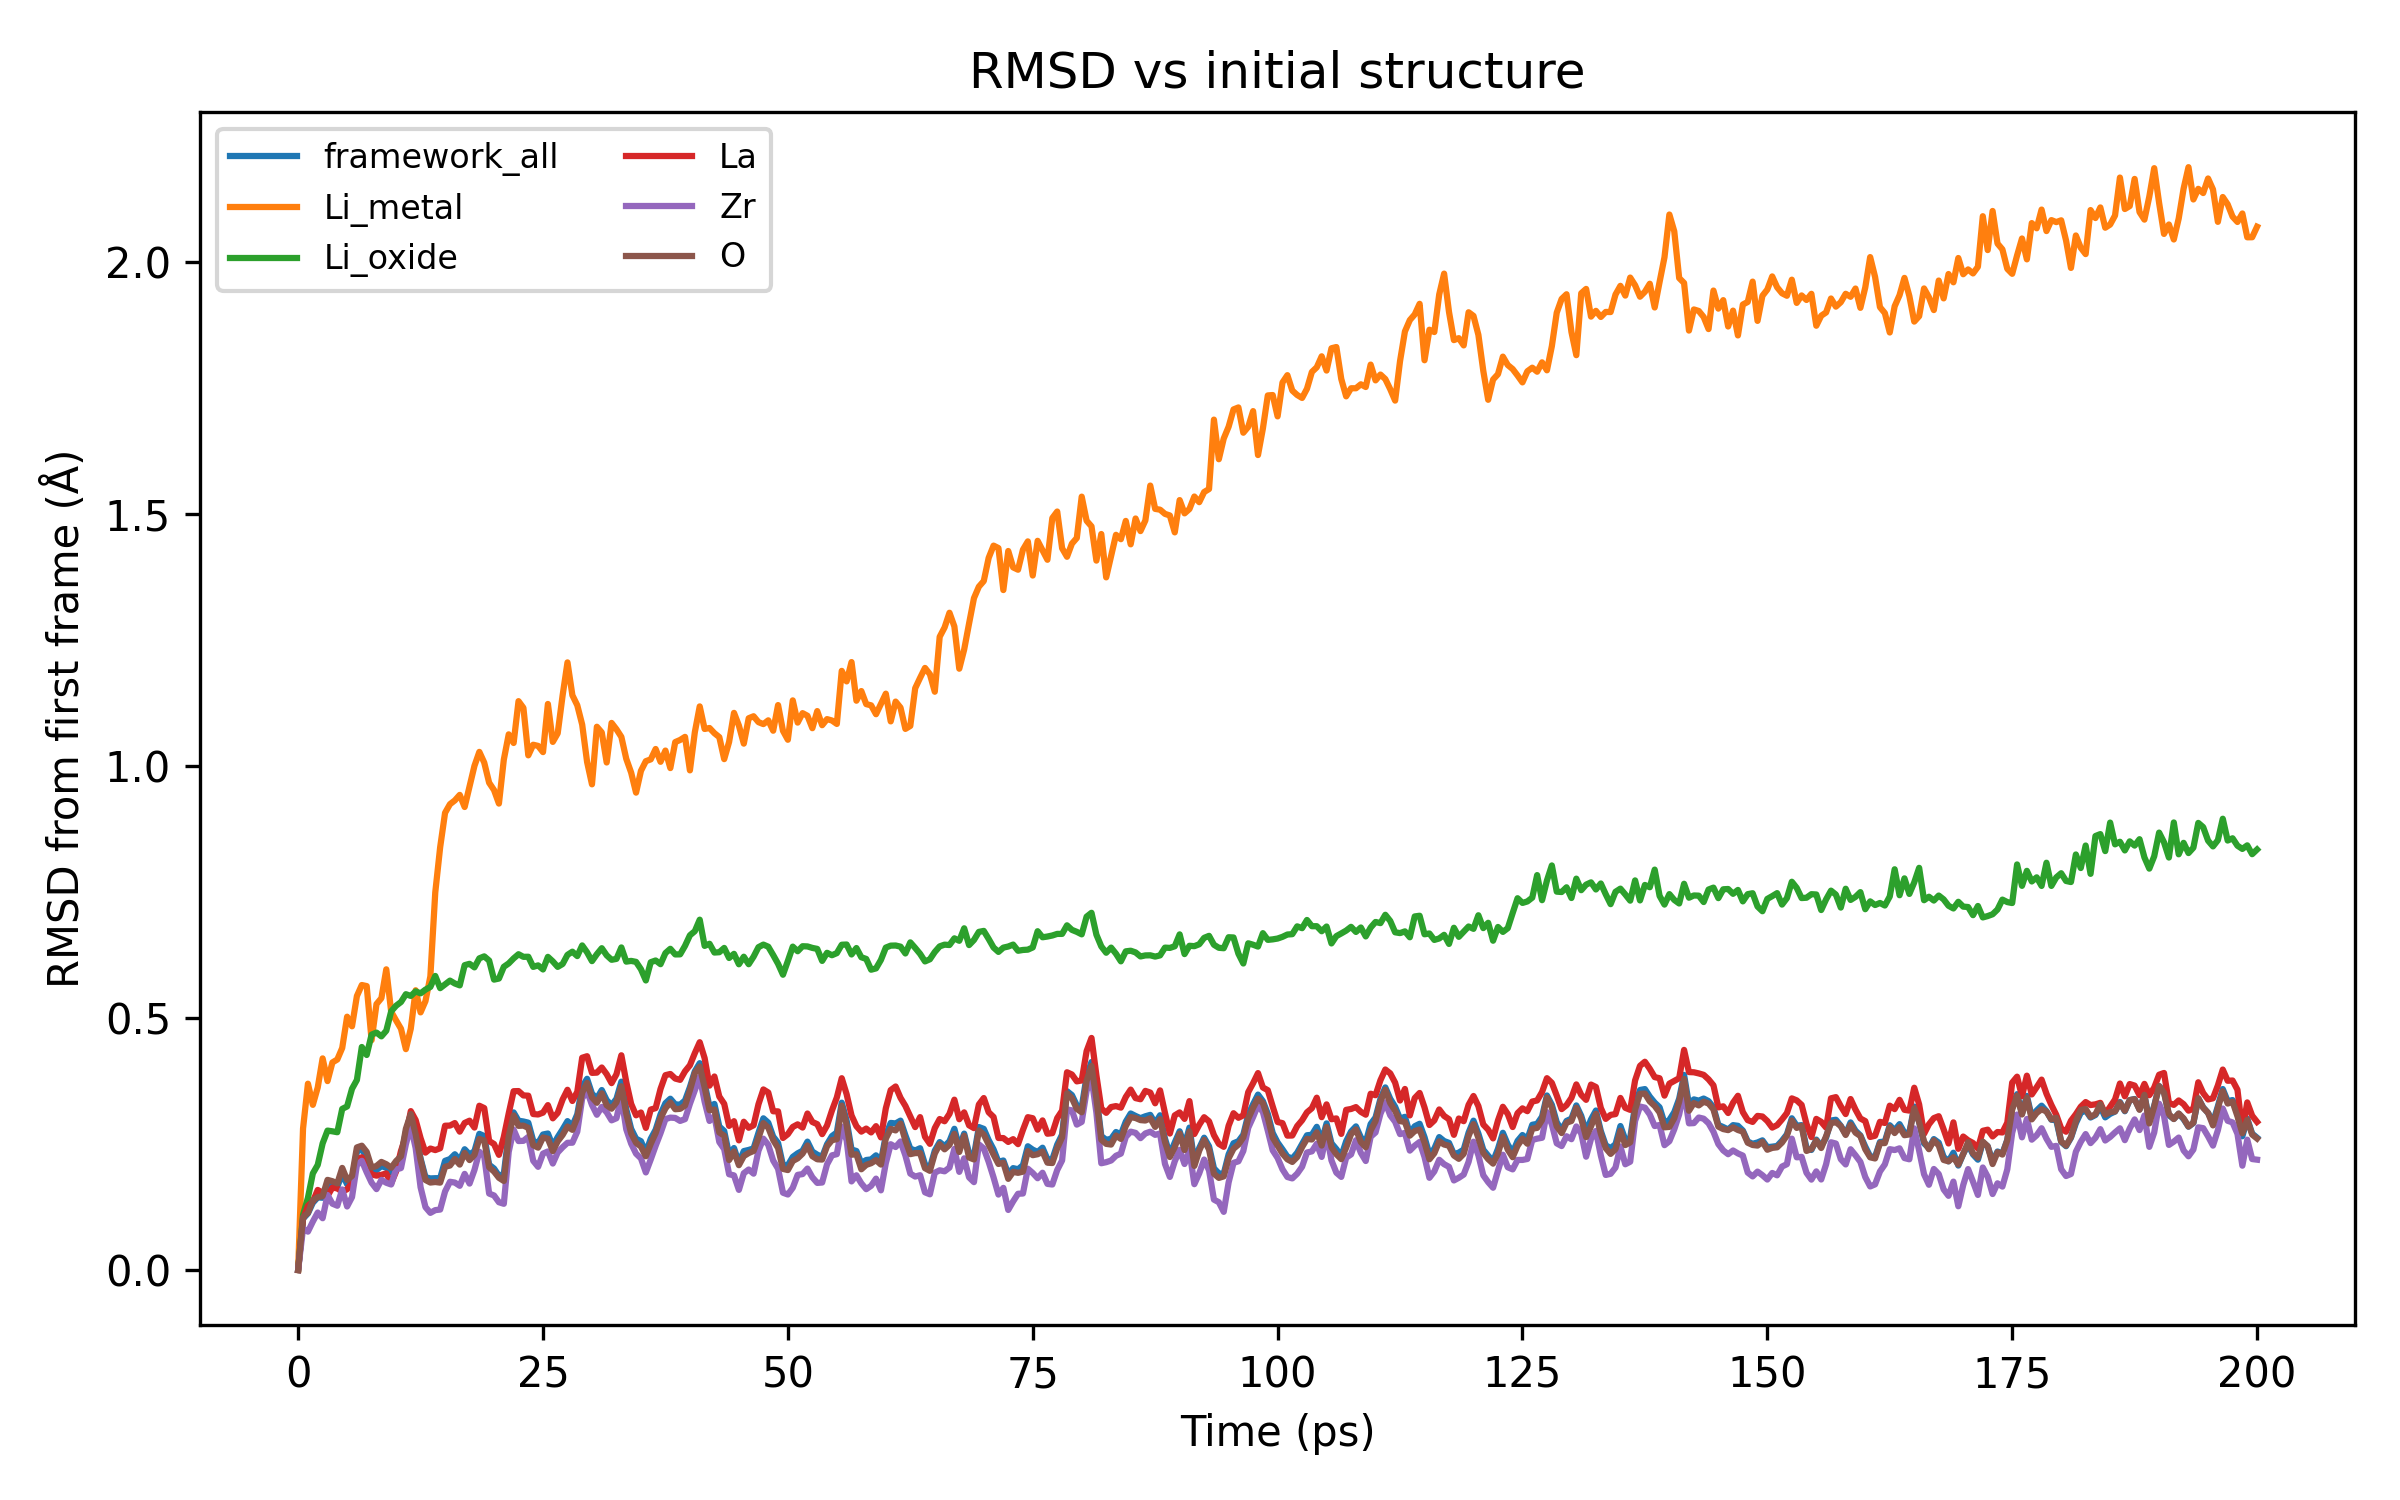
\includegraphics[width=0.7\textwidth]{rmsd_species.png}
\caption{
RMSD of atomic species. The LLZO framework shows low and stable RMSD, indicating structural integrity throughout the simulation.
}
\end{figure}

The LLZO lattice remains structurally intact, with framework RMSD stabilizing at $\sim$0.28~\AA.

\paragraph{Atomic mobility --}

\begin{figure}[htbp]
\centering
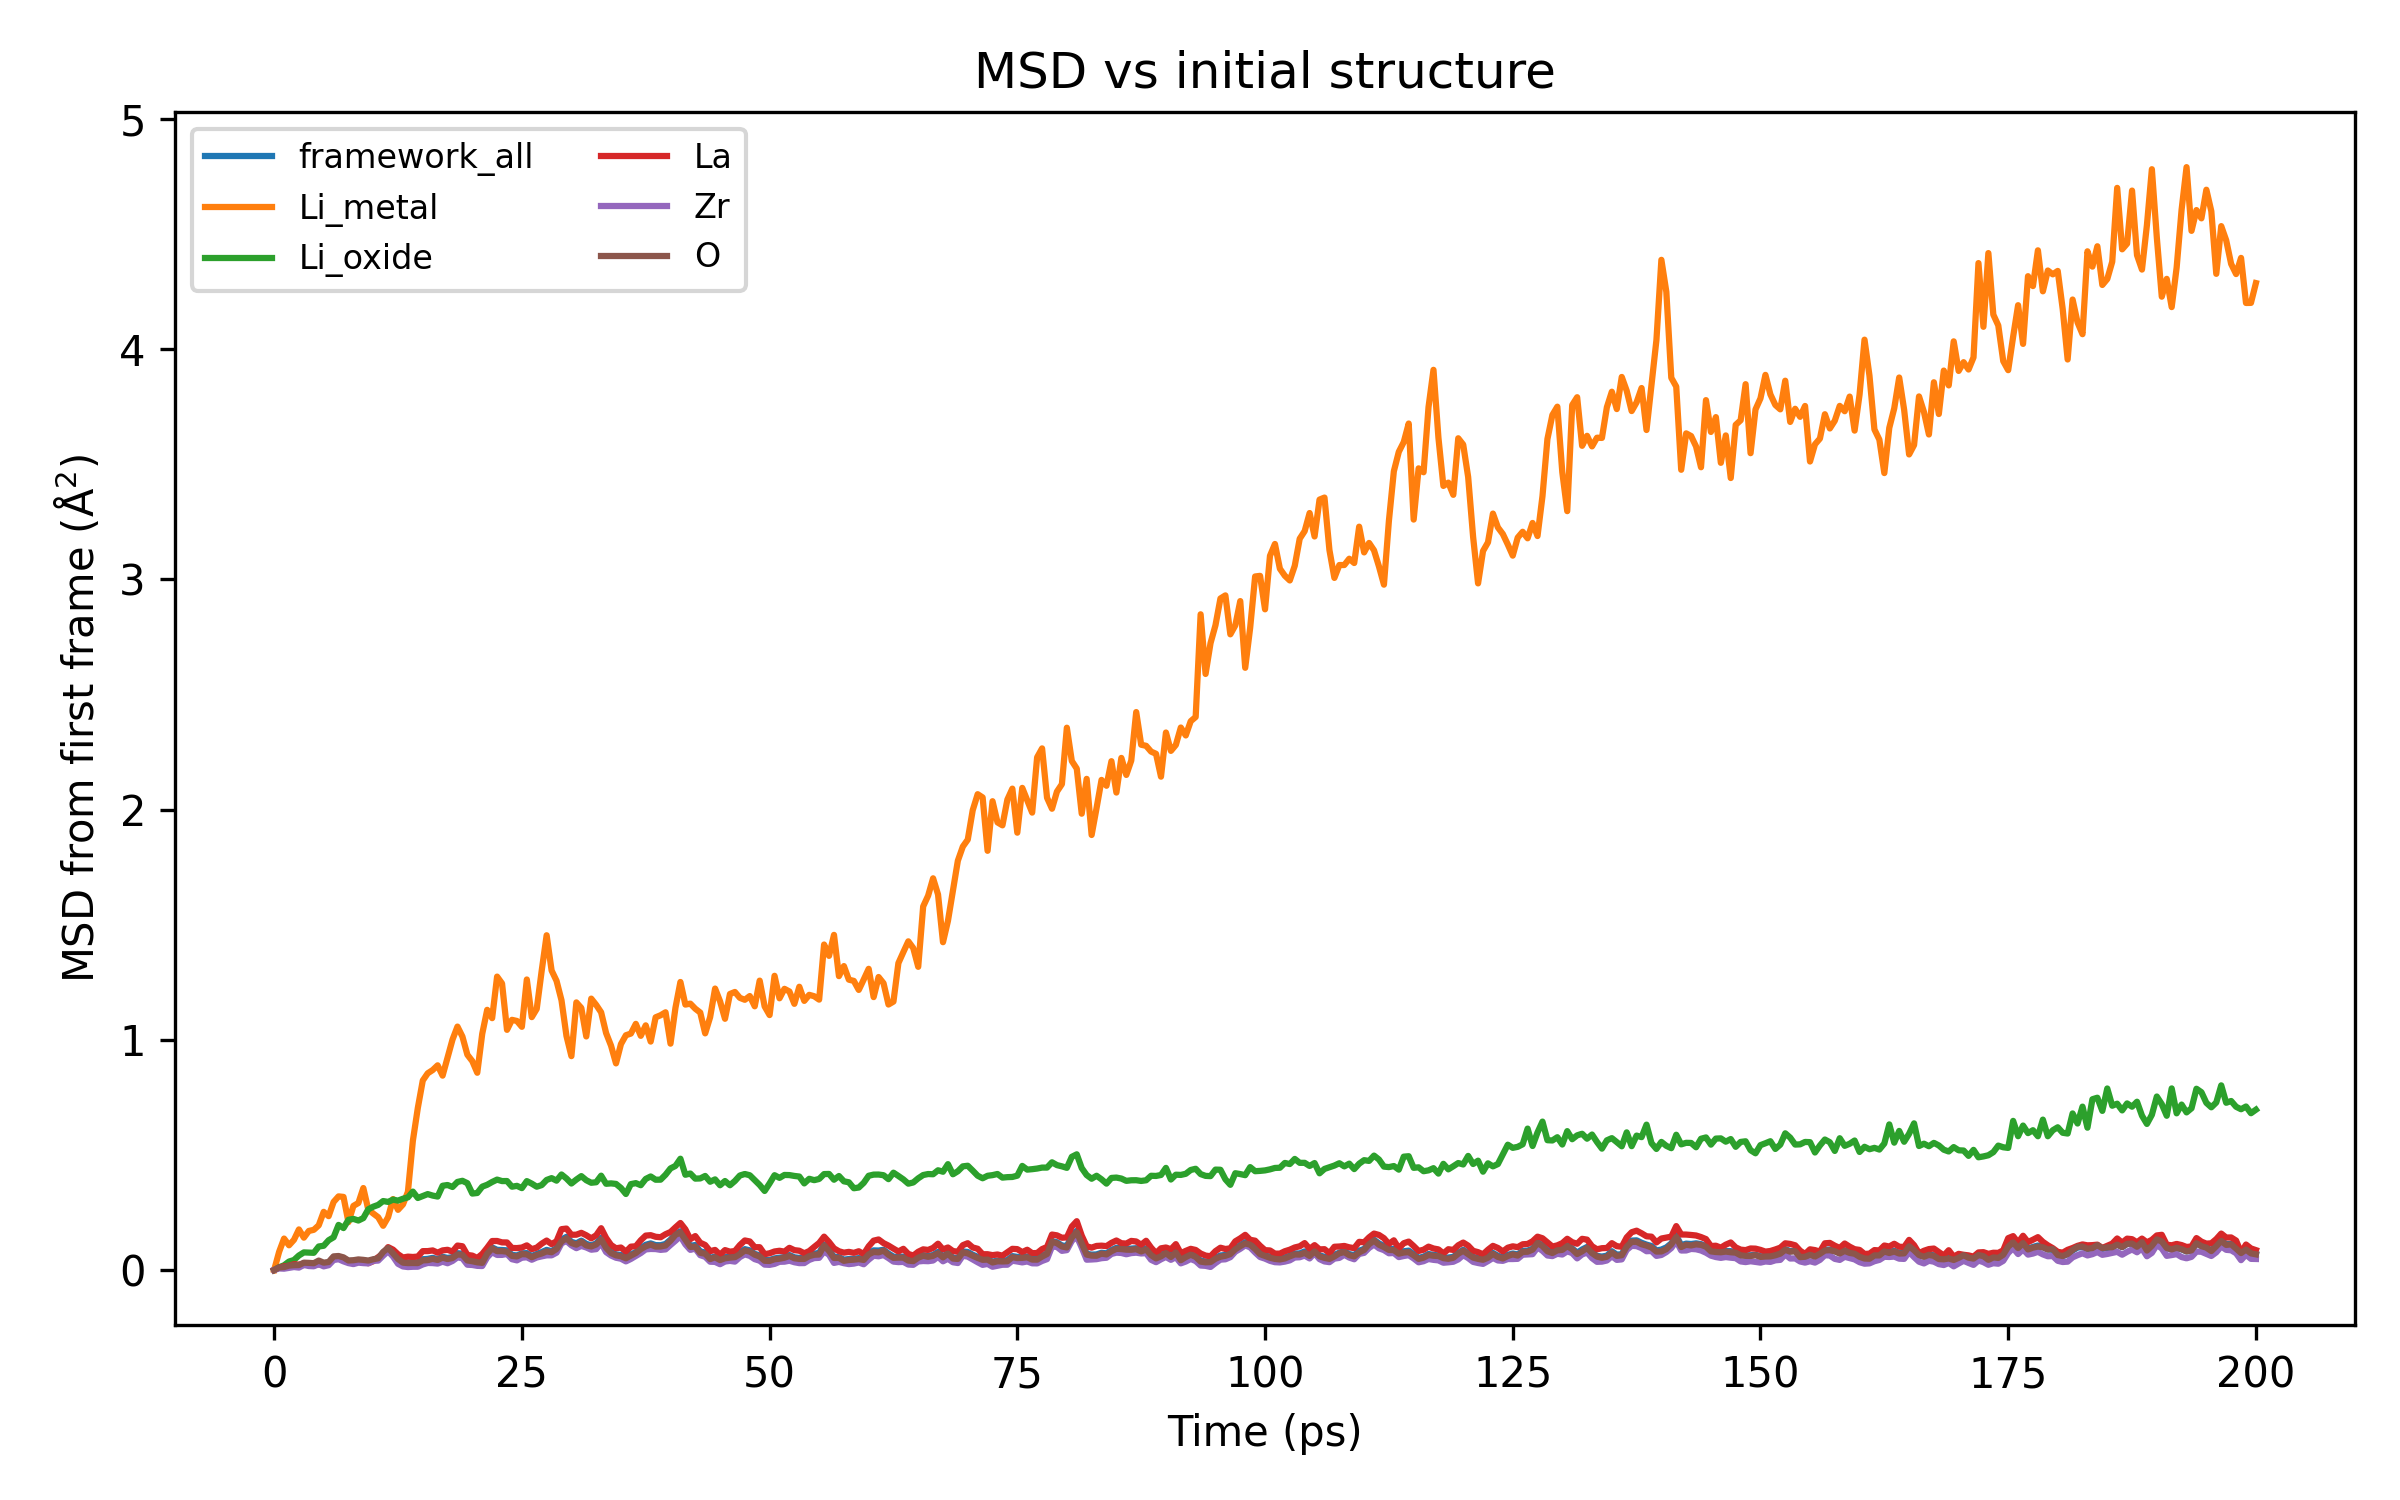
\includegraphics[width=0.7\textwidth]{msd_species.png}
\caption{
Mean-squared displacement (MSD) of different species. Lithium metal shows the highest mobility, while framework atoms remain nearly stationary.
}
\end{figure}

A physically consistent mobility hierarchy is observed:
\[
\text{Li}_{\text{metal}} > \text{Li}_{\text{oxide}} > \text{framework}
\]

\paragraph{Interface morphology --}

\begin{figure}[htbp]
\centering
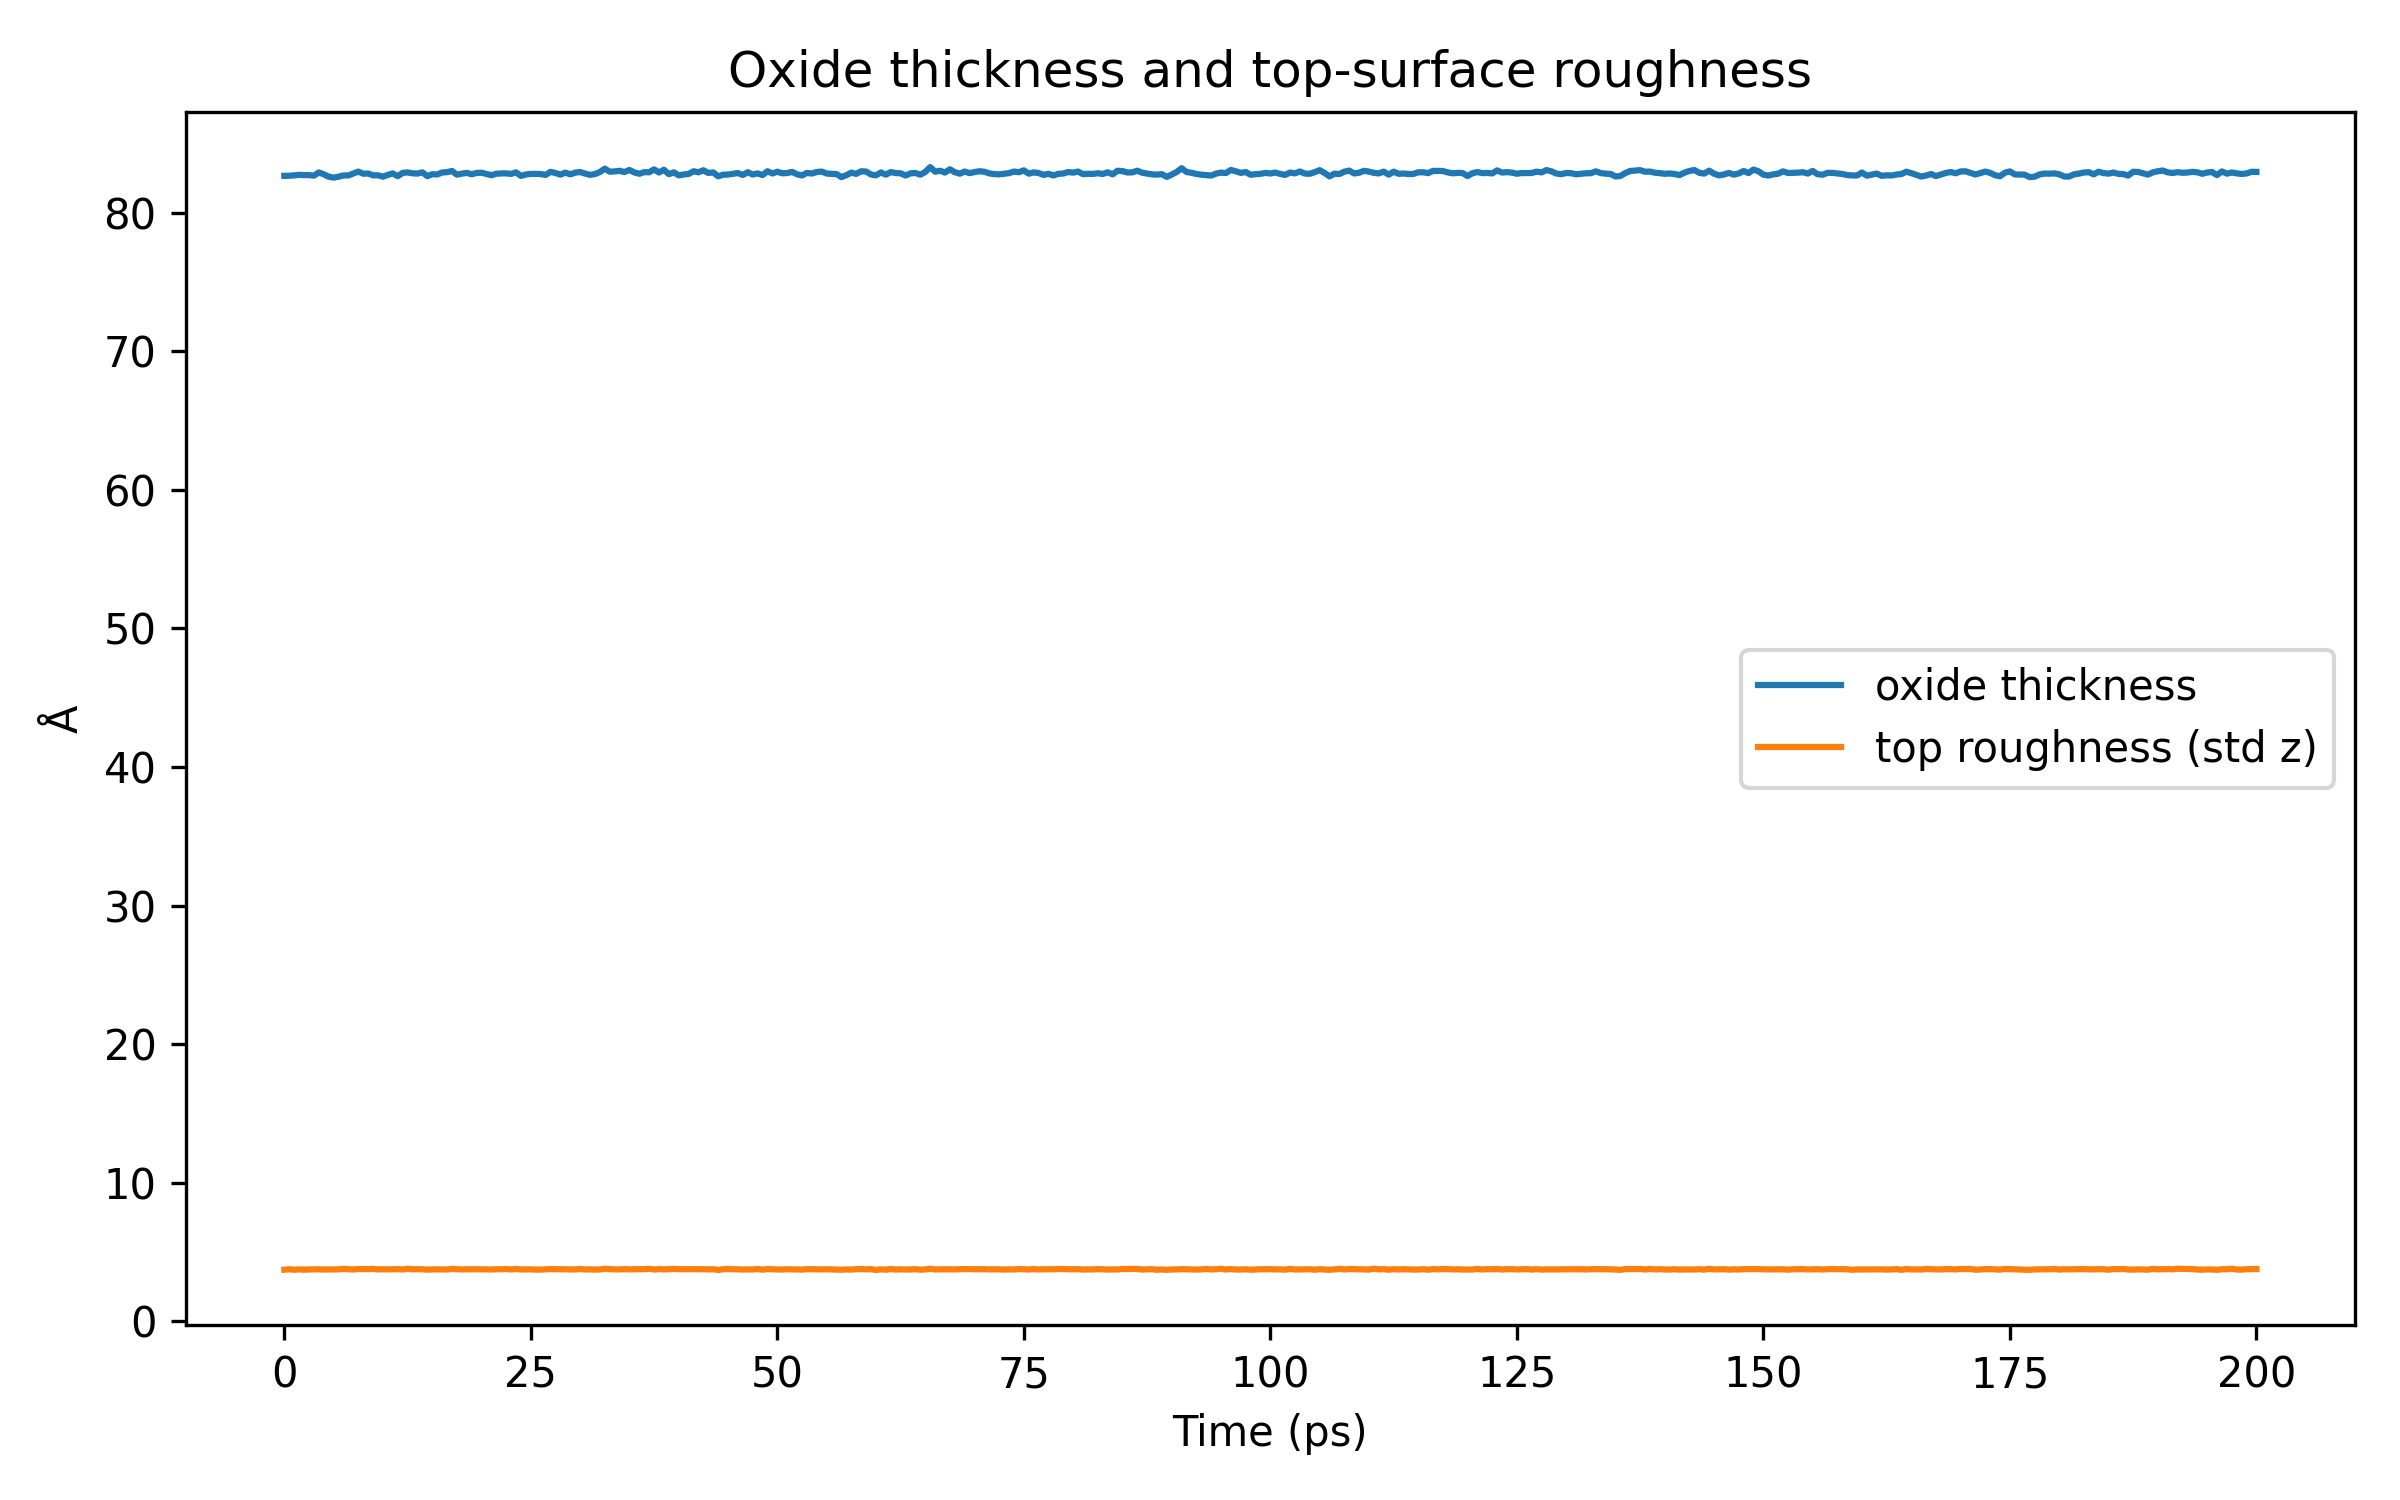
\includegraphics[width=0.7\textwidth]{oxide_thickness_roughness.png}
\caption{
Oxide thickness and surface roughness as a function of time. Both quantities remain stable, indicating absence of structural degradation.
}
\end{figure}

\begin{figure}[htbp]
\centering
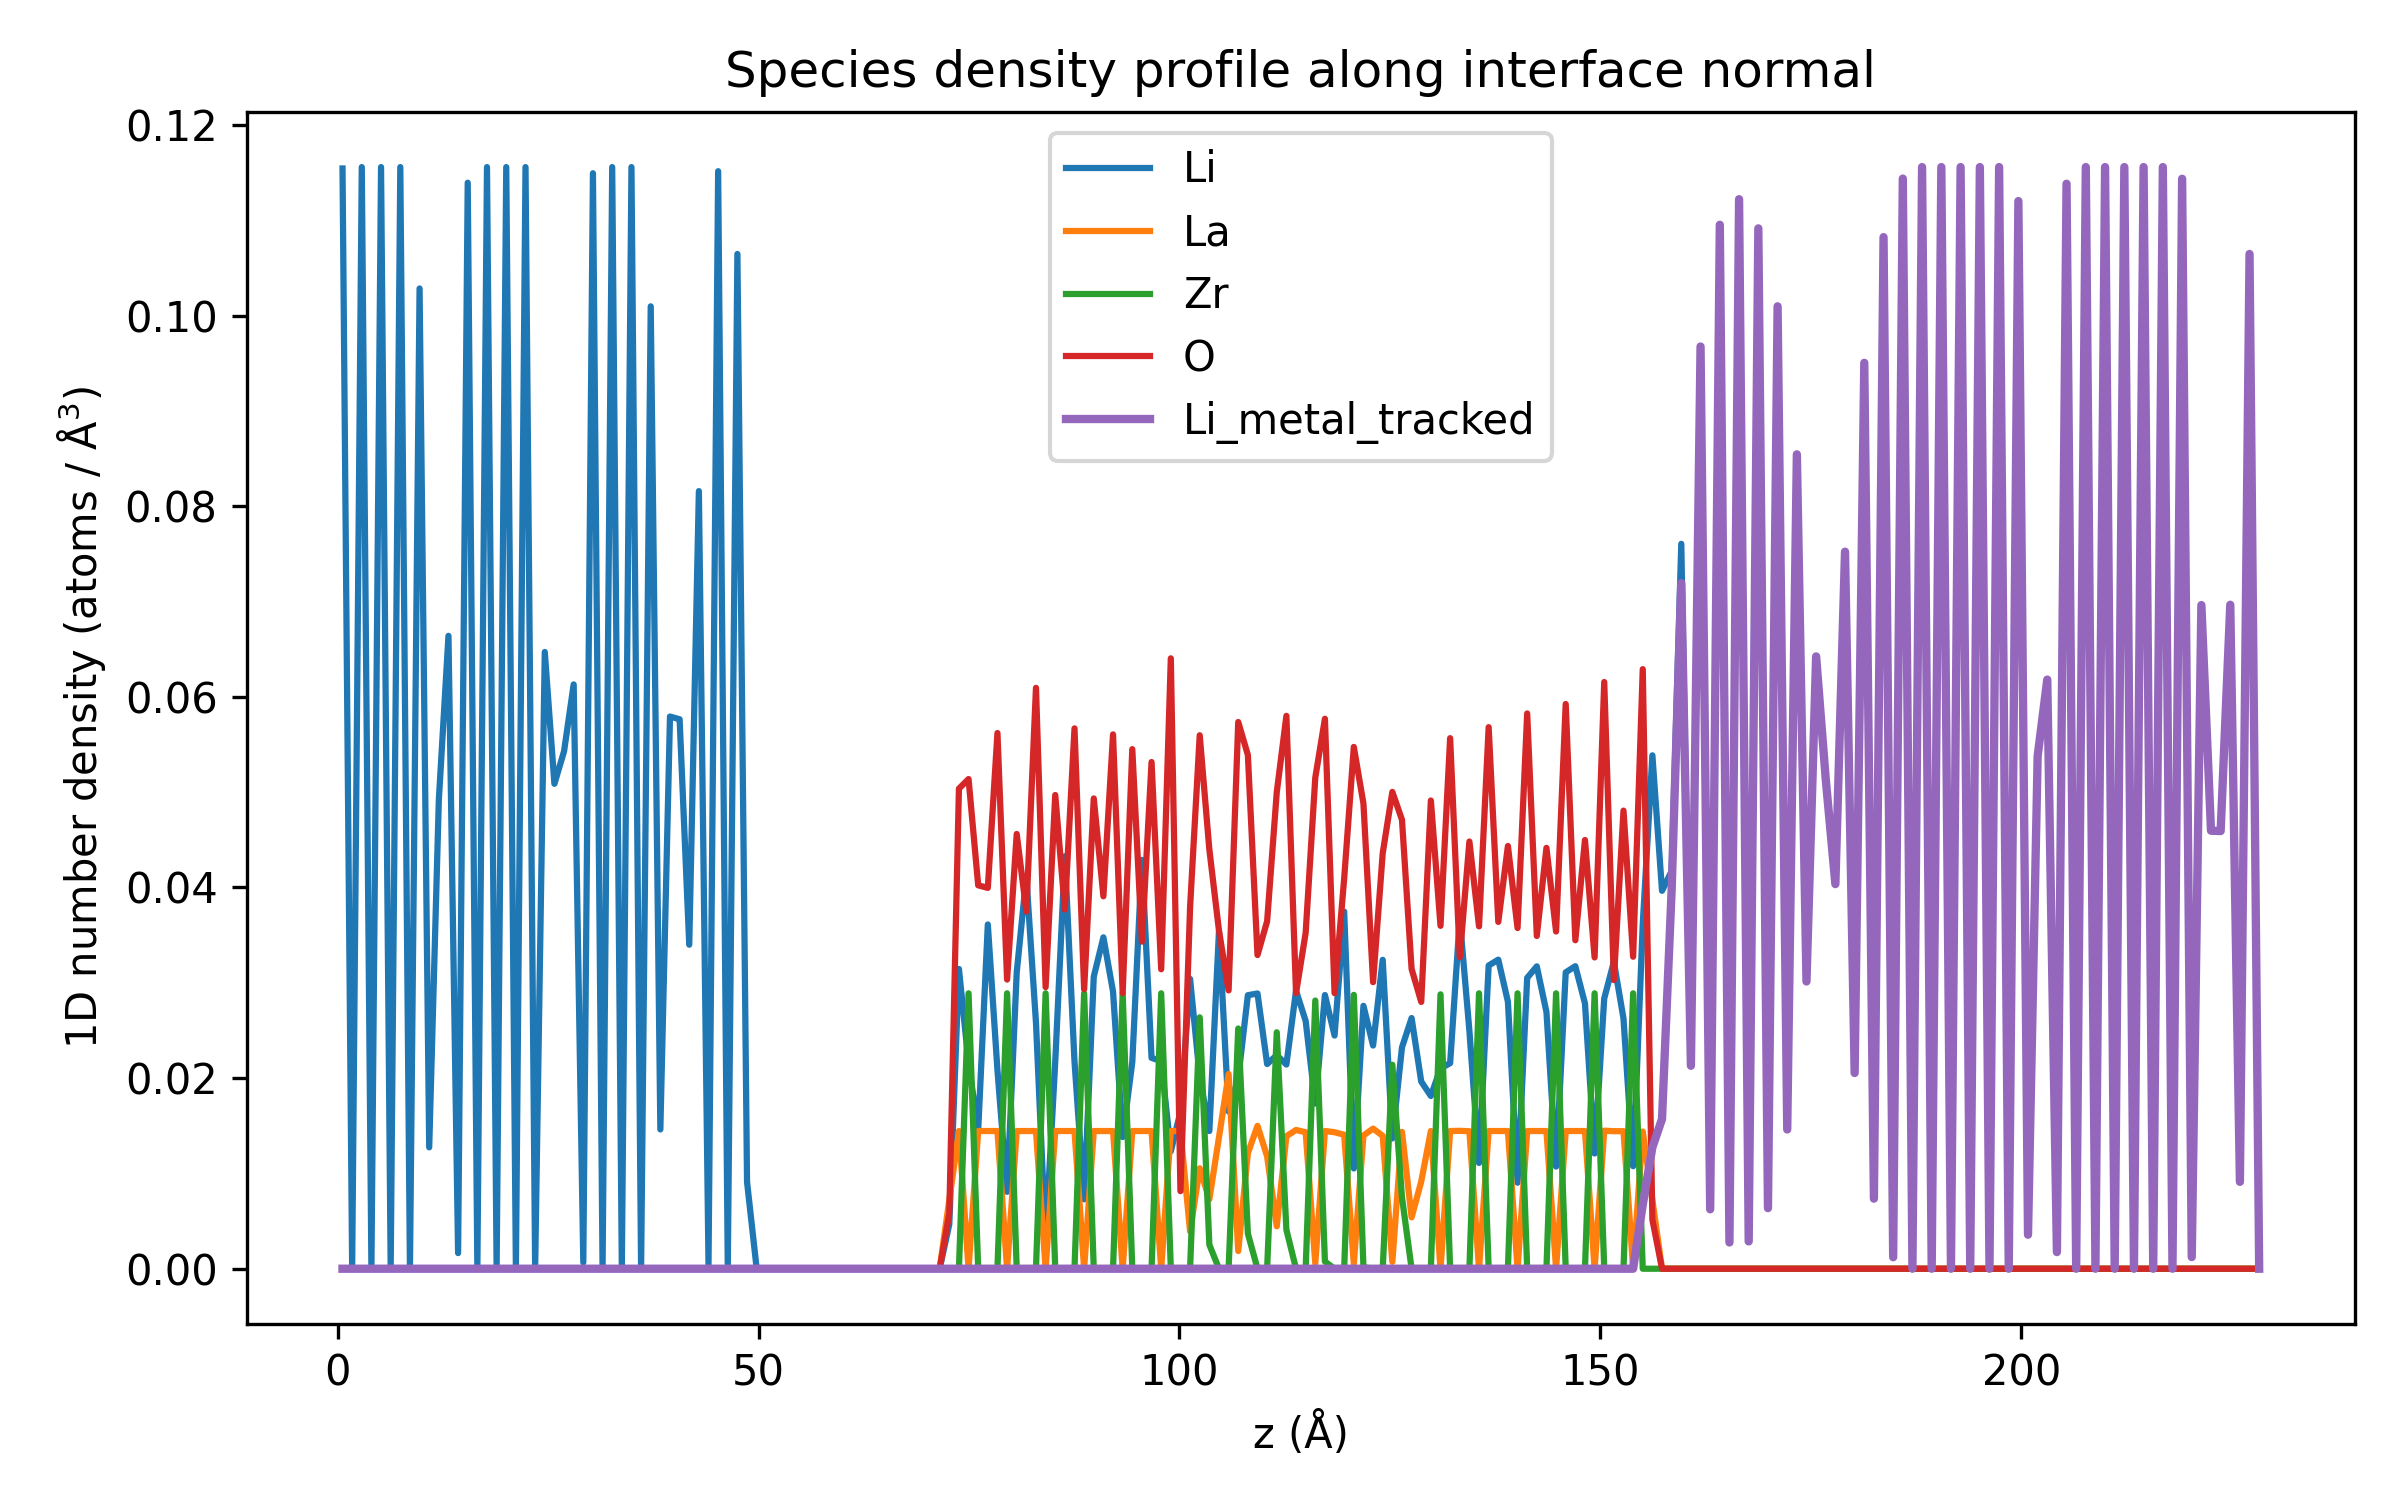
\includegraphics[width=0.7\textwidth]{z_density_profile.png}
\caption{
Species-resolved one-dimensional density profile along the interface normal for the Li/LLZO model. The LLZO host-lattice species (La, Zr, and O) remain confined to the oxide slab, while the tracked metallic Li atoms are primarily localized on the metal side. The interface remains spatially localized, with only limited shallow overlap in the interfacial region and no evidence of deep penetration of metallic Li into the LLZO slab over the simulated timescale.}
\end{figure}

The interface remains well-defined, with no evidence of mixing or structural collapse.

\paragraph{Mechanical stability --}

\begin{figure}[htbp]
\centering
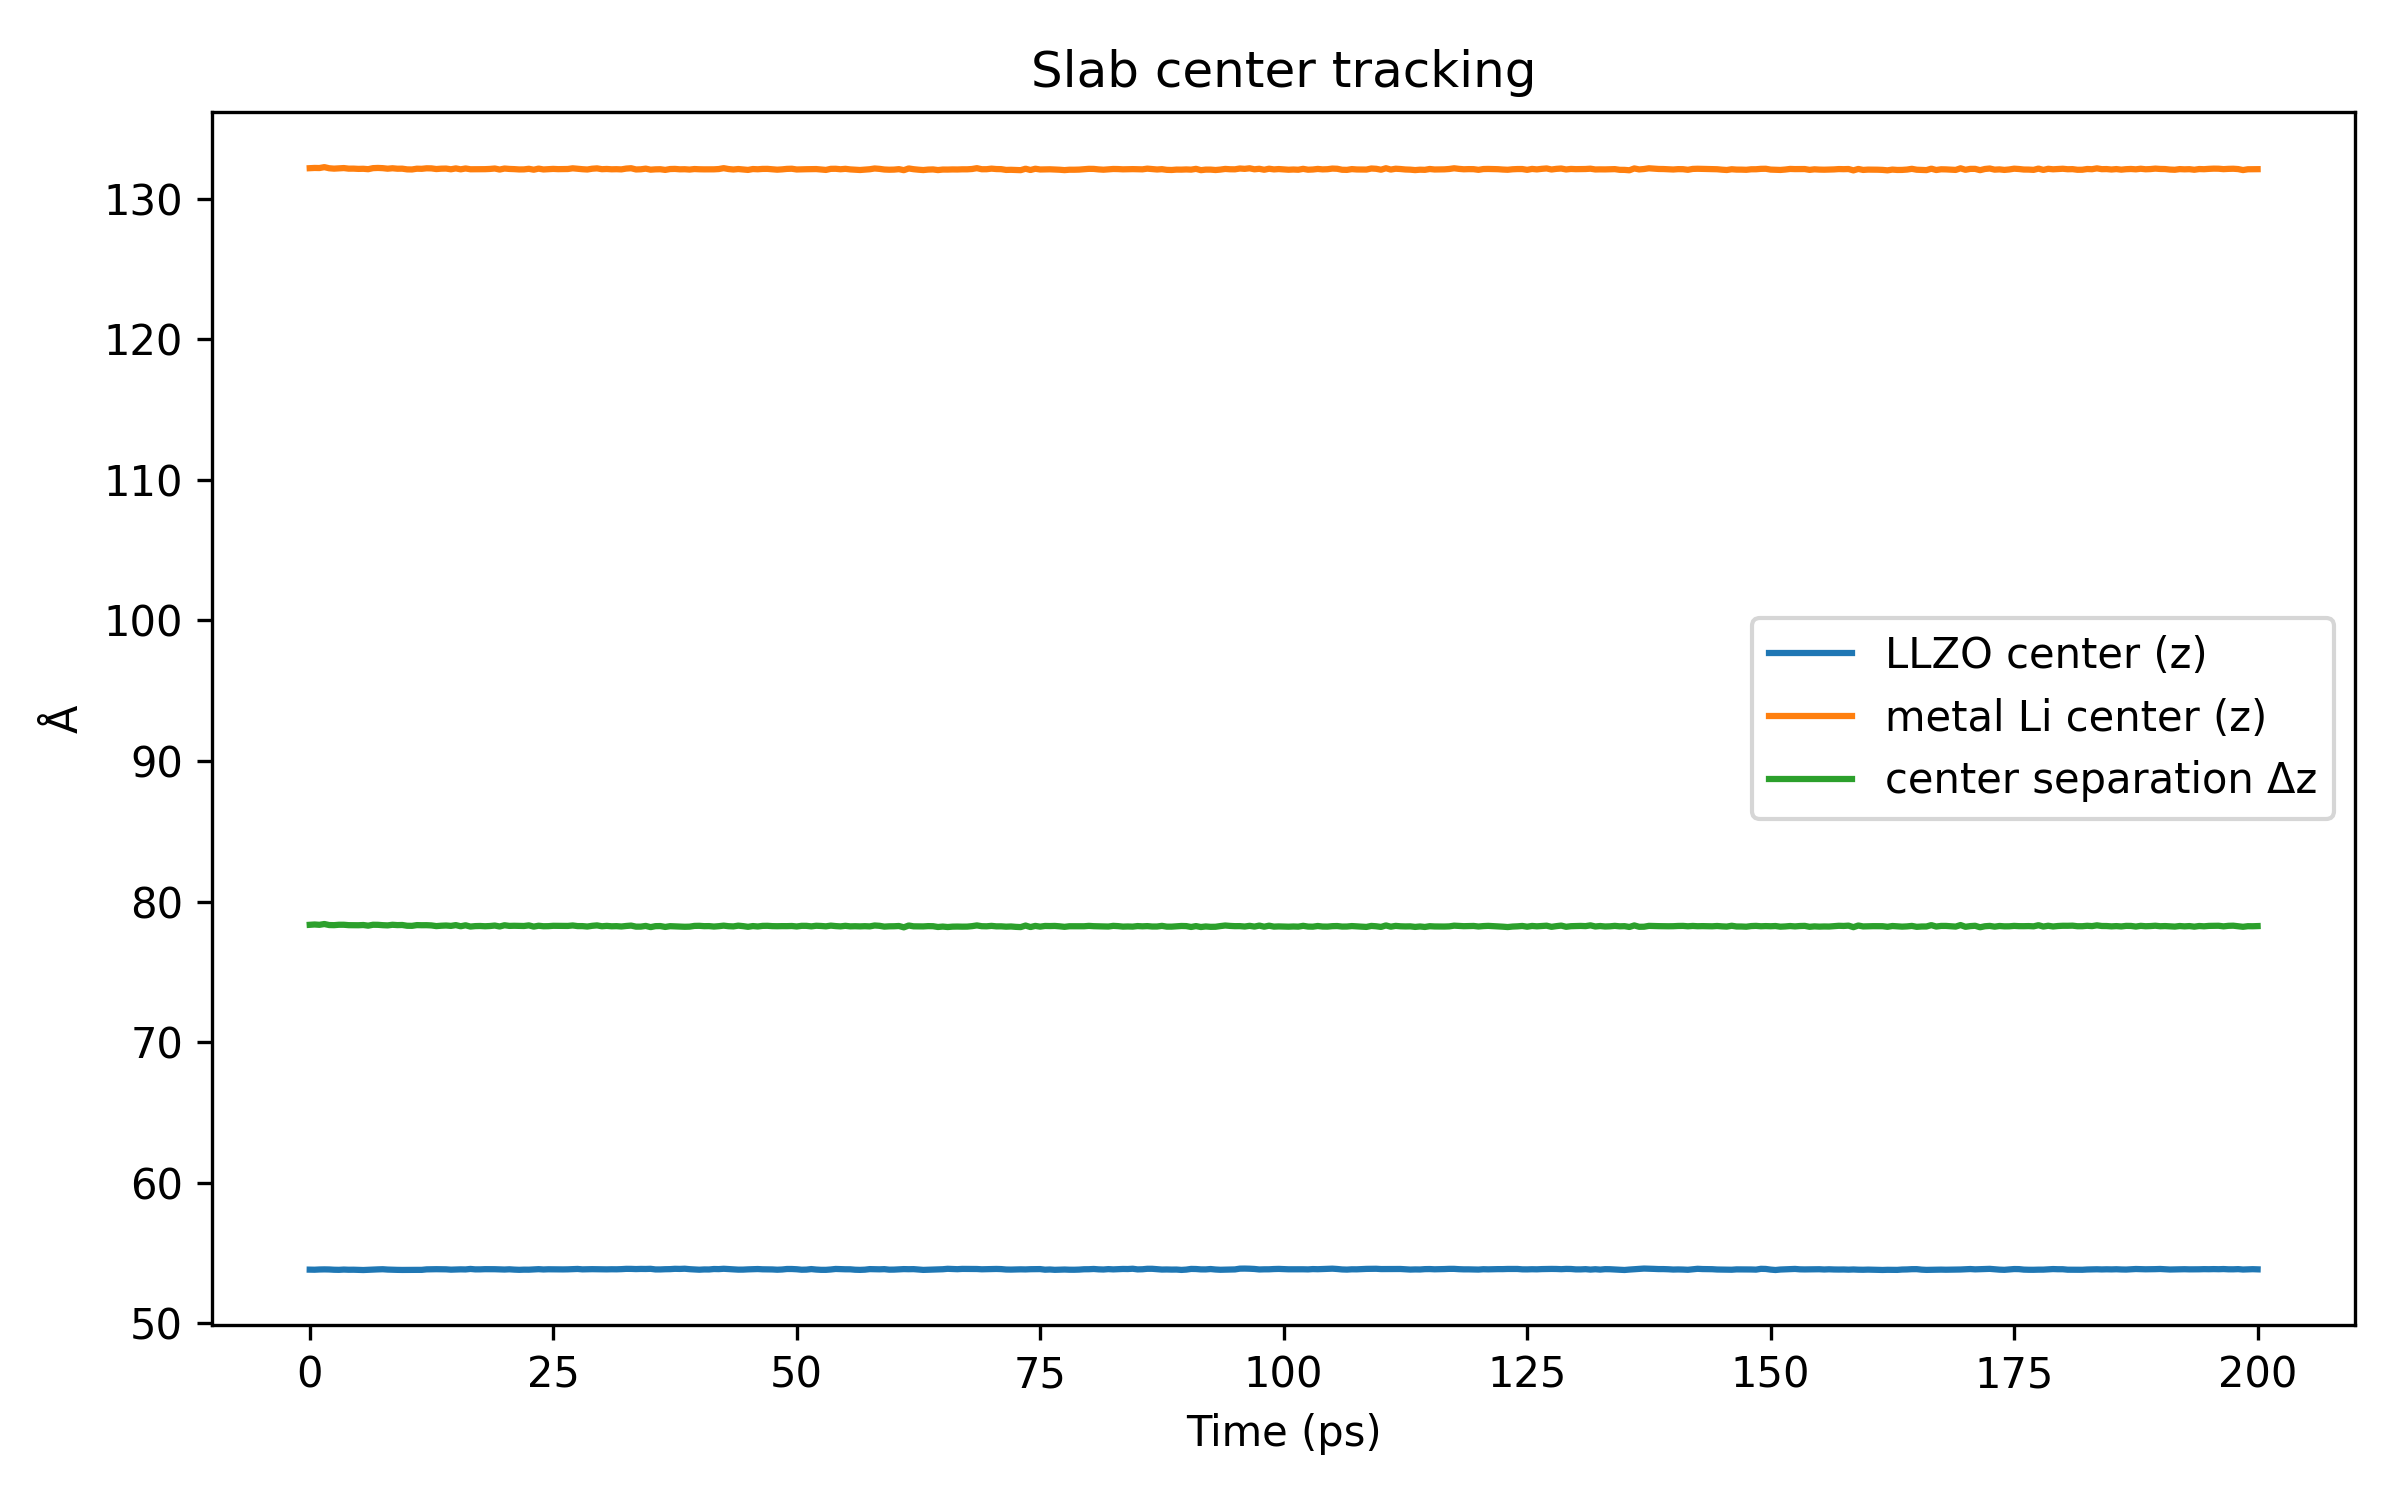
\includegraphics[width=0.7\textwidth]{slab_centers.png}
\caption{
Evolution of slab centers and their separation. The absence of drift confirms mechanical stability of the interface.
}
\end{figure}

No slab drift or artificial motion is observed.

\subsection{Physical Interpretation}

At 298 K, the Li(100)--LLZO(011) interface remains structurally stable over the 200 ps simulation timescale. Lithium atoms form a dynamic contact layer with surface oxygen atoms but do not penetrate into the LLZO lattice.

The LLZO framework remains intact, with no evidence of reconstruction, intermixing, or defect-driven instability. Observed fluctuations correspond to thermal motion rather than structural degradation.

\subsection{Outlook and Summary}

The qualitative MD results presented here motivate several directions for further
quantitative validation and methodological extension, which are discussed in the Outlook section of this chapter.

The Li(100)--LLZO(011) interface remains structurally stable over 200 ps at 298 K. No lithium insertion, intermixing, or framework degradation is observed. These results provide qualitative evidence for interfacial stability, while
highlighting the need for further quantitative analysis of transport properties ---
in particular NEB barrier calculations and pair distribution function comparisons
against DFT-labeled MD snapshots --- before strong conclusions about dynamics can be drawn.

\chapter{Challenges and Outlook}

\section*{Part I: Challenges Encountered}
\addcontentsline{toc}{section}{Part I: Challenges Encountered}

\section{Interface Construction at Scale}

Constructing physically meaningful Li--LLZO interface configurations required careful
coordination of slab geometries, lattice matching, and gap optimization. A key
practical difficulty was the combinatorial explosion of candidate interfaces: with
three Li orientations and six LLZO surface terminations, the lattice matching
procedure generated a large number of candidate supercell pairs, many of which
either exceeded the 10\% mismatch threshold or failed to converge during structural
relaxation. Of the 18 initial interface configurations constructed, only 13 survived
force convergence even with 2000 steps of relaxation, highlighting that automated interface construction pipelines must
include filtering steps. Extending this to more diverse LLZO surfaces and including
additional Li orientations would require further automation and more robust fallback
strategies for failed relaxations.

\section{Computational Cost of DFT Labeling}

The most significant bottleneck in the active learning loop was the cost of DFT
single-point calculations on large interface supercells. With system sizes ranging
from $\sim$450 to $\sim$1500 atoms and non-periodic boundary conditions along the
surface normal, each calculation required substantial GPU resources on the Frontier
supercomputer. Although the use of DFT-FE with high-order finite-element
discretization enabled efficient GPU-accelerated calculations, even a small labeling
batch of 20 structures at Iteration~0 required careful scheduling and queue management
across 64 compute nodes per job. This constraint directly motivated the Super-FPS
selection strategy: reducing the number of DFT calls per iteration was not merely a
matter of data efficiency, but a practical necessity imposed by computational resource
limits.

\section{Stability and Convergence of Finetuning in the Small-Data Regime}

Training accurate MLIPs from a dataset of 20--26 structures is inherently fragile.
The loss landscape is sensitive to the specific train--validation split, and early
experiments showed large variance in model quality across different random splits.
This necessitated the multi-split strategy (20 independent stratified splits per
iteration) and the selection of the best-performing model based on combined energy
and force validation metrics. Despite this mitigation, the force RMSE showed
greater sensitivity to data partitioning than the energy RMSE, consistent with
the higher-dimensional nature of force targets. Ensuring consistent generalization
required careful monitoring of both training and validation curves across all splits,
which added significant overhead to each active learning iteration.

\section{Out-of-Distribution Force Errors}

While the finetuned models demonstrated strong energy accuracy on OOD structures,
force predictions showed larger variance. In a small number of test cases (notably
Structure IDs 5 and 3 in Table~\ref{tab:ood_results}), the force RMSE of the finetuned
model exceeded that of the MACE-OMAT universal model. This behavior reflects a
fundamental tension in small-data finetuning: the model can learn to reproduce the
energy landscape of training structures while still exhibiting gradient inaccuracies
in sparsely sampled or geometrically atypical regions. Since molecular dynamics
simulations are driven entirely by forces, these localized force errors impose a ceiling
on the quantitative reliability of long-timescale dynamics. Addressing this limitation
would require either additional active learning iterations targeting high-error regions
or a rebalancing of the energy--force loss weighting.

\section{Limitations of MD-Based Sampling}

Molecular dynamics sampling with the pretrained or finetuned MACE model is inherently
constrained to configurations dynamically accessible from the starting geometry.
Interface stacking sequences that the model has never encountered --- such as the
tetragonal LLZO terminations from \citeauthor{Burov2024LiLLZOChargeTransfer}~\cite{Burov2024LiLLZOChargeTransfer} --- cannot
emerge from MD trajectories regardless of temperature or run length. This structural
limitation of MD-driven active learning was directly observed in Iteration~1, where two
external structures lay at latent-space distances approximately $1.5$--$2\times$ beyond
the maximum MD pool coverage radius. Their inclusion required explicit manual
construction and labeling, highlighting that purely MD-driven active learning is
insufficient for interfaces with combinatorially diverse surface chemistries.

\section{Absence of Long-Range Electrostatics}

A known limitation of the MACE framework, and of most short-ranged MLIPs, is the
absence of explicit treatment of long-range electrostatics. At the Li$|$LLZO interface,
charge transfer between lithium metal and the ceramic electrolyte is expected to
influence the interfacial potential and the driving force for lithium migration.
The present models capture local bonding environments faithfully but cannot explicitly
represent the space-charge layer or the associated electrostatic potential gradient.
This limits the applicability of the current models to structural and energetic
analyses and precludes direct simulation of electrochemical phenomena such as
interfacial charge transfer kinetics or the influence of applied bias on lithium
insertion.

\section{Scope of Molecular Dynamics Analysis}

The MD simulations presented in Chapter~4 are explicitly qualitative due to unreliable force errors on OOD structures. Only one
representative interface (Li(100)--LLZO(011)) was analyzed in detail over a 200~ps
trajectory at 298~K. While the results establish structural stability and the absence
of lithium penetration at this timescale, they do not provide quantitative transport
properties such as lithium diffusion coefficients, migration barriers, or
residence-time distributions. Extension to longer timescales and additional interface
configurations, as well as the use of NEB calculations for transition-state
characterization, remains as future work. A comparison of pair distribution functions between MLIP-MD trajectories and
DFT single-point labels on MD-sampled structures would provide the most direct
structural validation and is a priority for subsequent iterations.

\label{ch:future_work}

\section*{Part II: Outlook}
\addcontentsline{toc}{section}{Part II: Outlook}

\section{Additional Active Learning Iterations}

The active learning framework developed in this work was demonstrated through two
complete iterations, reducing energy errors from $\sim$600~meV/atom to below
5~meV/atom with only 26 DFT-labeled structures. The natural next step is to continue
this loop with additional interface configurations, particularly targeting the
high-error OOD structures identified in Table~\ref{tab:ood_results}. A third
iteration incorporating tetragonal LLZO terminations from
%% CHANGED: Iwasaki2021 → Iwasaki2022DFT_Li_LLZO_PSSB
\citeauthor{Burov2024LiLLZOChargeTransfer}~\cite{Burov2024LiLLZOChargeTransfer} and \citeauthor{Iwasaki2022DFT_Li_LLZO_PSSB}~\cite{Iwasaki2022DFT_Li_LLZO_PSSB} as explicit pool members, combined
with Super-FPS selection guided by the Iteration~1 model, is expected to further
reduce both energy and force errors in out-of-distribution regimes. Convergence of
the active learning loop can be assessed using the coverage radius $\rho(\mathcal{S},
\mathcal{P})$ as a stopping criterion: iteration terminates when the maximum
uncovered distance falls below a physically motivated threshold.

\section{NEB Calculations for Li Migration Barriers}
A critical outstanding validation is the comparison of lithium migration barriers
computed with the finetuned MACE models against DFT-NEB reference calculations.
Barrier heights are highly sensitive to force accuracy along the reaction coordinate,
making them a stringent test of MLIP reliability beyond aggregate RMSE metrics.
NEB barriers for representative Li migration pathways --- from the metal surface into
the LLZO lattice, and between adjacent sites within the near-interface region --- are
computed and compared against DFT reference values to directly assess whether the
finetuned models are suitable for studying ionic transport. Systematic discrepancies
will identify regions requiring targeted additional DFT labeling in subsequent
active learning iterations.
\section{Quantitative Transport Properties from Extended MD}

The present MD analysis was limited to 200~ps trajectories at 298~K for a single
interface. Extended simulations at higher temperatures (600--900~K) would enable
estimation of lithium diffusion coefficients across the interface. Mean-squared
displacement analysis stratified by atomic species and spatial region would quantify
the contribution of interface-mobile versus bulk-mobile lithium to the overall
transport. Such calculations are computationally tractable with the finetuned MACE
model, which evaluates forces at a fraction of the cost of DFT. A natural
structural validation --- comparing pair distribution functions $g(r)$ from
MLIP-MD trajectories against DFT single-point force labels on MD-sampled
structures, following the validation approach introduced in the final iteration
of the active learning loop --- would provide direct confirmation of structural
fidelity before drawing quantitative conclusions about transport.
\section{Extended Structural Validation via MD-Sampled DFT Labels}

The final iteration of the active learning loop introduces a held-out validation
strategy in which structures are sampled from MLIP-driven MD trajectories, labeled
with DFT single-point calculations, and used to assess model accuracy on
dynamically accessible configurations distinct from the FPS-selected training set.
This provides a more stringent and physically motivated test than static held-out
splits, since the MD structures reflect the actual distribution encountered during
interface simulations. Future work should extend this validation to a broader set
of interface configurations, terminations, and temperatures, building a
systematically curated benchmark of DFT-labeled MD snapshots against which
successive model iterations can be compared. Convergence of this benchmark error
across iterations would provide a principled stopping criterion for the active
learning loop that is grounded in dynamical accuracy rather than static coverage
statistics alone.
\section{Incorporation of Long-Range Electrostatics}

Extending the present models to include long-range electrostatic interactions would
substantially improve their physical realism at the Li$|$LLZO interface. Two
complementary approaches are available: (i) combining the short-ranged MACE model
with a long-range electrostatic correction via charge equilibration or a learned
charge model, and (ii) using recently proposed architectures such as MACE-E3 or
PaiNN-Q that include charge-state awareness within the message-passing framework.
The active learning pipeline developed here is directly compatible with either
extension, since the latent-space FPS and LoRA finetuning procedures are agnostic
to the specific MLIP architecture.

\section{Generalization to Other Solid Electrolyte Interfaces}

The methodology developed in this work --- pretrained universal MLIP, automated
interface construction, latent-space FPS, Super-FPS, progressive interface expansion,
and LoRA finetuning --- is fully general and not specific to the Li$|$LLZO system. Immediate candidate applications
include the Li$|$Li$_3$PS$_4$ (LPS) and Li$|$LIPON interfaces, both of which are
relevant to sulfide- and oxide-based all-solid-state batteries and present similarly
complex electro-chemo-mechanical environments. Extending the framework to Na-ion
solid electrolytes such as NaSICON-based interfaces would further broaden its
applicability. In each case, the primary cost is the DFT labeling of a small number
of FPS-selected structures; the infrastructure for MD sampling, embedding extraction,
and LoRA finetuning transfers directly.

\section{Mechanical Properties and Stress Evolution}

The present work focused on interfacial energetics and ion transport. An equally
important aspect of solid-solid battery interfaces is their mechanical integrity
under cycling-induced stress. The finetuned MACE models could be used to compute
the elastic response of Li--LLZO interface supercells and to simulate stress
evolution during lithium plating and stripping. Void formation, delamination, and
crack nucleation at the interface are known failure modes in all-solid-state batteries,
and atomistic simulations with accurate MLIPs could provide mechanistic insight into
these processes that is difficult to obtain experimentally.

\section{Improved Hyperparameter Optimization for \texorpdfstring{\\}{ } LoRA Finetuning}

The LoRA rank ($r = 5$) and scaling parameter ($\alpha = 1.0$) were selected by
hyperparameter tuning in this work, but a more systematic study of the rank--accuracy
tradeoff would be valuable. In particular, it is unclear whether the current rank
is sufficient to capture the chemical diversity of all relevant Li--LLZO interface
environments, or whether higher-rank adapters would improve force accuracy in
OOD regimes without incurring catastrophic forgetting. A natural extension, once a larger pool of DFT-labeled interface structures
is available from additional active learning iterations, is to perform a
systematic rank--accuracy study using the MD-sampled DFT labels described
above as the evaluation set, providing a physically grounded basis for
hyperparameter selection rather than relying on held-out static splits alone.


\chapter{Conclusions}

This thesis developed and evaluated a data-efficient active learning framework for
constructing machine learning interatomic potentials tailored to solid--solid
interfaces, with the Li$|$Li$_7$La$_3$Zr$_2$O$_{12}$ (LLZO) system as the primary
target. The central contribution is a systematic methodology that connects data
generation, latent-space-guided selection, parameter-efficient finetuning, and
physical validation into a coherent and generalizable pipeline. The following
conclusions are drawn from this work.

\paragraph{1. Latent-space diversity is the key driver of MLIP generalization at interfaces --}
Starting from a pretrained universal MACE-OMAT model, which exhibited energy errors
of $\sim$600~meV/atom and force errors of $\sim$136~meV/\AA\ on Li--LLZO interface
structures, systematic finetuning on FPS-selected configurations reduced these errors
to below 5~meV/atom and $\sim$50~meV/\AA\ on both training and validation sets. The
critical factor enabling this improvement with only 20 DFT-labeled structures in
Iteration~0 was the maximization of latent-space diversity through farthest point
sampling, which ensured that selected configurations spanned the boundaries of the
relevant chemical environment space rather than clustering near low-energy basins.

\paragraph{2. Super-FPS enables efficient structure selection from large MD pools --}
The two-stage Super-FPS algorithm introduced in Iteration~1 provides a computationally
tractable approach to selecting informative structures from pools of
$\sim$10$^3$--10$^5$ configurations. By combining a coarse diversity pass with a
fine complementarity pass seeded by the current training set, Super-FPS identifies
structures that are well separated from known configurations in latent space and
complement rather than duplicate existing training data. The six structures selected
by Super-FPS in Iteration~1 collectively served as the nearest neighbor for 922 of
$\sim$1320 pool structures (69.8\%), indicating broad coverage of the newly explored
configuration space.
\paragraph{3. LoRA finetuning enables targeted improvement without catastrophic forgetting --}
Parameter-efficient finetuning via low-rank adaptation with rank $r = 5$ and $\alpha
= 1.0$ allowed the model to be iteratively refined on small, task-specific datasets
while retaining the general chemical knowledge encoded in the pretrained MACE-OMAT
foundation model. The resulting adapted models showed consistent generalization across
multiple stratified train--validation splits, with training and validation errors in
close agreement, confirming the absence of significant overfitting despite the
small-data regime. The LoRA approach reduces the number of trainable parameters from
$\mathcal{O}(d^2)$ per layer to $\mathcal{O}(2rd)$, corresponding to less than 1\%
of the full model parameter count.

\paragraph{4. The finetuned models generalize to unseen and out-of-distribution interface structures --}
Evaluation on eight OOD test structures derived from Li$|$LLZO geometries
not present in the training data showed that both finetuned models substantially
outperformed the MACE-OMAT universal model. The Iteration~1 model achieved a
cohesive energy RMSE of 3.21~meV/atom compared to 15.51~meV/atom for the universal
model, and a force RMSE of 108.27~meV/\AA\ compared to 136.44~meV/\AA. The systematic
negative bias in the universal model's cohesive energy predictions --- consistent with
previously reported potential energy surface softening in universal MLIPs~\cite{Deng2025Softening} --- was
largely corrected by targeted finetuning, confirming that even a small number of
interface-specific DFT labels can substantially improve OOD reliability.

\paragraph{5. Interface energetics are physically consistent with prior DFT studies --}
Interface formation energies ($\gamma_{\mathrm{int}}$: 0.118--0.338~eV/\AA$^2$) and
work of adhesion ($W_{\mathrm{ad}}$: $-0.218$ to $-0.044$~eV/\AA$^2$) computed
with the finetuned model fall within the ranges reported in the prior first-principles
study of Iwasaki et al.~\cite{Iwasaki2022DFT_Li_LLZO_PSSB}, which covered 132 interface
models and reported $\gamma_{\mathrm{int}}$ values between 0.02 and 0.54~eV/\AA$^2$.
Consistent with that study's finding of no statistically significant difference between
orientations, the present results do not reveal a systematic preference for either
(001) or (111) interfaces. The dominant role of local atomic arrangement in
determining interface stability within a given crystallographic orientation was
confirmed, with (001) interfaces exhibiting substantially broader energy distributions
than (111) interfaces.

\paragraph{6. The Li(100)--LLZO(011) interface is structurally stable at 298~K over 200~ps --}
Molecular dynamics simulations of a representative interface confirmed the absence of
lithium penetration beyond 2~\AA\ into the LLZO lattice, preservation of the LLZO
framework with RMSD stabilizing at $\sim$0.28~\AA, and physically consistent atomic
mobility ordering ($\mathrm{Li}_{\mathrm{metal}} > \mathrm{Li}_{\mathrm{oxide}} >
\mathrm{framework}$). These results provide qualitative evidence for interfacial
stability, while highlighting the need for further quantitative validation ---
particularly NEB barrier calculations and pair distribution function comparisons
against DFT-labeled MD snapshots --- before drawing conclusions about ion
transport properties.

\paragraph{7. The methodology is general and broadly applicable --}
The active learning framework developed here --- pretrained foundation MLIP, automated
interface construction, latent-space FPS and Super-FPS, progressive interface
expansion, and LoRA finetuning --- does not depend on any feature specific to the
Li$|$LLZO system. The only requirements are a pretrained equivariant GNN model, a
DFT labeling oracle, and a sufficiently diverse set of interface configurations. The
framework is therefore directly transferable to other heterogeneous interfaces relevant
to energy materials, including sulfide electrolyte interfaces, sodium-ion systems, and
multi-component cathode--electrolyte contacts in next-generation solid-state batteries.

\bigskip
\noindent In summary, this work demonstrates that reliable MLIPs for complex
heterogeneous interfaces can be constructed from a small number of carefully selected
DFT calculations, provided that selection is guided by latent-space diversity rather
than random or energy-based heuristics. The combination of Super-FPS, LoRA
finetuning, and coverage-based validation provides a practical and principled
framework for extending the reach of foundation MLIPs into interfacial environments
where universal models currently fail. Further quantitative validation via NEB barrier calculations and pair distribution
function comparisons against DFT-labeled MD snapshots remains the primary direction
for establishing full physical reliability of the trained models.


\printbibliography
\newpage
\thispagestyle{empty}
\vspace*{\fill}
\begin{center}
\textit{Thank you.}
\end{center}
\vspace*{\fill}
\newpage
\thispagestyle{empty}
\vspace*{\fill}
\begin{center}
\textit{*********}
\end{center}
\vspace*{\fill}

\end{document}